\documentclass[11pt,a4paper,openany]{ctexbook}

\usepackage[margin=2.6cm]{geometry}
\usepackage{amsmath,amssymb,amsthm}
\usepackage{graphicx}
\usepackage{booktabs}
\usepackage{hyperref}
\usepackage{xcolor}
\usepackage{listings}
\usepackage{caption}

\graphicspath{{chapters/ch01_introduction/figures/}{chapters/ch02_trends_in_a_time_series/figures/}{chapters/ch03_stationary_time_series/figures/}{chapters/ch04_linear_time_series/figures/}{chapters/ch05_a_review_of_some_results_from_multivariate_a/figures/}{chapters/ch06_the_autocovariance_and_partial_covariance_of/figures/}{chapters/ch07_prediction/figures/}{chapters/ch08_estimation_of_the_mean_and_covariance/figures/}{chapters/ch09_parameter_estimation/figures/}{chapters/ch10_spectral_representations/figures/}{chapters/ch11_spectral_analysis/figures/}{chapters/ch12_multivariate_time_series/figures/}{chapters/ch13_nonlinear_time_series_models/figures/}{chapters/ch14_consistency_and_asymptotic_normality_of_esti/figures/}{chapters/ch15_residual_bootstrap_for_estimation_in_autoreg/figures/}{chapters/appA_background/figures/}{chapters/appB_mixingales_and_physical_dependence/figures/}}
\hypersetup{colorlinks=true, linkcolor=blue!50!black, urlcolor=blue!60!black}
\lstset{
  basicstyle=\ttfamily\small,
  breaklines=true,
  frame=single,
  columns=fullflexible,
  backgroundcolor=\color{gray!7}
}

\newtheorem{definition}{定义}[section]
\newtheorem{theorem}{定理}[section]
\newtheorem{lemma}{引理}[section]
\newtheorem{proposition}{命题}[section]
\newtheorem{example}{例}[section]

\title{A Course in Time Series Analysis\\中文讲义与 Python 实践}
\author{基于原书内容整理的中文主导教学讲义}
\date{\today}

\begin{document}
\maketitle
\frontmatter
\tableofcontents
\mainmatter

% Source: chapters/ch01_introduction/第01章_Introduction_导论.tex
\chapter{Introduction / 导论}
\section*{本章学习目标}

本章的作用是建立时间序列分析的入口视角。原文从最简单的独立随机变量出发，说明时间序列与经典统计的核心差别：观测值按照时间排序，并且相邻或相隔若干期的观测之间常常存在依赖结构。正是这种依赖结构，使预测、滤波、趋势识别和周期识别成为可能。

完成本章后，应能够：
\begin{itemize}
  \item 说明什么是等间隔观测的时间序列；
  \item 区分无相关随机序列和具有时间结构的真实序列；
  \item 理解 SOI、Nasdaq、太阳黑子、气温等数据在时间序列课程中的典型用途；
  \item 将原文中的 R 入门绘图思路改写为 Python 实践；
  \item 理解线性滤波的基本表达式以及它在后续章节中的作用。
\end{itemize}

\section{时间序列的基本概念}

时间序列是一组按时间顺序记录的观测值，记作
\[
  x_t,\quad t \in \mathbb{Z}.
\]
观测方式可以有多种：在一个连续区间上观测、在区间中随机抽样观测，或者在固定的等间隔时间点观测。本课程主要讨论第三种情形，即观测点之间间隔相同。为了便于数学表达，通常将时间下标写成整数集合
\[
  \mathbb{Z}=\{\ldots,-1,0,1,2,\ldots\}.
\]

最简单的时间序列是独立同分布随机变量序列。如果每个观测之间相互独立且均值为 0，那么从图形上通常看不到稳定的趋势、周期或可利用的依赖结构。此时，对下一期观测的最佳朴素预测往往只是均值 0。

\begin{figure}[htbp]
  \centering
  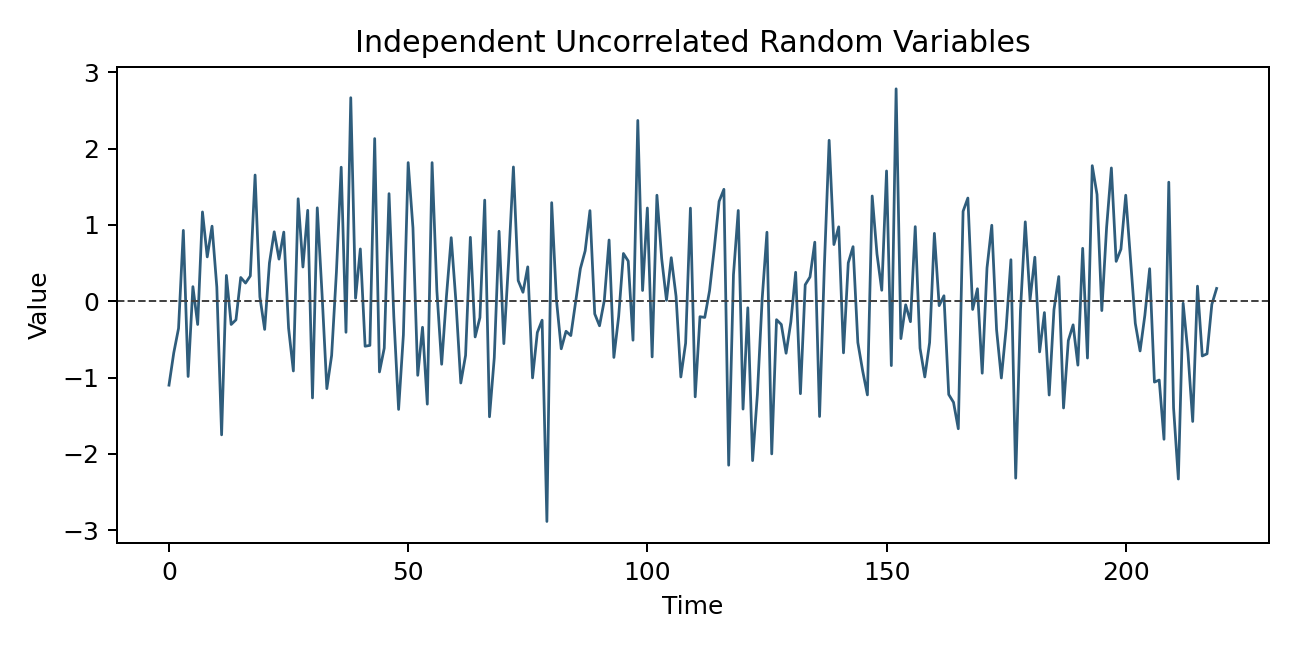
\includegraphics[width=0.86\textwidth]{ch01_fig01_white_noise.png}
  \caption{独立无相关随机变量序列。该图对应原文 Figure 1.1 的教学意图：序列围绕 0 上下波动，但没有明显趋势或周期。}
\end{figure}

时间序列分析真正关心的是观测之间的依赖。若当前值与过去值相关，过去信息就可能帮助我们预测未来；若序列中存在周期结构，我们可以识别周期；若均值随时间缓慢变化，我们需要估计趋势。

\subsection{原文逐段补充}

原文首先强调，时间序列并不只是“一串数”，而是一串在一段时间中观测到的数值。观测可以覆盖整个时间区间，也可以是在某个区间内随机抽样获得，还可以是在固定时间点上获得。不同的时间抽样方式会导致不同的数据分析方法。本课程选择最常见也最便于建立理论的设定：观测发生在固定且等间隔的时间点上。因此，后续都把观测写为
\[
  \{x_t:t\in\mathbb Z\},
\]
其中
\[
  \mathbb Z=\{\ldots,0,1,2,\ldots\}.
\]
这一定义看似简单，但它决定了后续所有滞后、差分、滤波、预测和频域分析的基本语言。

原文随后从最简单的时间序列例子开始：独立且不相关的随机变量。它们当然也按时间排列，因此形式上是时间序列；但从图形上看，这类序列没有清楚的模式。原文 Figure 1.1 展示的白噪声序列围绕 0 上下波动，既看不到趋势，也看不到周期。若要求预测下一期观测，最自然的预测值就是 0，也就是图中看起来像均值的位置。

这一点用来说明时间序列与经典统计的关键差别。经典统计常从独立样本出发，而时间序列最有价值的地方恰恰在于观测之间可能存在依赖。依赖意味着过去信息可能帮助预测未来，也意味着不能简单套用独立样本的标准误、置信区间和显著性检验。原文要求读者记住 Figure 1.1 的白噪声图，并把它与随后四个真实数据例子比较：真实时间序列通常会显示出某些模式。

\section{典型时间序列数据}

原文用四类数据说明时间序列问题的多样性。

\subsection{南方涛动指数}

南方涛动指数（Southern Oscillation Index, SOI）描述塔希提和达尔文之间海平面气压差的波动，是衡量厄尔尼诺现象强度的重要指标之一。原文使用 1876 年 1 月到 2014 年 7 月的月度 SOI 数据，并强调一个主要目标：寻找数据中的模式，特别是周期性。

在没有直接附带原始 SOI 数据文件的情况下，本章 Python 脚本生成一个具有周期成分和持续性噪声的模拟 SOI 序列，用于复现“月度气候指标具有波动结构”的教学场景。

原文指出，SOI 是衡量厄尔尼诺效应强度的指标。它记录塔希提与达尔文之间地表气压差的波动。Figure 1.2 给出 1876 年 1 月到 2014 年 7 月的月度 SOI 图形，并特别提醒：1930 年以前的数据可靠性存在一定疑问。原数据来自澳大利亚气象局网页。对于这类气候指数，本课程关注的主要问题不是单个观测值的大小，而是序列中是否存在可重复的模式，尤其是周期性。

\begin{figure}[htbp]
  \centering
  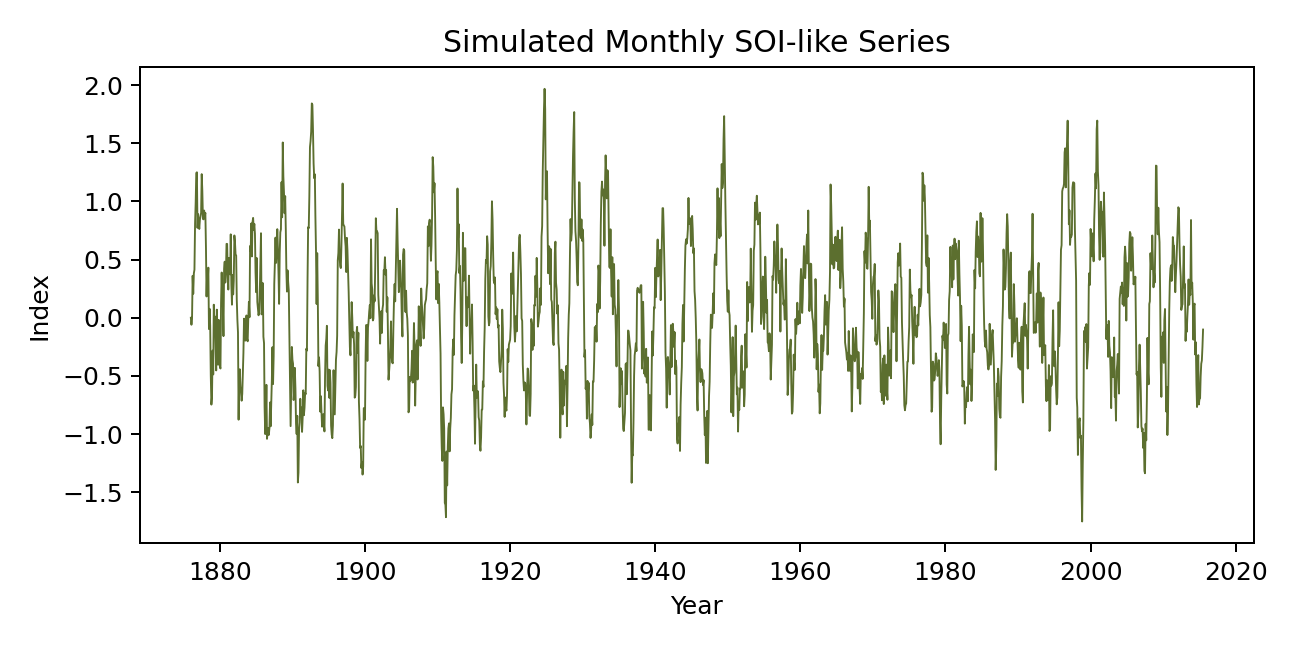
\includegraphics[width=0.86\textwidth]{ch01_fig02_simulated_soi.png}
  \caption{模拟的月度 SOI 型序列。图中可见慢周期波动和持续性噪声，这类结构适合引出周期检测和相关噪声问题。}
\end{figure}

\subsection{Nasdaq 金融数据}

原文展示了 1985 年 10 月 1 日至 2014 年 8 月 8 日的 Nasdaq 日收盘价。金融时间序列的直接动机常常是预测收益、风险或波动率。对于价格序列本身，常见现象包括长期增长、非平稳性和波动聚集；后续章节会逐步讨论差分、ARMA、ARCH/GARCH 等工具。

原文 Figure 1.3 使用的是 Nasdaq 日收盘价，时间范围为 1985 年 10 月 1 日到 2014 年 8 月 8 日。数据来源包括 Yahoo Finance 的历史数据，也提到美国联邦储备相关数据页面。原文用半开玩笑的方式说，对于这类金融数据，目标当然是“赚钱”；从统计角度说，核心任务是预测未来，特别是预测未来波动率。金融价格序列常表现为非平稳水平、长期变化和阶段性剧烈波动，因此后续需要研究收益率、差分、条件方差和非线性模型。

\subsection{太阳黑子数据}

太阳黑子数量是经典时间序列案例。太阳活动具有明显的周期性，因此适合用来引出周期识别、谱分析和长期预测。下面的 Python 图使用 \texttt{statsmodels} 内置太阳黑子数据。

太阳黑子活动由太阳表面可见黑子数量衡量。原文说明，近些年太阳黑子重新受到关注，是因为高太阳活动时期可能严重干扰通信网络。Figure 1.4 给出 1700 年到 2013 年年度太阳黑子数，数据来自 SILSO 数据页面。此类数据的目标有两个：一是寻找序列中的模式，二是预测未来太阳黑子活动。由于太阳黑子序列具有明显的周期波动，它是本课程引入周期检测和谱分析的经典案例。

\begin{figure}[htbp]
  \centering
  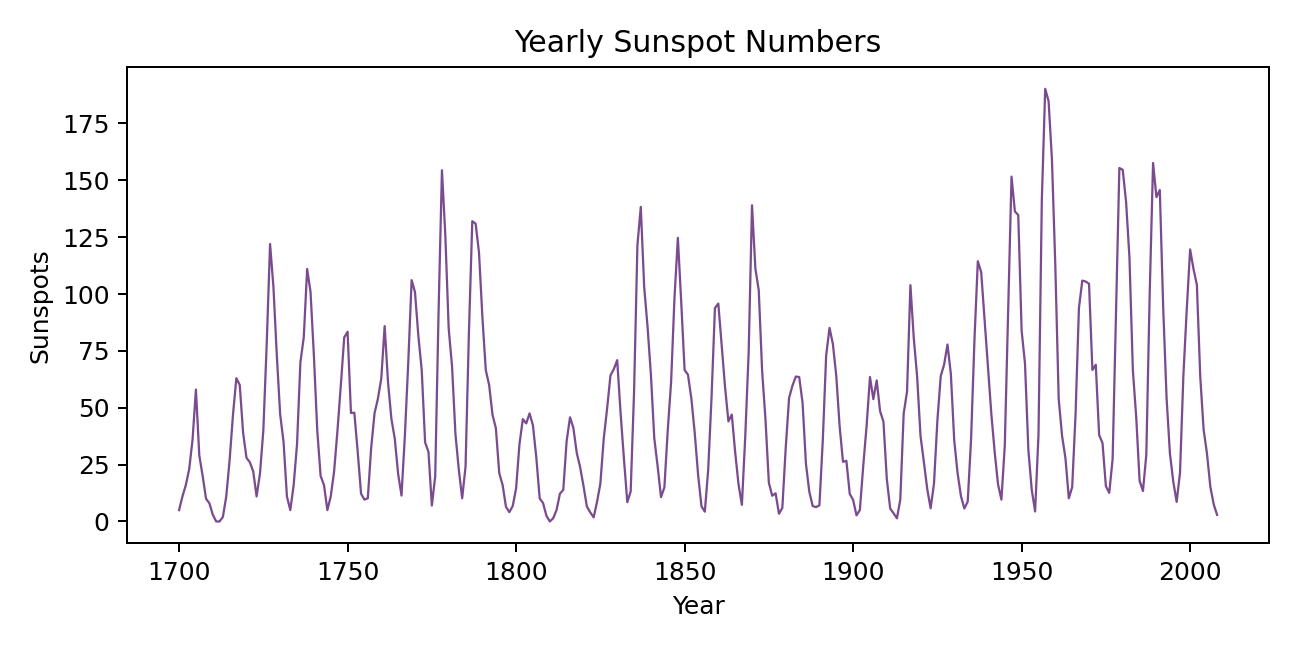
\includegraphics[width=0.86\textwidth]{ch01_fig03_sunspots.png}
  \caption{年度太阳黑子数量。可观察到明显的周期波动，是后续研究周期和谱密度的典型案例。}
\end{figure}

\subsection{年度与月度气温数据}

气温异常序列常用于研究长期均值变化。原文指出，若目标是检测全球变暖，就不能只画一条趋势线后直接下结论，还需要时间序列统计推断来判断趋势估计是否显著。原因在于，时间序列观测通常不是独立样本，相关性会改变估计量的标准误和显著性判断。

原文考虑两类全球温度数据：1880 年到 2013 年的年度温度异常，以及 1996 年 1 月到 2014 年 7 月的月度平均温度。Figure 1.5 展示年度温度异常，Figure 1.6 展示月度温度。数据来源为 NASA GISS 提供的全球温度数据文件。研究这类数据时，一个自然问题是检测全球变暖，即检测平均温度是否存在长期变化或上升。通常做法是对数据拟合趋势函数，但原文强调，仅仅拟合趋势线并不足够；必须使用更细致的时间序列分析，判断趋势估计是否具有统计显著性。原因在于温度序列存在相关性和季节结构，不能把每个观测简单当作独立样本。

\section{从 R 代码到 Python 实践}

原文提醒读者熟悉 R，并给出了 \texttt{ts()} 和 \texttt{plot.ts()} 的基本用法。在 Python 中，类似工作通常由 \texttt{pandas} 的时间索引、\texttt{matplotlib} 绘图和 \texttt{statsmodels} 建模共同完成。

\begin{lstlisting}[language=Python, caption={Python 中构造月度时间序列的基本模式}]
import pandas as pd

dates = pd.date_range("1876-01-01", periods=120, freq="MS")
series = pd.Series(range(120), index=dates)
series.plot()
\end{lstlisting}

原文第 1.2 节说明，课程中的很多方法和概念会用 R 语言展示，因此不熟悉 R 的读者应先掌握基础语法。原文给出了读取数据和构造时间序列对象的示例：假设 SOI 数据保存在主目录中，可以用 \texttt{scan()} 读入；随后用 \texttt{ts()} 创建时间序列对象。例如，月度数据从 1876 年 1 月开始，频率设置为 12，因为一年有 12 个观测。用 \texttt{plot.ts()} 可以直接画出时间序列图。

R 代码中的 \texttt{start=c(1876,1)} 表示起始年份为 1876 年、起始月份为 1 月；\texttt{frequency=12} 表示每年 12 个观测。原文还特别指出，正确地给图形标注日期非常有用。R 中可以借助 \texttt{zoo} 包和 \texttt{as.Date()} 函数处理日期。在 Python 中，与之对应的做法是使用 \texttt{pandas.date\_range()} 创建时间索引，用 \texttt{Series} 或 \texttt{DataFrame} 保存观测，再用 \texttt{matplotlib} 或 \texttt{pandas} 内置绘图函数作图。

原文 R 代码逐行含义如下。第一行
\[
  \texttt{soi <- scan("\textasciitilde/soi.txt")}
\]
表示从文本文件读入 SOI 数据。第二行用 \texttt{ts()} 把数值向量转换为带时间属性的对象，其中起点是 1876 年 1 月，频率是 12。原文代码片段中变量名写成 \texttt{monthlytemp}，结合上下文应理解为要传入已经读入的月度序列。随后 \texttt{plot.ts(soi1)} 直接绘图。若要在 Python 中保持同样信息，关键是不要只保存裸数组，而要同时保存日期索引；否则图形横轴无法正确显示年份和月份。

本章原文的六幅图也各有用途。Figure 1.1 是独立不相关随机变量，用作“没有模式”的基准图。Figure 1.2 是月度 SOI，用于展示气候指标中的周期和低频波动。Figure 1.3 是 Nasdaq 日收盘价，用于提示金融价格序列的非平稳性和预测动机。Figure 1.4 是太阳黑子年度数据，用于展示明显周期。Figure 1.5 是年度全球温度异常，用于引出长期趋势检测。Figure 1.6 是月度温度序列，用于说明高频季节变化和长期变化可能同时出现。把这些图放在同一章，是为了让读者从一开始就看到时间序列问题的多样性。

本章的完整实践脚本位于：
\[
  \texttt{scripts/ch01\_generate\_figures.py}.
\]
运行后会在 \texttt{figures/} 目录生成本章所有图像。

\section{时间序列滤波}

为了突出某些特征或去除不需要的特征，我们经常对原始时间序列做变换。原文特别强调线性变换。设原始序列为 \(\{X_t\}\)，变换后的序列为 \(\{Y_t\}\)，则线性滤波可以写作
\[
  Y_t = \sum_{j=-\infty}^{\infty} h_j X_{t-j},
\]
其中 \(\{h_j\}\) 是一组权重。

本课程后续主要使用两类线性变换：
\begin{itemize}
  \item 用于估计随时间变化的均值函数，例如移动平均平滑；
  \item 用于理解观测序列中的随机部分，例如频域变换和滤波。
\end{itemize}

原文第 1.3 节把这种操作称为 filtering time series。很多时候，我们会变换数据以突出想看的特征，或移除不想要的特征。常见变换包括对数变换和线性变换。对时间序列来说也是如此：变换后的序列可能比原序列更容易分析，或者显示出原图中不明显的特征。本讲义主要关注线性变换，因为它们既容易分析，又能直接连接到移动平均、差分、滤波和 Fourier 方法。

在线性滤波公式
\[
  Y_t=\sum_{j=-\infty}^{\infty}h_jX_{t-j}
\]
中，权重 \(h_j\) 决定滤波器的作用。若权重集中在当前和附近时间点并且总和为 1，滤波器通常起到平滑作用；若权重之和为 0，例如一阶差分 \(Y_t=X_t-X_{t-1}\)，滤波器则会削弱低频趋势。原文在本章末尾预告，下一章将研究时间变化均值的估计，并会使用这里提到的变换。

\begin{figure}[htbp]
  \centering
  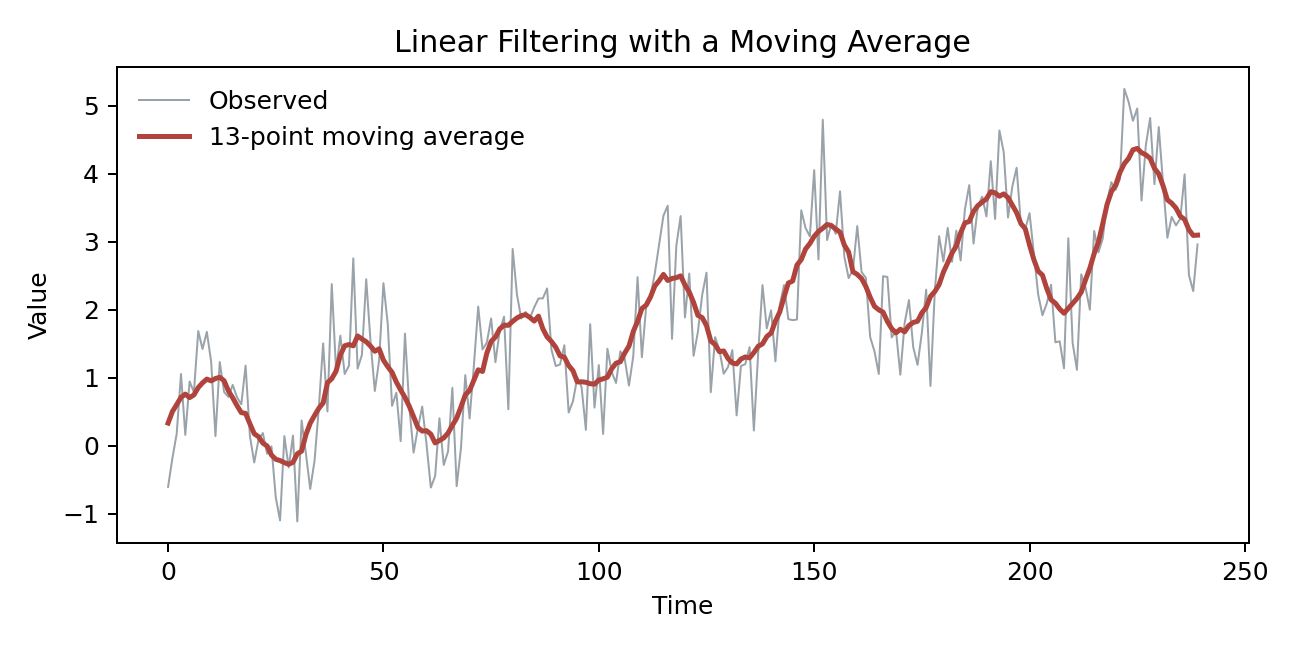
\includegraphics[width=0.86\textwidth]{ch01_fig04_filtering.png}
  \caption{移动平均滤波示例。灰色曲线是带噪声观测，红色曲线是 13 点移动平均，展示了线性滤波如何突出低频趋势。}
\end{figure}

\section{术语}

\begin{description}
  \item[iid] independent and identically distributed，独立同分布。它是最简单的时间序列模型，但通常不是实际时间序列分析的终点。
  \item[预测] 利用过去和当前信息推断未来观测。
  \item[趋势] 序列均值随时间发生的系统性变化。
  \item[周期] 序列中以某种频率重复出现的结构。
  \item[滤波] 通过加权组合过去、当前或未来观测来变换序列。
\end{description}

原文第 1.4 节只列出了一个术语：iid，即 independent, identically distributed，独立同分布随机变量。原文称它是“你可能处理的最简单时间序列”。这句话的意思是：iid 序列虽然也按时间排列，但时间下标没有带来额外信息；任意一期与其他期独立，且分布相同。因此，它是时间序列理论的基准模型。后续所有复杂模型都可以与 iid 白噪声比较：如果残差已经接近 iid，说明模型较好地解释了序列中的可预测结构；如果残差仍有趋势、周期或相关性，说明模型还不充分。

因此，第 1 章完整内容可以概括为一条主线：先定义等间隔时间序列，再用白噪声说明“无结构”情形，然后用四类真实数据说明趋势、周期、波动和预测问题，接着给出 R 中创建和绘制时间序列对象的基本方法，最后引入线性滤波作为后续章节的共同工具。这里没有复杂定理，但每个概念都会在后面反复出现：第 2 章处理趋势，第 3 章处理平稳性，第 4 章处理线性模型，第 7 章处理预测，第 10 和第 11 章处理频域结构，第 13 章处理金融波动。

\section{Python 工程实践}

在本章目录下运行：
\begin{lstlisting}[language=bash]
python scripts/ch01_generate_figures.py
\end{lstlisting}

脚本生成四张图：
\begin{itemize}
  \item \texttt{ch01\_fig01\_white\_noise.png}：独立无相关随机序列；
  \item \texttt{ch01\_fig02\_simulated\_soi.png}：模拟 SOI 型月度序列；
  \item \texttt{ch01\_fig03\_sunspots.png}：太阳黑子年度序列；
  \item \texttt{ch01\_fig04\_filtering.png}：移动平均滤波。
\end{itemize}

\section{练习提要}

原文第 1 章的练习性质主要体现在读图、数据导入和基本滤波操作中。学习时可围绕下列方向展开：
\begin{itemize}
  \item 用 Python 构造等间隔时间索引，并绘制白噪声、周期序列和带趋势序列；
  \item 比较 SOI、Nasdaq、太阳黑子和温度数据中趋势、周期和相关性的差异；
  \item 对同一序列尝试不同移动平均窗口，观察滤波后低频趋势和高频波动如何变化；
  \item 把原文中的 \texttt{ts()}、\texttt{plot.ts()} 思路改写为 \texttt{pandas.Series} 和 \texttt{matplotlib} 工作流。
\end{itemize}

\section*{本章小结}

第 1 章的重点不是推导复杂模型，而是建立问题意识：时间序列数据的顺序和依赖结构很重要。独立随机变量序列几乎没有可预测结构，而气候、金融、太阳活动和温度序列往往具有趋势、周期、波动聚集或相关噪声。后续章节会围绕这些结构展开：先研究趋势，再研究平稳性、线性模型、预测、估计、谱分析和非线性模型。

\clearpage
% Source: chapters/ch02_trends_in_a_time_series/第02章_Trends_in_a_time_series_时间序列中的趋势.tex
\chapter{Trends in a time series / 时间序列中的趋势}
\section*{本章学习目标}

本章研究时间序列中的均值函数或趋势项。原文把一个典型时间序列写成
\[
  Y_t=\mu_t+\varepsilon_t,
\]
其中 \(\mu_t=E(Y_t)\) 是不能由随机误差解释的系统性部分，\(\varepsilon_t\) 是残差或误差项。时间序列分析中常见的两类任务是：估计 \(\mu_t\)，或者对 \(\{Y_t\}\) 做变换，使趋势项在变换后尽量消失，从而集中研究残差的依赖结构。

完成本章后，应能够：
\begin{itemize}
  \item 使用参数模型描述线性、多项式、非线性和季节趋势；
  \item 用最小二乘和非线性最小二乘估计趋势参数；
  \item 理解差分如何移除确定性趋势和随机趋势，以及过度差分的风险；
  \item 说明滚动窗口、筛估计等非参数趋势估计思想；
  \item 掌握离散傅里叶变换、周期图和周期检测的基本公式；
  \item 将原文中的 R 实践改写为 Python 图形与计算流程。
\end{itemize}

\section{参数趋势}

在许多时间序列问题中，除了观测值 \(Y_t\) 外，还可以使用解释变量。解释变量可以是外生变量，也可以是时间 \(t\) 本身或时间的函数，因为时间下标具有明确顺序。所谓参数模型，是指除有限个未知参数外，其余结构都已知的模型。

最简单的参数趋势是线性模型。原文给出的两个常用形式为
\begin{align}
  Y_t &= \beta_0+\beta_1 t+\varepsilon_t, \tag{2.1}\\
  Y_t &= \beta_0+\beta_1 t+\beta_2 t^2+\varepsilon_t. \tag{2.2}
\end{align}
这些模型称为线性模型，是因为它们对未知参数 \(\beta_0,\beta_1,\beta_2\) 是线性的，而不是因为趋势曲线一定是直线。

参数也可以出现在非线性函数内部。例如平滑转移模型可写为
\begin{equation}
  Y_t=\frac{1}{1+\exp\{\beta_0(t-\beta_1)\}}+\varepsilon_t, \tag{2.3}
\end{equation}
其中 \(\beta_0\) 控制转移陡峭程度，\(\beta_1\) 控制转移位置。原文的 Figure 2.1 展示了在 \(\sigma=0.3\) 的独立噪声下，不同 \(\beta_0\) 对转移形状的影响。

另一个非线性例子是用于刻画 ECG 数据的 burst signal 模型：
\begin{equation}
  Y_t=A\exp\{\beta_0(1-\cos(\beta_1 t))\}\cos(\theta t)+\varepsilon_t. \tag{2.4}
\end{equation}
这类例子可统一写成
\begin{equation}
  Y_t=g(x_t,\theta)+\varepsilon_t, \tag{2.5}
\end{equation}
其中 \(g\) 是已知函数，\(\theta\) 是未知参数。大多数趋势模型都会加入加性噪声项 \(\{\varepsilon_t\}\)，用来表示趋势无法解释的变化。

季节行为常用正弦和余弦项描述。若周期长度为 \(P\)，则可写成
\[
  Y_t=\beta_0+\beta_1\sin\left(\frac{2\pi t}{P}\right)
      +\beta_3\cos\left(\frac{2\pi t}{P}\right)+\varepsilon_t.
\]
当 \(P\) 已知时，例如月度数据取 \(P=12\)，该模型是线性回归：
\begin{equation}
  Y_t=\beta_0+\beta_1\sin\left(\frac{2\pi t}{12}\right)
      +\beta_3\cos\left(\frac{2\pi t}{12}\right)+\varepsilon_t. \tag{2.6}
\end{equation}
如果 \(P\) 也需要由数据估计，则参数进入三角函数内部，问题变为非线性模型。

\subsection{最小二乘估计}

先回顾单解释变量最小二乘。设 \(X_i\) 被认为会影响响应变量 \(Y_i\)，将
\[
  Y_n=(Y_1,\ldots,Y_n)'
\]
投影到
\[
  X_n=(X_1,\ldots,X_n)'
\]
上，最小二乘估计量定义为
\[
  \hat{\alpha}_n
  =\arg\min_\alpha \sum_{i=1}^n (Y_i-\alpha X_i)^2.
\]
它有解析解
\[
  \hat{\alpha}_n
  =\frac{\langle Y_n,X_n\rangle}{\|X_n\|_2^2}
  =\frac{\sum_{i=1}^n Y_iX_i}{\sum_{i=1}^n X_i^2}.
\]
几何上，这是把 \(Y_n\) 投影到 \(X_n\) 张成的一维空间，并得到
\[
  Y_n=\hat{\alpha}_n X_n+\varepsilon_n,
  \qquad
  \langle X_n,\varepsilon_n\rangle=\sum_{i=1}^n X_i\varepsilon_{i,n}=0.
\]

到这里为止还只是几何投影。只有假设真实数据生成过程为
\[
  Y_i=\alpha X_i+\varepsilon_i,
\]
并假设 \(X_i\) 与 \(\varepsilon_i\) 不相关，\(\hat{\alpha}_n\) 才成为总体参数 \(\alpha\) 的估计量。

多元线性回归把 \(Y_n\) 投影到多个解释变量 \((X_{1,n},\ldots,X_{p,n})\) 张成的空间。若 \(X\) 是设计矩阵，则
\[
  \hat{\alpha}_n
  =\arg\min_\alpha \sum_{i=1}^n
  \left(Y_i-\sum_{j=1}^p\alpha_jX_{i,j}\right)^2
  =(X'X)^{-1}X'Y.
\]
若各解释变量彼此正交，则 \(X'X\) 为对角矩阵，第 \(j\) 个系数可简化为
\[
  \hat{\alpha}_{j,n}
  =\frac{\langle Y_n,X_{j,n}\rangle}{\|X_{j,n}\|_2^2}
  =\frac{\sum_{i=1}^nY_iX_{i,j}}{\sum_{i=1}^nX_{i,j}^2}.
\]
正交性有两点好处：一是估计公式简单，二是可避免解释变量之间的共线性问题。

对非线性模型 \(Y_i=g(X_i,\theta)+\varepsilon_i\)，仍可使用最小二乘：
\[
  \hat{\theta}_n
  =\arg\min_{\theta\in\Theta}
  \sum_{i=1}^n\{Y_i-g(X_i,\theta)\}^2.
\]
通常 \(\hat{\theta}_n\) 没有解析解，需要用数值优化求解。非线性优化对初始值敏感，尤其在参数较多时可能只找到局部最小值。

\section{差分}

差分是移除趋势的基本工具。以 Nasdaq 价格这类具有上升趋势的序列为例，若
\[
  Y_t=\beta_0+\beta_1t+\varepsilon_t,
\]
则一阶差分
\[
  Z_t=Y_{t+1}-Y_t=\beta_1+\varepsilon_{t+1}-\varepsilon_t
\]
会消去截距和时间线性项，只留下常数项与误差差分。

一阶差分也适用于随机趋势。最简单的随机趋势模型为
\begin{equation}
  Y_t=Y_{t-1}+\varepsilon_t, \tag{2.7}
\end{equation}
其中 \(\{\varepsilon_t\}\) 独立同分布。此时
\[
  Z_t=Y_{t+1}-Y_t=\varepsilon_{t+1}.
\]
因此，差分把随机游走还原为创新序列。

更高阶差分可以移除更高阶多项式趋势。若
\[
  Y_t=\beta_0+\beta_1t+\beta_2t^2+\varepsilon_t,
\]
则
\[
  Z_t^{(1)}=Y_{t+1}-Y_t=\beta_1+2\beta_2t+\varepsilon_{t+1}-\varepsilon_t,
\]
仍含线性趋势；继续做二阶差分：
\[
  Z_t^{(2)}=Z_t^{(1)}-Z_{t-1}^{(1)}
  =2\beta_2+\varepsilon_{t+1}-2\varepsilon_t+\varepsilon_{t-1}.
\]
一般而言，多项式趋势的阶数决定需要差分的次数。类似地，若随机趋势为
\[
  Y_t=2Y_{t-1}-Y_{t-2}+\varepsilon_t,
\]
则二阶差分可回到创新项。

\paragraph{警告：不要过度差分。}
过多差分会人为引入不自然的依赖。例如在线性趋势模型中，如果原误差 \(\varepsilon_t\) 独立，则
\[
  Z_t=Y_t-Y_{t-1}=\beta_1+\varepsilon_t-\varepsilon_{t-1}
\]
与
\[
  Z_{t+1}=\beta_1+\varepsilon_{t+1}-\varepsilon_t
\]
共享同一个 \(\varepsilon_t\)，因而产生相关性。后续章节会把这种结构识别为一个不可逆的 MA(1) 表示。过度差分常导致负持续性，使后续建模更困难。

\begin{example}[温度趋势练习对应原文 Exercise 2.1]
原文要求对年度全球温度数据拟合式 (2.1)，检查残差图和一阶差分图，并思考：如果误差相关，普通线性回归输出的标准误为什么不可靠？核心原因是经典回归标准误通常依赖误差独立或弱相关假设；时间相关会改变
\[
  \widehat{\mathrm{Var}}(\hat{\beta})
\]
的结构，进而影响置信区间和显著性判断。
\end{example}

\section{非参数方法}

参数方法假设均值函数具有已知形式。但很多数据并没有明确的先验形状，此时可假设均值来自某个平滑函数：
\[
  \mu_t=\mu\left(\frac{t}{n}\right),
\]
其中 \(\mu(\cdot)\) 未知但足够平滑。

\subsection{滚动窗口}

一种简单方法是滚动窗口。原文特别介绍指数窗口，因为它可以在线更新。设 \(t=1\) 时
\[
  \hat{\mu}_1=Y_1,
\]
对 \(t>1\) 定义
\[
  \hat{\mu}_t=(1-\lambda)\hat{\mu}_{t-1}+\lambda Y_t,
  \qquad 0<\lambda<1.
\]
\(\lambda\) 控制当前观测的权重。递推展开可见
\[
  \hat{\mu}_t
  =\sum_{j=1}^{t-1}(1-\lambda)^{t-j}\lambda Y_j+(1-\lambda)^{t-1}Y_1,
\]
因此越新的观测权重越大，越旧的观测权重指数衰减。

\subsection{筛估计}

另一类非参数估计是筛估计。基本思想是用有限个基函数近似未知函数：
\[
  \mu(u)\approx \sum_{k=0}^{K_n}\alpha_k\phi_k(u).
\]
常见基函数包括 Fourier 基、Haar 或其他小波基、样条基等。把 \(u=t/n\) 代入后，趋势估计变成一个高维回归问题：
\[
  Y_t=\sum_{k=0}^{K_n}\alpha_k\phi_k(t/n)+\varepsilon_t.
\]
\(K_n\) 随样本量增加而增长，因此筛估计介于参数模型和完全非参数模型之间。

\section{什么是趋势，什么是噪声}

原文提醒读者：趋势与噪声的区分并不总是由图形直接决定。一个平滑曲线既可能来自确定性均值，也可能是高度相关随机噪声的一次实现。特别是当误差存在强相关时，短样本图形中的缓慢变化可能被误读为趋势。

因此，趋势分析不应只依赖视觉判断。通常需要结合：
\begin{itemize}
  \item 对均值结构的建模假设；
  \item 残差的自相关诊断；
  \item 差分后序列是否更接近平稳；
  \item 频域中是否存在明显低频或周期峰值。
\end{itemize}

\section{周期函数}

周期趋势是本章后半部分的重点。若月度均值每 12 个月重复一次，可以写成
\[
  \mu_t=\mu_{t+12}.
\]
更一般地，周期为 \(P\) 的函数满足
\[
  d_P(t+P)=d_P(t).
\]

\subsection{正弦和余弦变换}

当 \(P=12\) 时，原文把周期函数写为有限 Fourier 展开：
\[
  d_{12}(t)
  =a_0+\sum_{j=1}^{5}
  \left[
    a_j\cos\left(\frac{2\pi tj}{12}\right)
    +b_j\sin\left(\frac{2\pi tj}{12}\right)
  \right]
  +a_6\cos(\pi t).
\]
其中正弦、余弦项构成一组正交基。正交性使得系数可以通过内积分别估计：
\[
  a_j=\frac{1}{12}\sum_{t=1}^{12}d_{12}(t)
      \cos\left(\frac{2\pi tj}{12}\right),
  \qquad
  b_j=\frac{1}{12}\sum_{t=1}^{12}d_{12}(t)
      \sin\left(\frac{2\pi tj}{12}\right),
\]
常数因子取决于所采用的归一化约定。

\subsection{Fourier 变换}

复指数形式把正弦和余弦统一起来。对周期为 \(P\) 的函数，可写成
\[
  d_P(t)=\sum_{j=0}^{P-1}D_j\exp\left(i\frac{2\pi tj}{P}\right),
\]
其中 Fourier 系数为
\[
  D_j=\frac{1}{P}\sum_{t=1}^P
  d_P(t)\exp\left(-i\frac{2\pi tj}{P}\right).
\]
原文指出，当 \(d_P(t)\) 是纯正弦或纯余弦时，其 Fourier 系数只会在对应频率及其共轭频率处非零。这正是用频域寻找周期的基础。

\subsection{离散 Fourier 变换}

对有限样本 \(Y_1,\ldots,Y_n\)，离散 Fourier 变换通常定义为
\[
  J_n(\omega)
  =\frac{1}{\sqrt{n}}\sum_{t=1}^n Y_t\exp(it\omega).
\]
当频率取 Fourier 频率
\[
  \omega_j=\frac{2\pi j}{n},\qquad j=0,\ldots,n-1,
\]
时，\(\{J_n(\omega_j)\}\) 给出序列在不同频率上的复数投影。

\begin{definition}[周期图，原文 Definition 2.5.1]
周期图是离散 Fourier 变换模平方的缩放版本：
\[
  I_n(\omega)
  =\frac{1}{n}\left|\sum_{t=1}^nY_t\exp(it\omega)\right|^2
  =|J_n(\omega)|^2.
\]
它刻画样本序列在频率 \(\omega\) 处的能量强度。
\end{definition}

\subsection{离散 Fourier 变换与周期信号}

若信号中包含周期成分，周期图会在对应频率附近出现峰值。原文用周期为 4 的序列
\[
  d_4(s)=(1.125,-0.375,-0.375,-0.375)
\]
说明：即使叠加独立噪声，周期图仍可能在与周期相对应的位置产生明显峰值。

对周期为 \(P\) 的正弦信号
\[
  \cos\left(\frac{2\pi t}{P}\right)
\]
或
\[
  \sin\left(\frac{2\pi t}{P}\right),
\]
主要能量集中在频率 \(2\pi/P\) 以及对称频率处。因此，如果周期图峰值出现在 \(\hat{\omega}\)，对应周期可粗略估计为
\[
  \hat{P}=\frac{2\pi}{\hat{\omega}}.
\]

\subsection{平滑趋势及其 DFT}

平滑趋势通常表现为低频能量较强。比如二次趋势
\[
  Y_t=\left(\frac{t}{n}\right)^2+\varepsilon_t
\]
的周期图会在靠近零频率处有较大能量。由此可见，低频峰值未必意味着周期，也可能表示缓慢变化的趋势。

\subsection{周期检测}

原文考虑含周期信号和噪声的模型：
\[
  Y_t=A\cos\left(\frac{2\pi t}{P}\right)+\varepsilon_t.
\]
若 \(P\) 不大且样本量足够，周期图在 \(2\pi/P\) 附近会出现峰值。实际检测时可在 Fourier 频率上寻找最大周期图值：
\[
  \hat{\omega}
  =\arg\max_{\omega_j} I_n(\omega_j),
  \qquad
  \hat{P}=\frac{2\pi}{\hat{\omega}}.
\]
这个估计思想简单，但受样本量、噪声强度、真实周期是否落在 Fourier 频率上等因素影响。

\subsection{相关噪声下的周期检测}

当噪声相关时，周期图不再像独立噪声那样“平坦”。相关噪声本身也可能在某些频率上有较高能量，从而掩盖或伪造周期峰值。原文通过较小样本 \(n=128\) 和较大样本 \(n=1024\) 的对比说明：样本量越大，真实周期峰值越容易从相关噪声背景中显现出来。

\subsection{周期图简史}

周期图最早与天文学和地球物理数据中的周期搜索密切相关。太阳黑子数据是经典例子：从 1749 年开始的月度太阳黑子数显示出约 11 年周期。原文 Figure 2.14 展示了太阳黑子数据及其周期图，峰值位置揭示了太阳活动的主要周期结构。

\section{数据分析：EEG 数据}

原文最后用 EEG 数据说明频率单位的转换和滤波实践。若时间序列以 \(F_s\) Hz 采样，即每秒 \(F_s\) 个观测，则数字频率 \(\omega\in[0,\pi]\) 与物理频率 \(f\)（Hz）的关系为
\[
  f=\frac{\omega}{2\pi}F_s.
\]
例如采样率为 \(36\) Hz 时，数字频率 \(\omega\) 对应
\[
  f=\frac{36\omega}{2\pi}.
\]

神经科学中常把 EEG 频段与认知状态联系起来，例如 \(\alpha\)、\(\beta\) 等频段。原文通过周期图比较原始 EEG 和 Butterworth 滤波后的 EEG，说明滤波可以保留感兴趣频段、削弱低频漂移和高频噪声。若滤波目标是 \(8\) 到 \(32\) Hz，在采样率已知时，需要先把这个频率区间转换到数字频率区间，再设计滤波器。

\section{例题与练习补充}

\begin{example}[原文 Example 2.5.1：纯正弦和纯余弦]
若 \(d_P(t)=\cos(2\pi t/P)\) 或 \(d_P(t)=\sin(2\pi t/P)\)，其 Fourier 系数只集中在对应频率和共轭频率上。这说明周期图峰值可直接指示周期信号的频率。
\end{example}

\begin{example}[原文 Example 2.5.2：含噪周期信号]
模型
\[
  Y_t=A\cos(2\pi t/P)+\varepsilon_t
\]
在样本量适中、噪声不太强时，会在 \(\omega=2\pi/P\) 附近产生周期图峰值。若噪声相关或样本很短，峰值可能被扰动。
\end{example}

\begin{example}[EEG 频率换算]
若采样率为 \(36\) Hz，数字频率 \(\omega=\pi/2\) 对应物理频率
\[
  f=\frac{36}{2\pi}\cdot\frac{\pi}{2}=9\text{ Hz}.
\]
因此滤波器设计必须先把 Hz 区间转换为数字频率区间。
\end{example}

\begin{definition}[周期估计的基本规则]
若周期图最大峰值位于 \(\hat\omega\)，则估计周期为 \(\hat P=2\pi/\hat\omega\)。该规则适用于单一强周期成分，但对多周期、趋势和相关噪声需要谨慎解释。
\end{definition}

Exercise 2.1 要求拟合温度趋势、检查残差和一阶差分；Exercise 2.2 用模拟说明相关噪声会被误认为趋势；Exercise 2.3 要求自造周期序列并观察周期图；Exercise 2.4--2.6 则围绕 Fourier 变换、周期估计和重复模拟展开。

\section{Python 工程实践}

本项目把原文中的 R 绘图和模拟思想改写为 Python。当前脚本提供三张图：参数趋势拟合、一阶差分和去趋势后的周期图。它们对应本章的三条主线：趋势估计、差分处理和频域诊断。

在本章目录下运行：
\begin{lstlisting}[language=bash]
python scripts/ch02_generate_figures.py
\end{lstlisting}

\begin{figure}[htbp]
  \centering
  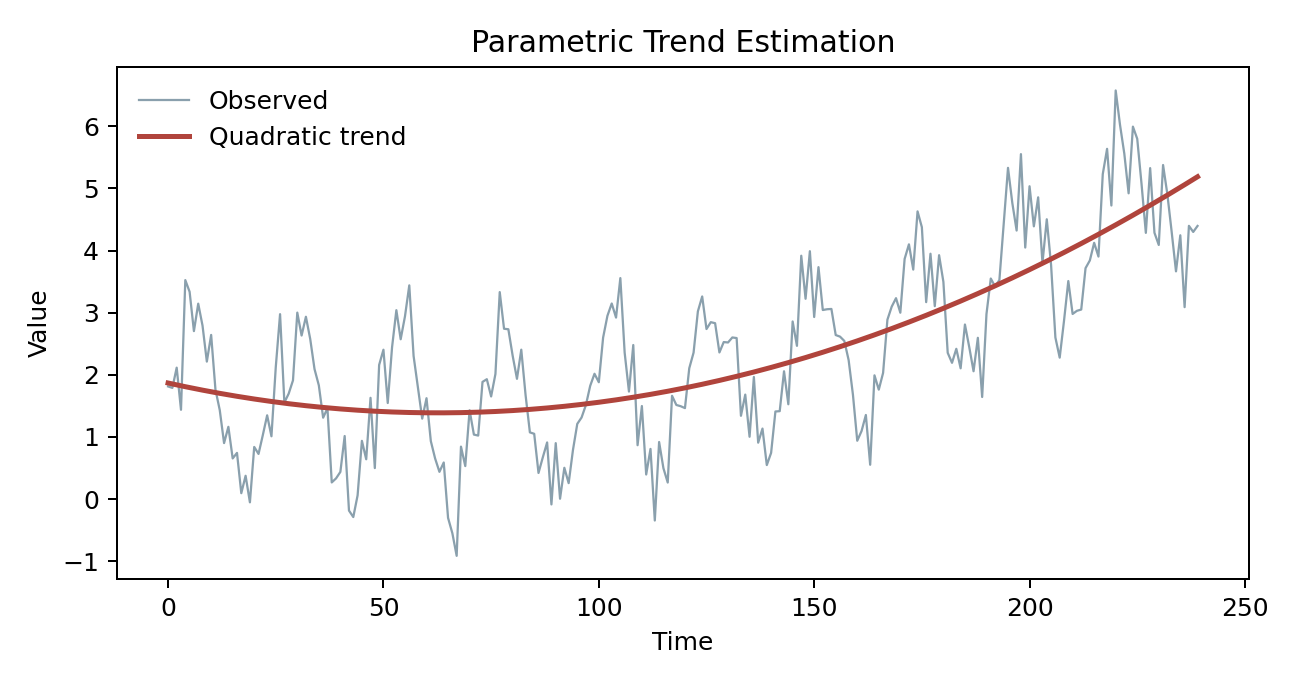
\includegraphics[width=0.86\textwidth]{ch02_fig01_parametric_trend.png}
  \caption{参数趋势估计示例：对含二次趋势、季节成分和噪声的序列拟合二次趋势。}
\end{figure}

\begin{figure}[htbp]
  \centering
  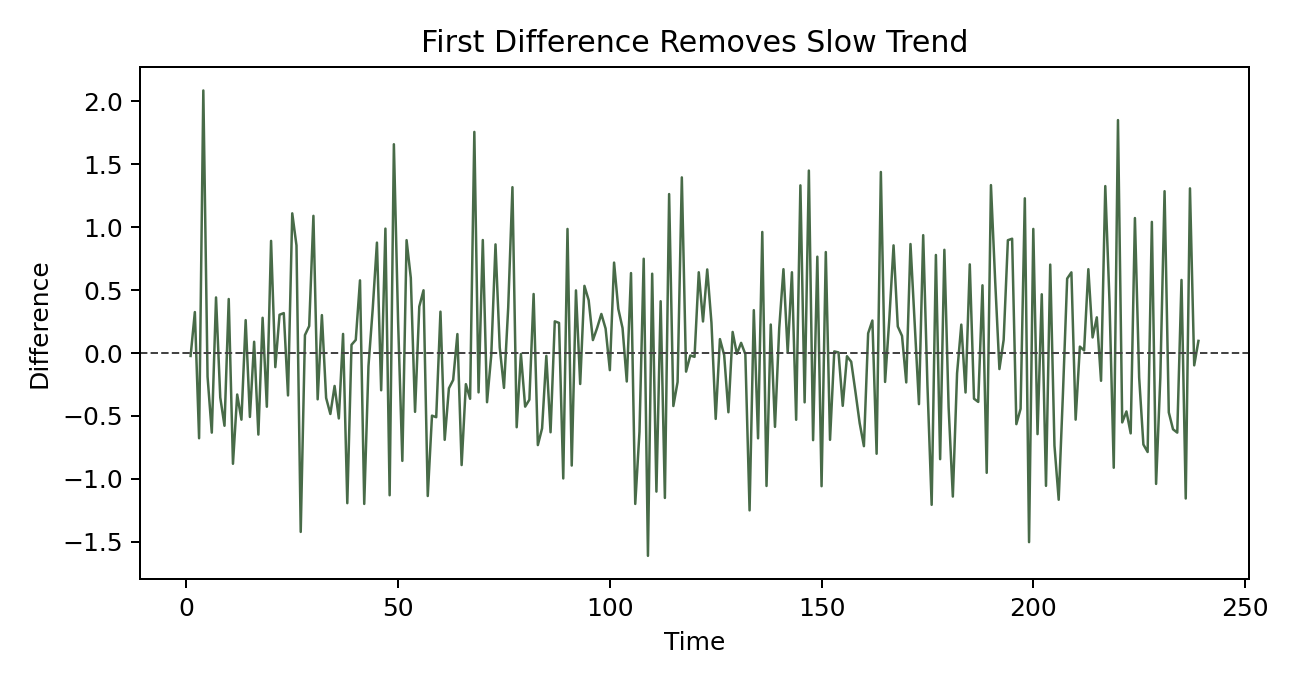
\includegraphics[width=0.86\textwidth]{ch02_fig02_differencing.png}
  \caption{一阶差分示例：差分削弱慢趋势，但也会改变噪声的依赖结构。}
\end{figure}

\begin{figure}[htbp]
  \centering
  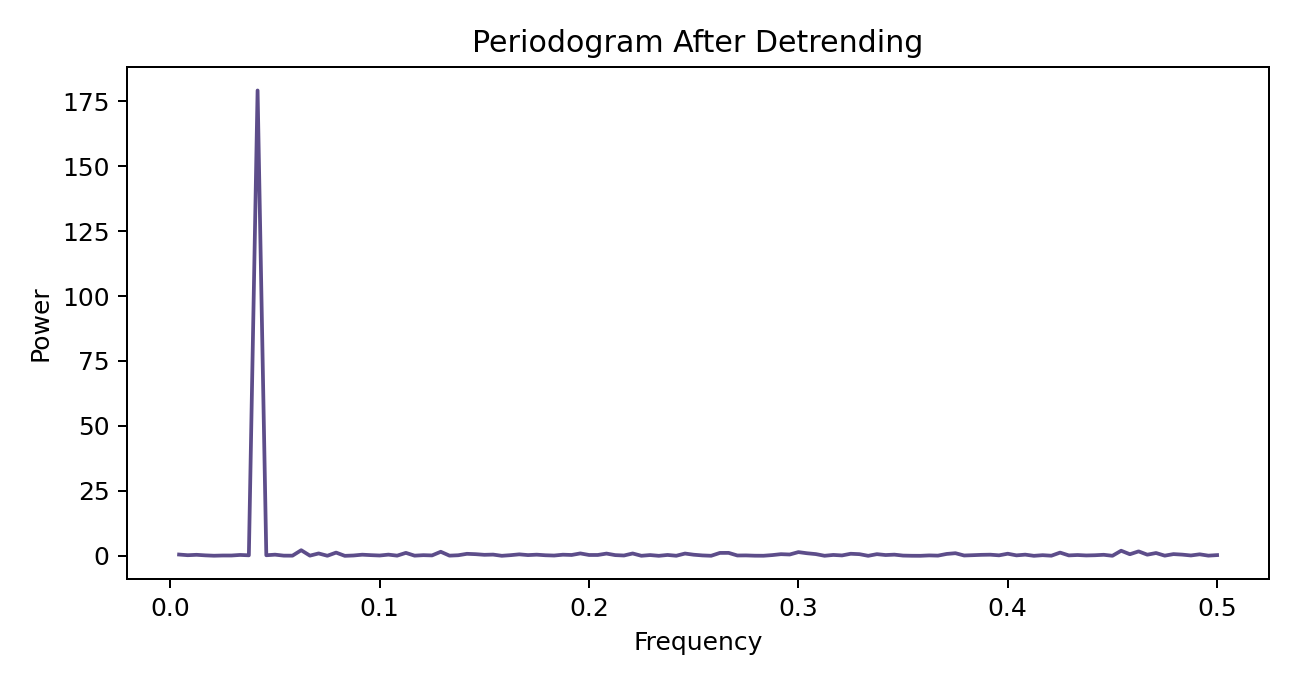
\includegraphics[width=0.86\textwidth]{ch02_fig03_periodogram.png}
  \caption{周期图示例：去除趋势后，用周期图观察残差中的周期能量。}
\end{figure}

\section{练习提要}

原文第 2.7 节的练习围绕三类任务展开：
\begin{itemize}
  \item 通过模拟和作图理解 Fourier 变换与周期图；
  \item 推导周期图在简单周期信号下的峰值位置；
  \item 反复模拟含周期信号的模型，研究样本量、噪声强度和相关噪声对周期估计的影响。
\end{itemize}
讲义使用时，可把每道练习继续拆成中文题面、公式提示和 Python 解答，作为课堂作业或附加讲解材料。

\section*{本章小结}

第 2 章把时间序列中的趋势分成几种处理方式：如果趋势形状已知，可用参数回归或非线性最小二乘；如果只知道趋势平滑，可用滚动窗口或筛估计；如果希望消去趋势，可做差分；如果趋势或信号具有周期性，可借助 Fourier 变换和周期图。需要始终记住的是：趋势、周期和相关噪声在有限样本图形中可能非常相似，因此建模假设、残差诊断和频域分析应结合使用。

\clearpage
% Source: chapters/ch03_stationary_time_series/第03章_Stationary_Time_Series_平稳时间序列.tex
\chapter{Stationary Time Series / 平稳时间序列}
\section*{本章学习目标}

本章按照原文 \textit{Stationary Time Series} 的小节顺序整理，保留主要定义、定理、模型公式和练习方向，并将原文中的 R 实践思路改写为 Python 工程实践。

完成本章后，应能够：
\begin{itemize}
  \item 复习期望、协方差、渐近阶 \(O(\cdot)\) 与 \(o(\cdot)\) 等预备知识；
  \item 形式化定义时间序列并理解有限维分布；
  \item 推导相关序列下样本均值的方差和标准误；
  \item 区分严格平稳、二阶平稳和遍历性；
  \item 判断一个序列或函数能否作为合法协方差。
\end{itemize}

\section{预备知识}

原文先复习本课程反复使用的概率记号。若 \(X\) 是随机变量，期望写作 \(E(X)\)；若 \(X,Y\) 二阶矩存在，协方差为
\[
  \mathrm{cov}(X,Y)=E\{(X-E X)(Y-E Y)\}.
\]
若 \(a_n/b_n\) 有界，则 \(a_n=O(b_n)\)；若 \(a_n/b_n\to0\)，则 \(a_n=o(b_n)\)。这些记号用于描述估计误差、协方差衰减和渐近方差的阶。

\subsection{时间序列的形式化定义}

时间序列是定义在同一概率空间上的一族随机变量
\[
  \{X_t:t\in\mathbb Z\}.
\]
实际观测通常只是有限片段 \(X_1,\ldots,X_n\)，但理论上把过程延拓到整数时间轴可使平移、滞后和协方差函数的定义更自然。

\section{样本均值及其标准误}

样本均值为
\[
  \bar X_n=\frac1n\sum_{t=1}^n X_t.
\]
在独立同分布情形，
\[
  \mathrm{var}(\bar X_n)=\frac{\sigma^2}{n}.
\]
但若序列相关，方差变为
\[
  \mathrm{var}(\bar X_n)
  =\frac1{n^2}\sum_{s=1}^n\sum_{t=1}^n\mathrm{cov}(X_s,X_t).
\]
若过程二阶平稳，记 \(c(r)=\mathrm{cov}(X_t,X_{t+r})\)，则
\[
  \mathrm{var}(\bar X_n)
  =\frac1n c(0)+\frac2{n^2}\sum_{r=1}^{n-1}(n-r)c(r).
\]
这正是时间序列推断区别于 iid 推断的第一条主线：相关性改变标准误。

\subsection{线性回归估计量的方差}

在回归模型中，若误差相关，普通最小二乘估计量的方差不再只是 \(\sigma^2(X'X)^{-1}\)。原文用该例说明：在时间序列回归中，即使估计量形式仍是最小二乘，标准误也必须反映误差的协方差矩阵。

\section{平稳过程}

\subsection{平稳性的类型}

\begin{definition}[严格平稳，原文 Definition 3.3.1]
若对任意 \(k\)、任意时间点 \(t_1,\ldots,t_k\) 和任意整数平移 \(h\)，随机向量
\[
  (X_{t_1},\ldots,X_{t_k})
\]
与
\[
  (X_{t_1+h},\ldots,X_{t_k+h})
\]
具有相同联合分布，则称 \(\{X_t\}\) 严格平稳。
\end{definition}

\begin{definition}[二阶平稳或弱平稳，原文 Definition 3.3.2]
若 \(E(X_t)=\mu\) 不随 \(t\) 变化，且
\[
  \mathrm{cov}(X_t,X_s)=c(t-s)
\]
只依赖滞后 \(t-s\)，则称 \(\{X_t\}\) 二阶平稳。
\end{definition}

严格平稳关注所有有限维分布；二阶平稳只关注一阶矩和二阶矩。若严格平稳且二阶矩有限，则自动二阶平稳。

\begin{example}[二阶平稳下样本均值方差]
若 \(\sum_{r=-\infty}^{\infty}|c(r)|<\infty\)，则
\[
  n\,\mathrm{var}(\bar X_n)
  \to \sum_{r=-\infty}^{\infty}c(r).
\]
右端称为长期方差，是后续 HAC/Newey-West 标准误的理论来源。
\end{example}

\begin{definition}[遍历性，原文 Definition 3.3.3]
粗略地说，遍历性保证时间平均可代表总体平均。若
\[
  \frac1n\sum_{t=1}^n X_t \xrightarrow{a.s.} E(X_0),
\]
则样本路径上的长期平均具有统计意义。
\end{definition}

\section{什么样的函数可以作为协方差}

\begin{definition}[非负定序列，原文 Definition 3.4.1]
序列 \(\{c(k):k\in\mathbb Z\}\) 非负定，是指对任意 \(n\) 和任意实数 \(a_1,\ldots,a_n\)，
\[
  \sum_{i=1}^n\sum_{j=1}^n a_i a_j c(i-j)\ge0.
\]
\end{definition}

\begin{theorem}[协方差的必要性质，原文 Theorem 3.4.1]
若 \(\{X_t\}\) 是离散时间二阶平稳过程，则其协方差函数 \(c(k)\) 必为非负定序列；连续时间情形中，协方差函数也必须满足对应的非负定条件。
\end{theorem}

\begin{theorem}[Fourier 判别，原文 Theorem 3.4.2]
若 \(\sum_k |c(k)|<\infty\)，则 \(c(k)\) 是合法协方差序列的一个充分条件是其 Fourier 变换
\[
  f(\omega)=\frac1{2\pi}\sum_{k=-\infty}^{\infty}c(k)e^{-ik\omega}
\]
非负。该函数就是谱密度。
\end{theorem}

\section{空间协方差}

原文最后把一维时间协方差推广到空间协方差 \(c:\mathbb R^d\to\mathbb R\)。若协方差只依赖距离 \(\|u\|\)，称为各向同性协方差。空间部分为后续理解非时间索引随机场提供背景。

\begin{lemma}[样本均值长期方差补充]
若 \(\sum_k|c(k)|<\infty\)，则
\[
  n\,\mathrm{var}(\bar X_n)
  \to \sum_{k=-\infty}^{\infty}c(k).
\]
该结论是第 8 章均值估计和 Newey-West 标准误的直接动机。
\end{lemma}

Exercise 3.1 练习协方差展开；Exercise 3.2 要求判断二阶平稳；Exercise 3.3 绘制温度数据 ACF；Exercise 3.4 连接严格平稳和函数变换；Exercise 3.5--3.6 检查给定序列或函数是否为合法协方差。

\section{Python 工程实践}

在本章目录下运行：
\begin{lstlisting}[language=bash]
python scripts/ch03_generate_figures.py
\end{lstlisting}

脚本会把图像写入本章 \texttt{figures/} 目录。当前图像用于配合本章核心概念的仿真说明；若后续补齐原始数据文件，可把模拟数据替换为原文真实数据案例。

\begin{figure}[htbp]
  \centering
  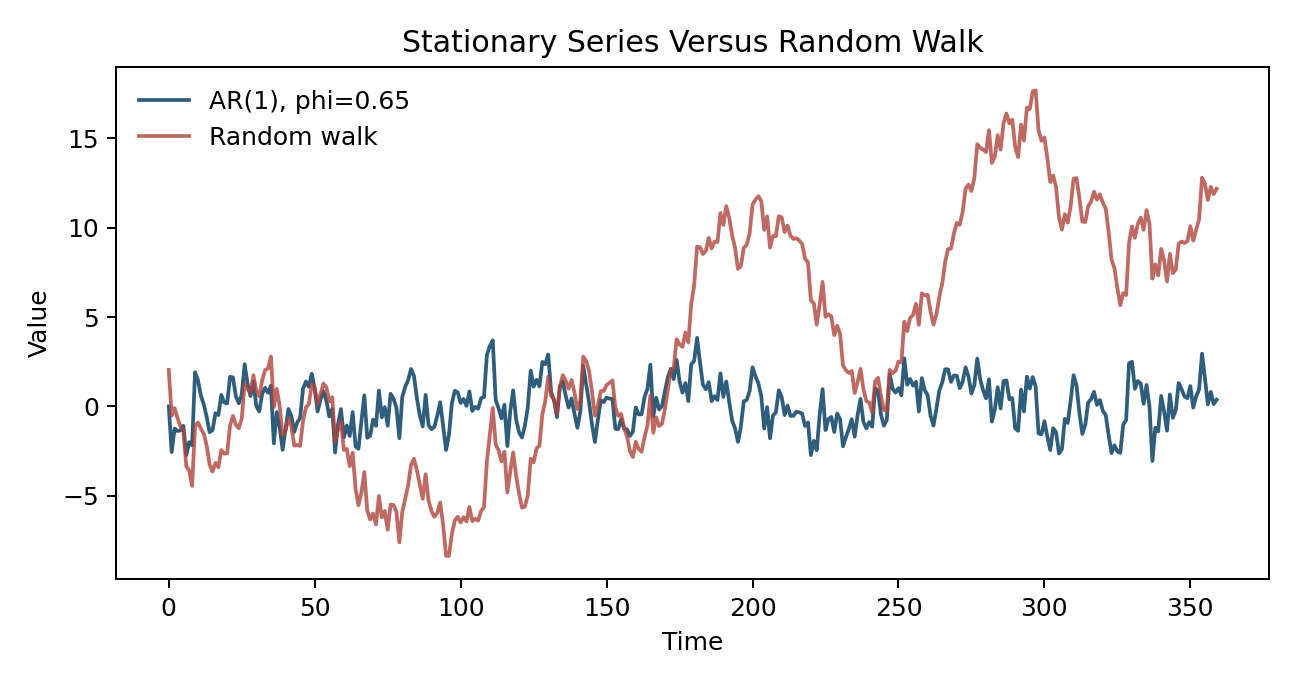
\includegraphics[width=0.86\textwidth]{ch03_fig01_stationary_vs_random_walk.png}
  \caption{平稳 AR(1) 与随机游走对比：平稳序列围绕固定均值波动，随机游走的水平随时间漂移。}
\end{figure}

\begin{figure}[htbp]
  \centering
  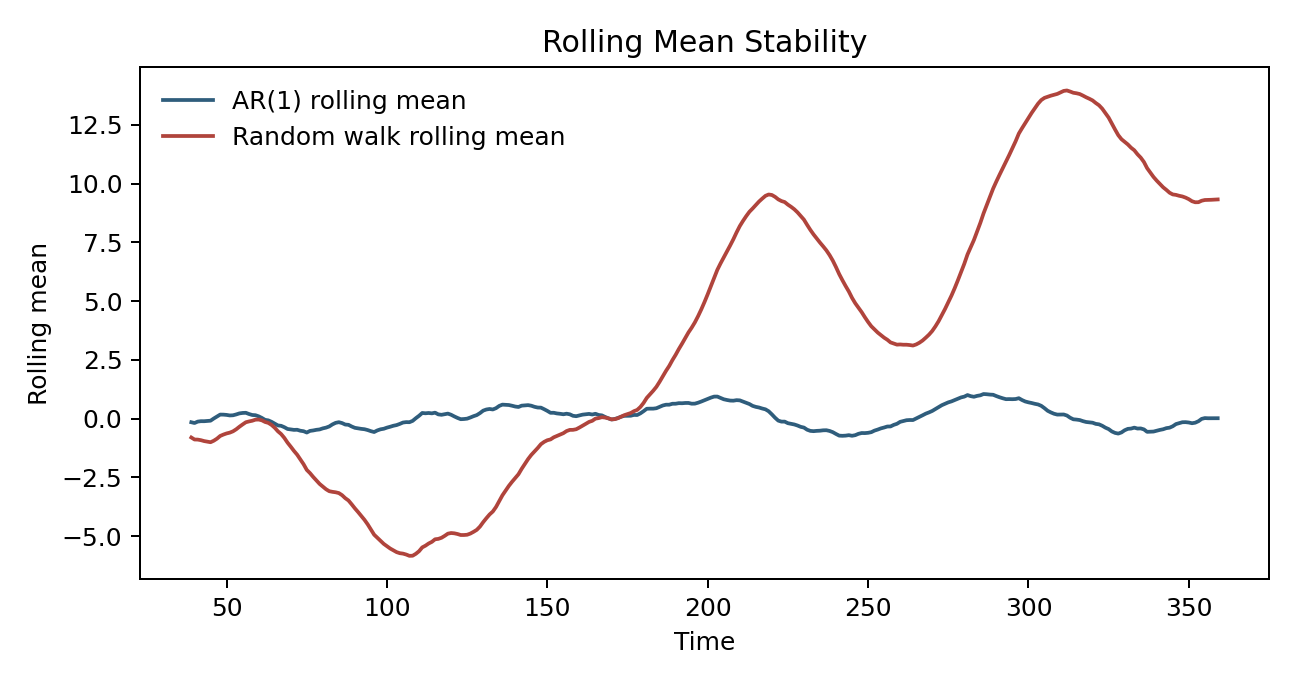
\includegraphics[width=0.86\textwidth]{ch03_fig02_rolling_mean.png}
  \caption{滚动均值稳定性：平稳序列的滚动均值较稳定，随机游走的滚动均值呈持续漂移。}
\end{figure}

\section{练习提要}

原文练习主要围绕下列方向展开：
\begin{itemize}
  \item 计算由白噪声构造的线性组合的协方差，练习协方差展开；
  \item 判断给定过程是否二阶平稳，并解释均值和协方差是否随时间改变；
  \item 为 SOI、太阳黑子和温度数据绘制 ACF，理解样本自相关的含义；
  \item 判断给定序列或函数是否可作为协方差。
\end{itemize}

\section*{本章小结}

第 3 章建立了全书的概率基础：时间序列推断依赖平稳性、遍历性和协方差结构。样本均值的标准误不再只由 \(c(0)\) 决定，而由所有滞后协方差共同决定；合法协方差必须满足非负定性，并可通过谱密度刻画。

\clearpage
% Source: chapters/ch04_linear_time_series/第04章_Linear_time_series_线性时间序列.tex
\chapter{Linear time series / 线性时间序列}
\section*{本章学习目标}

本章按照原文 \textit{Linear time series} 的小节顺序整理，保留主要定义、定理、模型公式和练习方向，并将原文中的 R 实践思路改写为 Python 工程实践。

完成本章后，应能够：
\begin{itemize}
  \item 理解线性过程和 \(MA(\infty)\) 表示；
  \item 掌握后移算子、AR(p) 差分方程和因果解；
  \item 说明 AR(2) 的伪周期现象和季节 AR 模型；
  \item 区分 AR、MA、ARMA 的因果性与可逆性；
  \item 理解单位根、非可逆过程以及 ACF/PACF 诊断。
\end{itemize}

\section{动机}

线性时间序列把当前观测表示为过去冲击的线性组合。它是全书的工作马模型：既能产生丰富的相关结构，又有清晰的协方差、预测和频域公式。

\section{线性过程与移动平均模型}

\begin{definition}[线性过程与 \(MA(\infty)\)，原文 Definition 4.2.1]
若 \(\{\varepsilon_t\}\) 是均值为 0、方差为 \(\sigma^2\) 的不相关创新，且
\[
  X_t=\sum_{j=0}^{\infty}\psi_j\varepsilon_{t-j},
  \qquad \sum_{j=0}^{\infty}|\psi_j|<\infty,
\]
则称 \(\{X_t\}\) 是线性过程，也称具有 \(MA(\infty)\) 表示。
\end{definition}

\begin{lemma}[无限和的存在性，原文 Lemma 4.2.1]
若系数满足适当可和条件且创新二阶矩有限，则上述无限和在均方意义下存在，并定义一个二阶平稳过程。
\end{lemma}

其均值为 0，自协方差为
\[
  c(k)=\sigma^2\sum_{j=0}^{\infty}\psi_j\psi_{j+|k|}.
\]

\section{AR(p) 模型}

\subsection{差分方程与后移算子}

后移算子定义为 \(BX_t=X_{t-1}\)。AR(p) 模型写作
\[
  X_t=\phi_1X_{t-1}+\cdots+\phi_pX_{t-p}+\varepsilon_t,
\]
或
\[
  \phi(B)X_t=\varepsilon_t,\qquad
  \phi(z)=1-\phi_1z-\cdots-\phi_pz^p.
\]

\subsection{AR(1) 的两个解}

对
\[
  X_t=\phi X_{t-1}+\varepsilon_t,
\]
若 \(|\phi|<1\)，因果平稳解为
\[
  X_t=\sum_{j=0}^{\infty}\phi^j\varepsilon_{t-j}.
\]
若 \(|\phi|>1\)，也可构造非因果平稳解
\[
  X_t=-\sum_{j=1}^{\infty}\phi^{-j}\varepsilon_{t+j},
\]
但该解依赖未来创新，不适合作为预测模型。

\begin{lemma}[AR(p) 因果解，原文 Lemma 4.3.1]
若 \(\phi(z)\) 的所有根都在单位圆外，则 AR(p) 有唯一因果平稳解，且可写成
\[
  X_t=\sum_{j=0}^{\infty}\psi_j\varepsilon_{t-j},
\]
其中 \(\psi(z)=1/\phi(z)\) 在单位圆附近解析。
\end{lemma}

\section{AR(2)、伪周期与季节自回归}

AR(2) 的特征根若为复数，会产生阻尼振荡。若根可表示为 \(re^{\pm i\omega}\)，则样本路径和自协方差常表现出近似周期
\[
  P=\frac{2\pi}{\omega}.
\]
这就是原文称为 pseudo periodicity 的现象：模型没有确定性周期项，但相关结构会产生类似周期的波动。

季节自回归模型把滞后设为季节长度，例如月度数据中常见
\[
  X_t=\Phi X_{t-12}+\varepsilon_t.
\]
它用于刻画每年同月之间的相关性。

\section{ARMA 模型}

\begin{definition}[AR、ARMA 与 MA，原文 Definition 4.5.1]
ARMA(p,q) 模型定义为
\[
  \phi(B)X_t=\theta(B)\varepsilon_t,
\]
其中
\[
  \phi(z)=1-\phi_1z-\cdots-\phi_pz^p,\qquad
  \theta(z)=1+\theta_1z+\cdots+\theta_qz^q.
\]
当 \(q=0\) 时为 AR(p)，当 \(p=0\) 时为 MA(q)。
\end{definition}

\begin{definition}[因果与可逆，原文 Definition 4.5.2]
若 \(\phi(z)\) 的根都在单位圆外，则模型因果；若 \(\theta(z)\) 的根都在单位圆外，则模型可逆。可逆性保证创新可由当前和过去观测恢复：
\[
  \varepsilon_t=\sum_{j=0}^{\infty}\pi_j X_{t-j}.
\]
\end{definition}

\section{ARFIMA、单位根与诊断}

ARFIMA 模型通过分数差分 \((1-B)^d\) 描述长记忆。单位根模型含有 \(\phi(1)=0\)，最典型例子是随机游走
\[
  X_t=X_{t-1}+\varepsilon_t.
\]
诊断上，MA(q) 的 ACF 通常 q 阶截尾，AR(p) 的 PACF 通常 p 阶截尾；单位根过程的 ACF 衰减很慢，差分后更接近平稳。

\section{原文小节覆盖补充}

\subsection{无限随机变量和}
原文在定义线性过程前先处理无限随机变量和的收敛问题。若 \(\sum_jE|a_j\varepsilon_{t-j}|^2<\infty\)，则部分和在均方意义下收敛；这保证 \(MA(\infty)\) 表示真正定义了随机变量。

\begin{example}[原文 Example 4.2.1]
若 \(\{X_t\}\) 严格平稳且方差有限，定义 \(Y_t=\sum_{j=0}^{\infty}a_jX_{t-j}\)，则在系数足够可和时，\(Y_t\) 也是良好定义的平稳线性滤波序列。
\end{example}

\subsection{两个 AR(1) 解和一般 AR(p) 解}
同一个 AR 方程可能有因果解和非因果解。因果解依赖过去创新，适合预测；非因果解依赖未来创新，通常只作为理论对照。Exercise 4.1 要求求 AR(1) 平稳解；Exercise 4.2 要求处理一般 AR(p) 表示。

\begin{lemma}[解析函数技术，原文 Lemma 4.3.2--4.3.3]
若 \(\phi(z)\) 在单位圆附近无零点，则 \(1/\phi(z)\) 可展开为收敛幂级数，因此 AR(p) 可写成 \(MA(\infty)\)。
\end{lemma}

\subsection{AR(2) 显式解、伪周期和周期图历史}
AR(2) 是展示阻尼振荡的最小模型。若特征根为复共轭，样本路径和 ACF 呈现伪周期。Exercise 4.3、Exercise 4.4、Exercise 4.5 和 Exercise 4.6 都围绕 AR(2) 因果条件、显式解和指定伪周期展开。

\begin{example}[伪周期 AR(2)]
当根为 \(re^{\pm i\omega}\) 时，自协方差含有 \(\cos(k\omega)\) 型项，周期近似为 \(2\pi/\omega\)。
\end{example}

\subsection{季节 AR、AR(\(\infty\)) 与模拟}
季节 AR 使用季节滞后，例如 \(X_t=\Phi X_{t-12}+\varepsilon_t\)。AR(\(\infty\)) 仍依赖系数可和和解析性。原文模拟部分强调，给定创新、初始值和递推公式即可生成 AR 样本；Exercise 4.7 要求用非高斯创新模拟。

\subsection{ARMA、ARFIMA、单位根、非可逆和诊断}
ARMA 综合 AR 的递推依赖与 MA 的冲击叠加；ARFIMA 用分数差分描述长记忆；单位根过程需要差分；非可逆 MA 虽可能有相同 ACF，但创新不能由过去观测稳定恢复。诊断部分强调 ACF/PACF 和单位根检查。

\subsection{4.8 模型模拟}
原文第 4.8 节把 AR、MA、ARMA、单位根模型的模拟统一为“生成创新后递推或滤波”。模拟用于理解样本路径、验证 ACF/PACF 诊断，也用于构造课堂实验。

\subsection{4.10 附录}
附录补充若干代数推导，帮助读者从特征根、多项式和递推公式之间来回转换。它不引入新模型，但支撑正文中 AR 解和 ARMA 表示的推导。

\section{Python 工程实践}

在本章目录下运行：
\begin{lstlisting}[language=bash]
python scripts/ch04_generate_figures.py
\end{lstlisting}

脚本会把图像写入本章 \texttt{figures/} 目录。当前图像用于配合本章核心概念的仿真说明；若后续补齐原始数据文件，可把模拟数据替换为原文真实数据案例。

\begin{figure}[htbp]
  \centering
  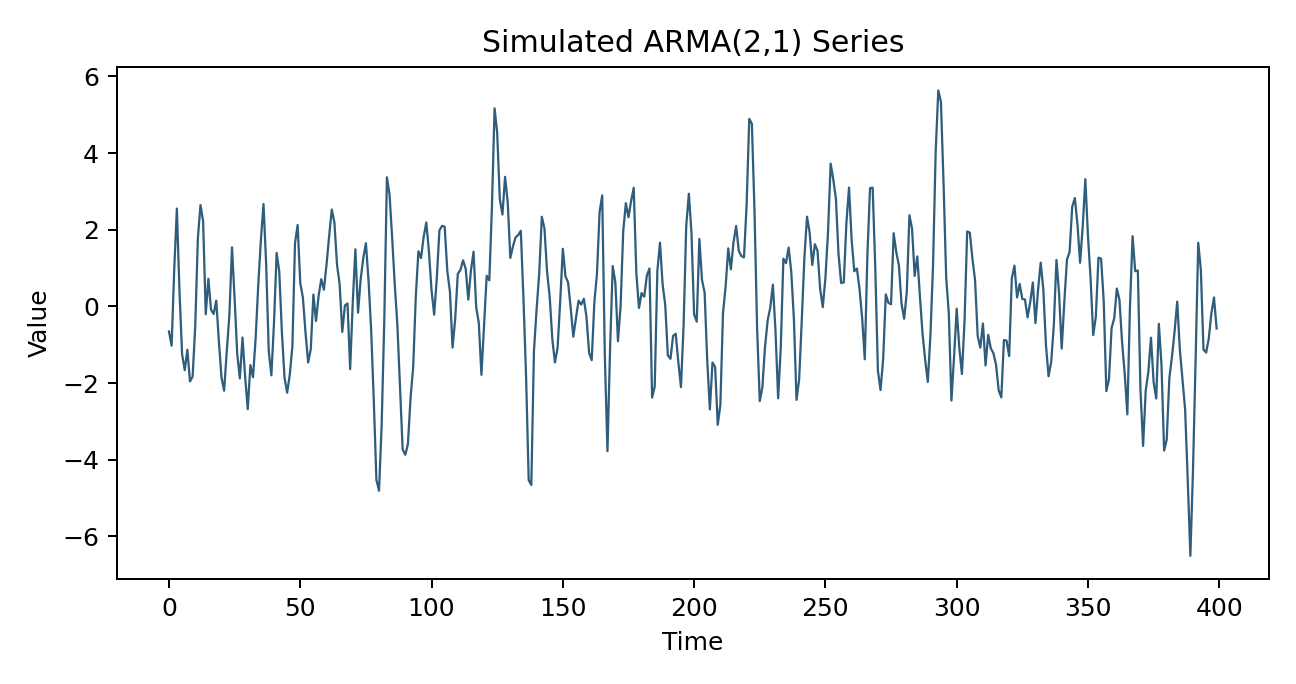
\includegraphics[width=0.86\textwidth]{ch04_fig01_arma_series.png}
  \caption{模拟 ARMA(2,1) 序列：线性模型可产生持续相关但均值稳定的波动。}
\end{figure}

\begin{figure}[htbp]
  \centering
  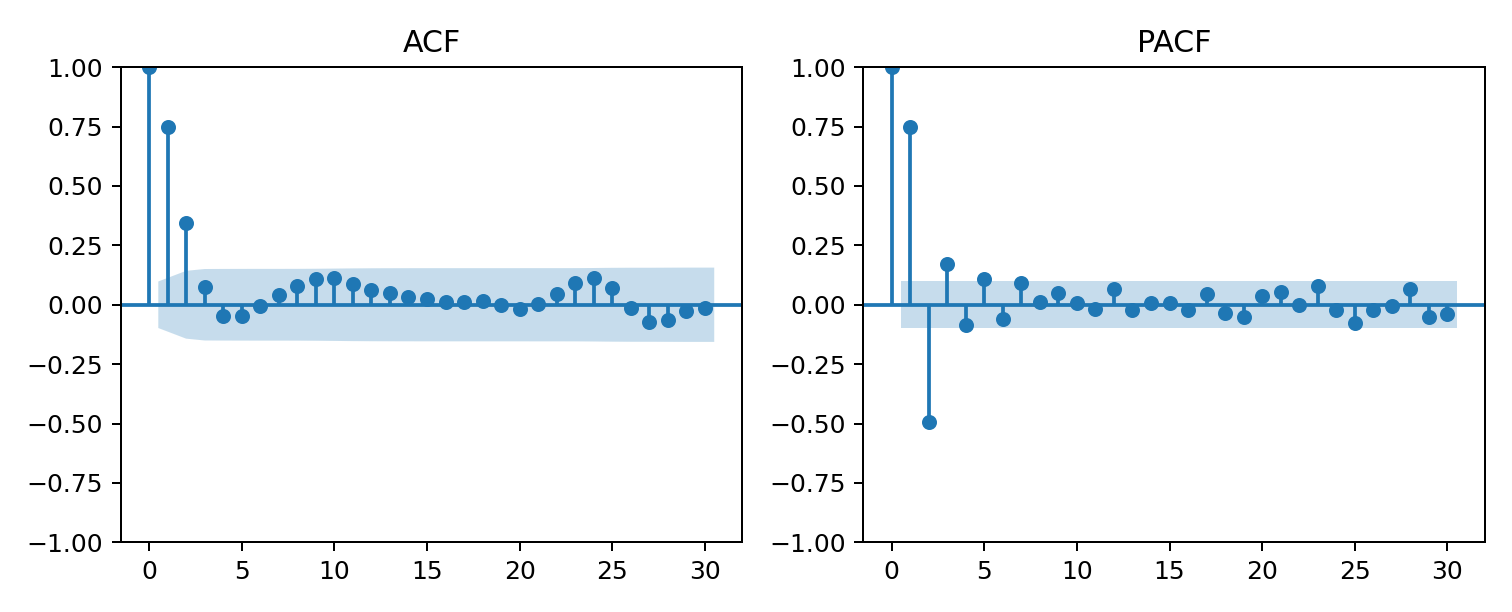
\includegraphics[width=0.86\textwidth]{ch04_fig02_acf_pacf.png}
  \caption{ACF/PACF 诊断图：用于区分 AR 与 MA 结构并辅助阶数选择。}
\end{figure}

\section{练习提要}

原文练习主要围绕下列方向展开：
\begin{itemize}
  \item 求 AR(1)、AR(2) 的平稳因果解；
  \item 根据特征根判断 AR(p) 的因果性；
  \item 构造具有指定伪周期的 AR(2) 模型；
  \item 模拟 ARMA、单位根和非可逆模型并比较 ACF/PACF。
\end{itemize}

\section*{本章小结}

第 4 章给出了线性时间序列的模型语言。后移算子把差分方程写成多项式，根的位置决定因果性、可逆性和单位根；ACF 与 PACF 则把这些理论结构变成可观察诊断。

\clearpage
% Source: chapters/ch05_a_review_of_some_results_from_multivariate_a/第05章_Multivariate_analysis_review_多元分析结果回顾.tex
\chapter{A review of some results from multivariate analysis / 多元分析结果回顾}
\section*{本章学习目标}

本章按照原文 \textit{A review of some results from multivariate analysis} 的小节顺序整理，保留主要定义、定理、模型公式和练习方向，并将原文中的 R 实践思路改写为 Python 工程实践。

完成本章后，应能够：
\begin{itemize}
  \item 复习内积、范数、正交和投影；
  \item 把线性预测理解为 Hilbert 空间投影；
  \item 推导多阶段投影和偏相关；
  \item 理解精度矩阵中的零元素与条件不相关的关系；
  \item 为后续 Durbin-Levinson 和部分自相关建立几何语言。
\end{itemize}

\section{欧氏空间与投影}

\subsection{内积、范数与正交}

在 \(\mathbb R^n\) 中，内积为
\[
  \langle x,y\rangle=\sum_{i=1}^n x_i y_i,
\]
范数为 \(\|x\|=\sqrt{\langle x,x\rangle}\)。若 \(\langle x,y\rangle=0\)，称 \(x\) 与 \(y\) 正交。

\subsection{投影}

把向量 \(Y\) 投影到由 \(X\) 张成的空间，得到
\[
  \hat Y=\alpha X,\qquad
  \alpha=\frac{\langle Y,X\rangle}{\langle X,X\rangle}.
\]
残差 \(Y-\hat Y\) 与 \(X\) 正交。多元情形中，若 \(X\) 为设计矩阵，则
\[
  \hat Y=X(X'X)^{-1}X'Y.
\]
投影矩阵 \(P=X(X'X)^{-1}X'\) 满足 \(P^2=P\) 和 \(P'=P\)。

\subsection{多阶段投影}

若先投影到一个子空间，再对残差投影到另一个正交补空间，可以把复杂预测分解为几个正交部分。这一思想在后续部分自相关和 Durbin-Levinson 递推中反复出现。

\section{随机变量空间}

二阶随机变量构成一个带内积的空间：
\[
  \langle X,Y\rangle=E(XY).
\]
若使用中心化随机变量，则内积对应协方差：
\[
  \langle X-E X,Y-EY\rangle=\mathrm{cov}(X,Y).
\]
因此，最佳线性预测就是在随机变量空间中的正交投影。

\section{线性预测}

设要用 \(X_1,\ldots,X_p\) 线性预测 \(Y\)，预测量为
\[
  \hat Y=\sum_{j=1}^p a_jX_j.
\]
最优系数由正交方程给出：
\[
  E\left[(Y-\hat Y)X_k\right]=0,\qquad k=1,\ldots,p.
\]
写成矩阵形式：
\[
  \Gamma a=\gamma,
\]
其中 \(\Gamma_{ij}=E(X_iX_j)\)，\(\gamma_i=E(YX_i)\)。

\section{偏相关}

偏相关衡量在控制其他变量后两个变量之间剩余的线性关系。设 \(X\) 与 \(Y\) 都先对 \(Z\) 做线性投影，残差分别为
\[
  X^\perp=X-\mathrm{Proj}(X\mid Z),\qquad
  Y^\perp=Y-\mathrm{Proj}(Y\mid Z).
\]
则偏相关为
\[
  \rho_{XY\cdot Z}
  =\frac{\mathrm{cov}(X^\perp,Y^\perp)}
  {\sqrt{\mathrm{var}(X^\perp)\mathrm{var}(Y^\perp)}}.
\]
在时间序列中，部分自相关就是 \(X_t\) 与 \(X_{t+h}\) 在控制中间 \(X_{t+1},\ldots,X_{t+h-1}\) 后的相关。

\section{精度矩阵性质}

协方差矩阵 \(\Sigma\) 的逆矩阵
\[
  \Omega=\Sigma^{-1}
\]
称为精度矩阵。若随机向量为高斯分布，则 \(\Omega_{ij}=0\) 等价于第 \(i\) 与第 \(j\) 个分量在给定其他分量后条件独立。即使非高斯，精度矩阵的零元素也对应线性条件不相关结构。

\section{附录：Hilbert 空间投影}

原文附录把投影定理放在 Hilbert 空间中陈述：若 \(\mathcal M\) 是闭线性子空间，则任意 \(Y\) 可唯一分解为
\[
  Y=\mathrm{Proj}_{\mathcal M}Y+e,
  \qquad e\perp \mathcal M.
\]
该定理是预测理论的几何基础。

\section{原文例题与定义补充}

\begin{example}[原文 Example 5.3.1：三个随机向量]
原文构造 \(X_1,X_2,X_3\) 三个随机向量，用来说明普通相关和偏相关可能给出不同结论。即使 \(X_1\) 与 \(X_2\) 有相关性，在控制 \(X_3\) 后二者的残差相关也可能消失。
\end{example}

\begin{definition}[原文 Definition 5.5.1：投影]
随机变量 \(Y\) 到由 \(X_1,\ldots,X_p\) 张成空间的投影，是该空间中使均方误差
\[
  E(Y-\hat Y)^2
\]
最小的元素 \(\hat Y\)。残差 \(Y-\hat Y\) 与所有解释变量正交。
\end{definition}

\begin{example}[原文 Example 5.5.1：Hilbert 空间]
\(\mathbb R^n\) 是有限维 Hilbert 空间；二阶随机变量在内积 \(E(XY)\) 下也形成 Hilbert 空间。预测理论把这两个例子统一起来。
\end{example}

第 5.4 节的证明说明，精度矩阵零元素与残差正交关系等价；第 5.5 节附录则把欧氏投影推广到闭线性子空间，为后续时间序列预测提供抽象框架。

\section{Python 工程实践}

在本章目录下运行：
\begin{lstlisting}[language=bash]
python scripts/ch05_generate_figures.py
\end{lstlisting}

脚本会把图像写入本章 \texttt{figures/} 目录。当前图像用于配合本章核心概念的仿真说明；若后续补齐原始数据文件，可把模拟数据替换为原文真实数据案例。

\begin{figure}[htbp]
  \centering
  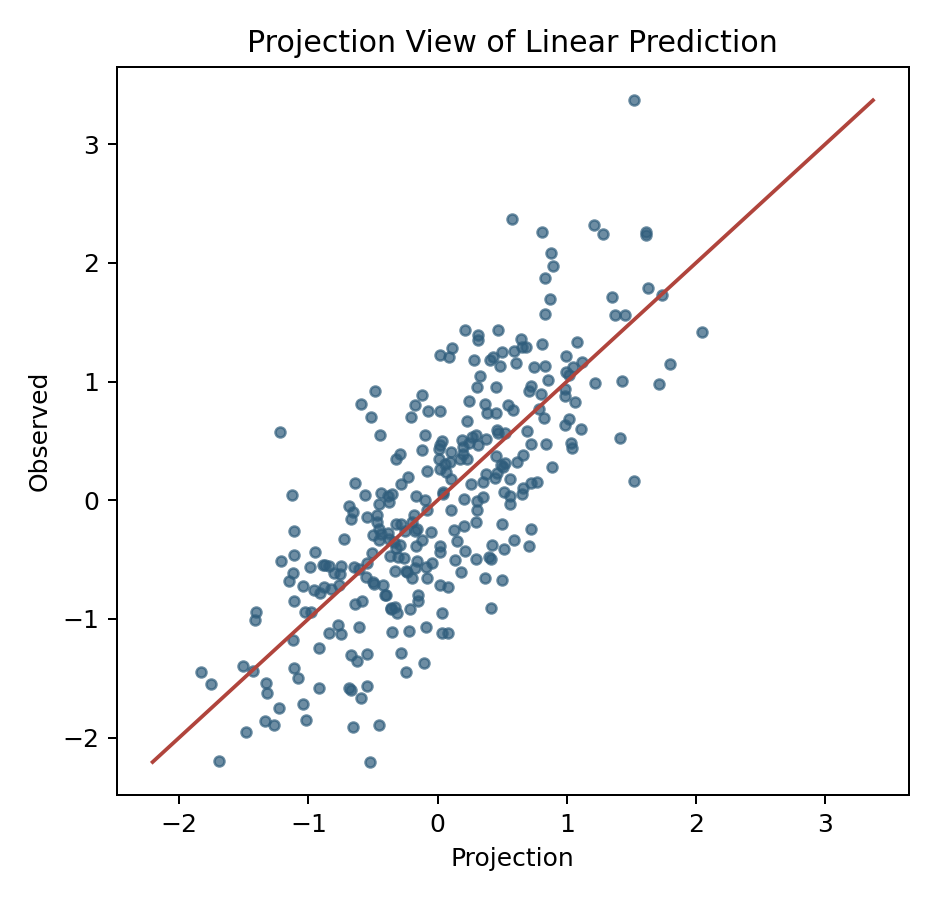
\includegraphics[width=0.86\textwidth]{ch05_fig01_projection_prediction.png}
  \caption{线性预测的投影视角：预测值是观测向解释变量空间的正交投影。}
\end{figure}

\begin{figure}[htbp]
  \centering
  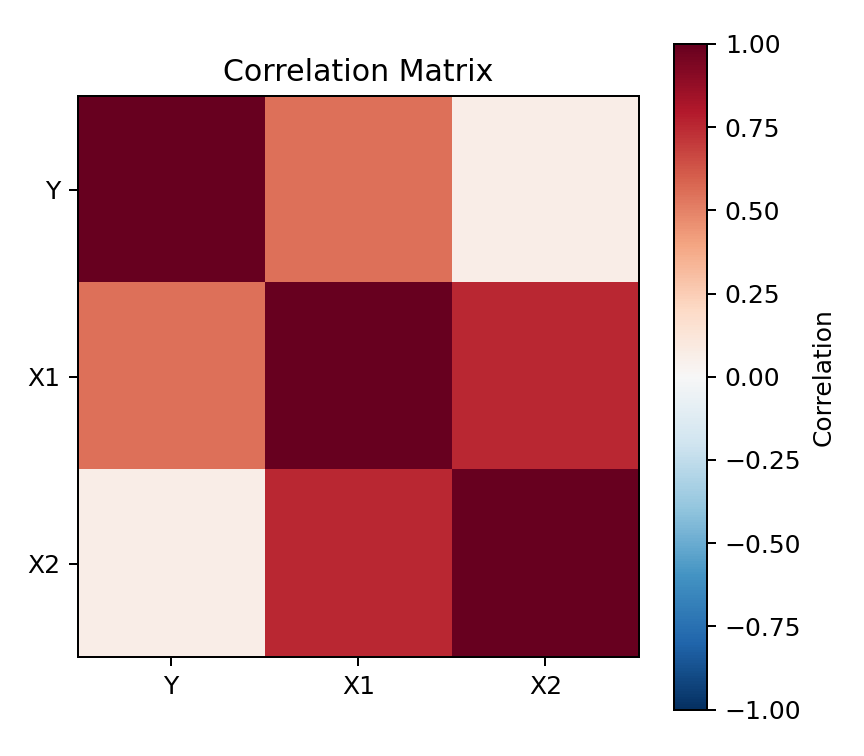
\includegraphics[width=0.86\textwidth]{ch05_fig02_correlation_matrix.png}
  \caption{相关矩阵示例：多元关系可由协方差矩阵和精度矩阵进一步分析。}
\end{figure}

\section{练习提要}

原文练习主要围绕下列方向展开：
\begin{itemize}
  \item 计算向量投影和投影残差，验证正交性；
  \item 推导最优线性预测的正规方程；
  \item 用残差相关解释偏相关；
  \item 从协方差矩阵求精度矩阵并解释零元素。
\end{itemize}

\section*{本章小结}

第 5 章把多元线性代数翻译成时间序列预测语言。投影给出最小均方误差预测，偏相关解释 PACF，精度矩阵则连接到条件依赖结构。

\clearpage
% Source: chapters/ch06_the_autocovariance_and_partial_covariance_of/第06章_Autocovariance_partial_covariance_自协方差与偏协方差.tex
\chapter{Autocovariance and partial covariance / 自协方差与偏协方差}
\section*{本章学习目标}

本章按照原文 \textit{The autocovariance and partial covariance of a stationary time series} 的小节顺序整理，保留主要定义、定理、模型公式和练习方向，并将原文中的 R 实践思路改写为 Python 工程实践。

完成本章后，应能够：
\begin{itemize}
  \item 推导线性过程、AR、MA、ARMA 的自协方差；
  \item 理解 ARMA 自协方差衰减速度；
  \item 估计样本 ACF 并识别模型；
  \item 定义时间序列偏协方差与 PACF；
  \item 理解方差矩阵、精度矩阵和非因果模型的 ACF。
\end{itemize}

\section{自协方差函数}

平稳过程的自协方差定义为
\[
  c(k)=\mathrm{cov}(X_t,X_{t+k}).
\]
对线性过程
\[
  X_t=\sum_{j=0}^{\infty}\psi_j\varepsilon_{t-j},
\]
若 \(\mathrm{var}(\varepsilon_t)=\sigma^2\)，则
\[
  c(k)=\sigma^2\sum_{j=0}^{\infty}\psi_j\psi_{j+|k|}.
\]

\begin{lemma}[线性表示的协方差，原文 Lemma 6.1.1]
若平稳序列具有绝对可和的线性表示，则其自协方差由系数卷积给出，并且 \(\sum_k|c(k)|<\infty\) 在相应条件下成立。
\end{lemma}

\subsection{ARMA 协方差的衰减}

因果可逆 ARMA 的系数通常几何衰减，因此自协方差也几何衰减。AR 根越接近单位圆，ACF 衰减越慢。

\section{AR、MA 和 ARMA 的自协方差}

AR(p) 模型
\[
  X_t=\phi_1X_{t-1}+\cdots+\phi_pX_{t-p}+\varepsilon_t
\]
两边同乘 \(X_{t-k}\) 并取期望，可得 Yule-Walker 方程：
\[
  c(k)=\phi_1c(k-1)+\cdots+\phi_pc(k-p),\qquad k\ge1.
\]
对 AR(1)，
\[
  c(k)=\frac{\sigma^2}{1-\phi^2}\phi^{|k|}.
\]

MA(q) 模型
\[
  X_t=\varepsilon_t+\theta_1\varepsilon_{t-1}+\cdots+\theta_q\varepsilon_{t-q}
\]
的自协方差在 \(q\) 阶后截尾：
\[
  c(k)=0,\qquad |k|>q.
\]
ARMA 模型的 ACF 通常在前若干阶受 MA 部分影响，随后按 AR 部分的差分方程递推衰减。

\section{从数据估计 ACF}

若均值未知，样本自协方差通常写为
\[
  \hat c(k)=\frac1n\sum_{t=1}^{n-k}(X_t-\bar X)(X_{t+k}-\bar X),
\]
样本自相关为
\[
  \hat\rho(k)=\frac{\hat c(k)}{\hat c(0)}.
\]
ACF 图是识别线性模型的基础：MA(q) 的 ACF 倾向截尾，AR(p) 的 ACF 倾向拖尾。

\section{偏相关}

\begin{definition}[偏协方差/偏相关，原文 Definition 6.2.1]
\(X_t\) 与 \(X_{t+h}\) 在控制中间变量 \(X_{t+1},\ldots,X_{t+h-1}\) 后的残差协方差称为偏协方差；标准化后称为偏相关。
\end{definition}

对平稳序列，h 阶偏自相关可记为 \(\phi_{h,h}\)。它等于用 \(X_{t-1},\ldots,X_{t-h}\) 预测 \(X_t\) 的最佳 AR(h) 模型中第 h 个系数。AR(p) 的 PACF 在 p 阶后截尾。

\section{方差矩阵、精度矩阵与非因果模型}

对向量 \(X_1,\ldots,X_n\)，协方差矩阵为 Toeplitz 形式：
\[
  \Gamma_n=(c(i-j))_{i,j=1}^n.
\]
其逆矩阵反映条件线性依赖结构。AR(p) 过程的精度矩阵具有带状结构，这对应“给定最近 p 个邻居后更远变量无直接线性影响”。

原文最后讨论非因果时间序列和 minimum phase。谱密度定义为
\[
  f(\omega)=\frac1{2\pi}\sum_{k=-\infty}^{\infty}c(k)e^{-ik\omega},
\]
不同因果/非因果表示可能具有相同的二阶结构，因此仅凭 ACF 不能总是区分时间方向。

\section{原文小节覆盖补充}

\subsection{ARMA 自协方差衰减速度}
因果 ARMA 的自协方差通常按几何速度衰减。AR 根越接近单位圆，衰减越慢；复根会导致振荡衰减。这解释了 ACF 图中拖尾和周期形态。

\subsection{AR 自协方差与 Yule-Walker 方程}
AR(p) 自协方差满足 Yule-Walker 递推。Exercise 6.1 和 Exercise 6.2 延续第 4 章 AR(2) 练习，要求推出 ACF 形状和周期。

\begin{example}[原文 \(p=2\) 例子]
若 \(\phi(z)=1-\phi_1z-\phi_2z^2\) 的根为复共轭，则 \(c(k)\) 是指数衰减和三角函数振荡的乘积。
\end{example}

\subsection{MA、ARMA 和样本 ACF}
MA(q) 的自协方差在 q 阶后截尾；ARMA(p,q) 在前 q 阶受 MA 部分影响，随后满足 AR 递推。样本 ACF 用 \(\hat c(k)/\hat c(0)\) 估计，但大滞后处不稳定。

\subsection{偏相关与 PACF 图}
偏协方差是去除中间变量线性影响后的残差协方差。h 阶 PACF 等于最佳 AR(h) 预测中最后一个系数。Exercise 6.3 研究可逆 MA(1) 的偏相关；Exercise 6.4 和 Exercise 6.5 比较 AR 与实际温度数据的 ACF/PACF。

\subsection{方差矩阵和非因果过程}
原文第 6.3 节研究 Toeplitz 方差矩阵和精度矩阵。第 6.4 节定义谱密度与 minimum phase，并讨论非因果 ARMA 的 Yule-Walker 方程和滤波。Exercise 6.6、Exercise 6.7、Exercise 6.8 分别对应 AR(2) 方差矩阵、精度矩阵性质和非因果 AR(p)。

\begin{definition}[minimum phase，原文 Definition 6.4.2]
若 ARMA 表示中 AR 和 MA 多项式的根都在单位圆外，则称该表示为 minimum phase；它对应因果且可逆的规范表示。
\end{definition}

\section{Python 工程实践}

在本章目录下运行：
\begin{lstlisting}[language=bash]
python scripts/ch06_generate_figures.py
\end{lstlisting}

脚本会把图像写入本章 \texttt{figures/} 目录。当前图像用于配合本章核心概念的仿真说明；若后续补齐原始数据文件，可把模拟数据替换为原文真实数据案例。

\begin{figure}[htbp]
  \centering
  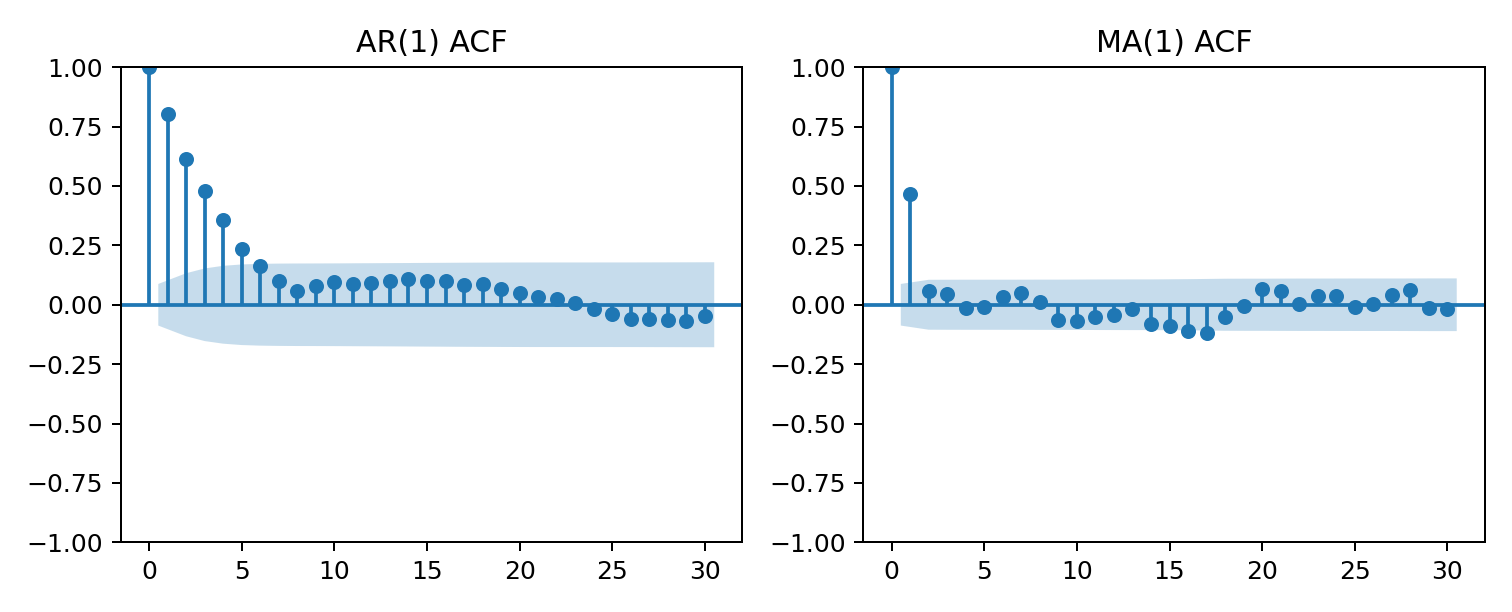
\includegraphics[width=0.86\textwidth]{ch06_fig01_acf_shapes.png}
  \caption{AR 与 MA 的 ACF 形态：AR 通常拖尾，MA 通常截尾。}
\end{figure}

\begin{figure}[htbp]
  \centering
  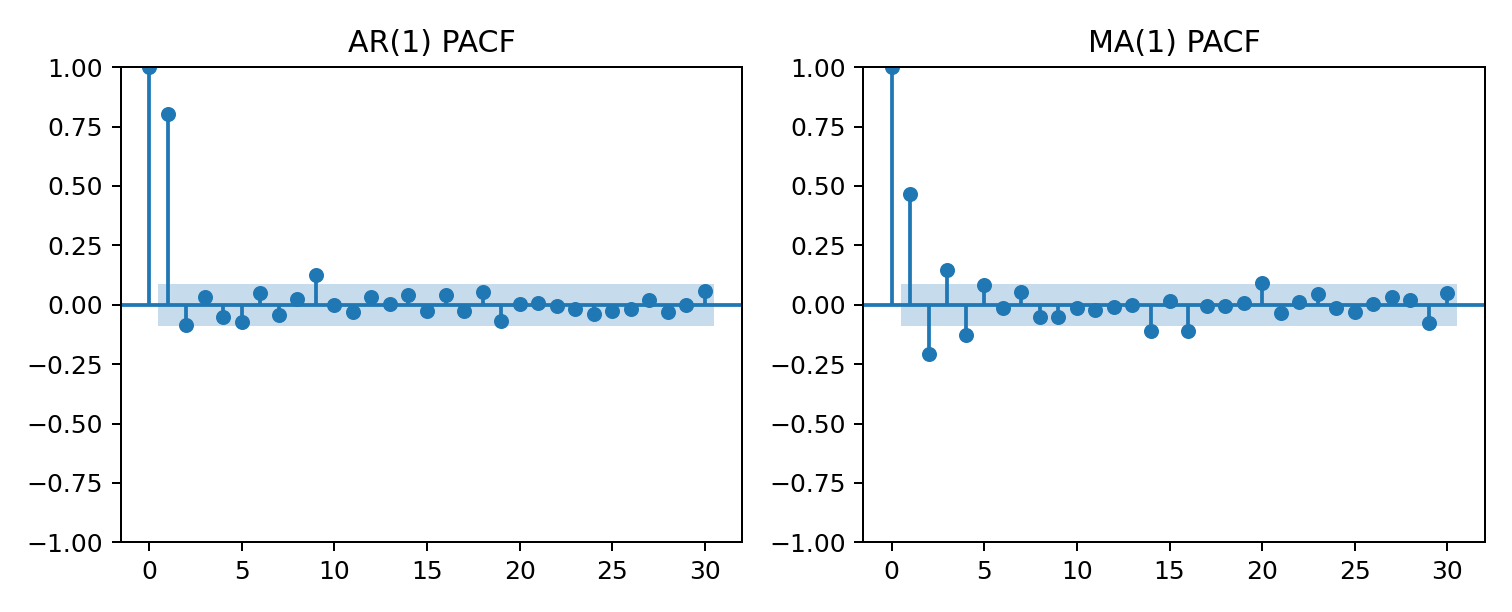
\includegraphics[width=0.86\textwidth]{ch06_fig02_pacf_shapes.png}
  \caption{AR 与 MA 的 PACF 形态：AR 通常截尾，MA 通常拖尾。}
\end{figure}

\section{练习提要}

原文练习主要围绕下列方向展开：
\begin{itemize}
  \item 推导 AR(2) 的自协方差和伪周期 ACF；
  \item 比较 AR、MA、ARMA 的 ACF/PACF 图；
  \item 计算 MA(1) 的偏相关；
  \item 证明 AR(p) 方差矩阵逆的带状结构。
\end{itemize}

\section*{本章小结}

第 6 章把线性模型与可观察的相关图联系起来。Yule-Walker 方程给出 AR 的协方差递推，MA 的协方差截尾，PACF 则将投影几何转化为模型识别工具。

\clearpage
% Source: chapters/ch07_prediction/第07章_Prediction_预测.tex
\chapter{Prediction / 预测}
\section*{本章学习目标}

本章按照原文 \textit{Prediction} 的小节顺序整理，保留主要定义、定理、模型公式和练习方向，并将原文中的 R 实践思路改写为 Python 工程实践。

完成本章后，应能够：
\begin{itemize}
  \item 理解预测在估计和模型诊断中的作用；
  \item 推导 AR 与 ARMA 的一步和多步预测；
  \item 掌握有限过去预测与 Durbin-Levinson 递推；
  \item 理解 Kalman 滤波的状态空间预测形式；
  \item 了解非线性模型、Wold 分解和 Kolmogorov 公式。
\end{itemize}

\section{预测在估计中的作用}

预测的目标是在给定信息集 \(\mathcal F_t\) 下预测未来 \(X_{t+h}\)。均方误差意义下的最优预测是条件期望：
\[
  \hat X_{t+h|t}=E(X_{t+h}\mid\mathcal F_t).
\]
若只允许线性预测，则最优预测是向由过去观测张成的线性空间做正交投影。

\section{自回归过程预测}

AR(1)
\[
  X_t=\phi X_{t-1}+\varepsilon_t
\]
的一步预测为
\[
  \hat X_{t+1|t}=\phi X_t,
\]
h 步预测为
\[
  \hat X_{t+h|t}=\phi^hX_t.
\]
预测误差方差为
\[
  \mathrm{var}(X_{t+h}-\hat X_{t+h|t})
  =\sigma^2\sum_{j=0}^{h-1}\phi^{2j}.
\]

\section{AR(p) 与一般时间序列预测}

对 AR(p)，一步预测为
\[
  \hat X_{t+1|t}=\phi_1X_t+\cdots+\phi_pX_{t+1-p}.
\]
多步预测可递归计算：未来尚未观测的 \(X\) 用其预测值代替。

\begin{lemma}[因果 AR(p) 预测，原文 Lemma 7.3.1]
若 \(X_t\) 有因果 AR(p) 表示，则基于无限过去的一步预测由 AR 递推直接给出，预测误差为创新 \(\varepsilon_{t+1}\)。
\end{lemma}

对一般线性过程
\[
  X_t=\sum_{j=0}^{\infty}\psi_j\varepsilon_{t-j},
\]
若创新可由过去观测恢复，则 h 步预测保留已知创新项、舍去未来创新项：
\[
  \hat X_{t+h|t}=\sum_{j=h}^{\infty}\psi_j\varepsilon_{t+h-j}.
\]

\section{有限过去预测与 Durbin-Levinson}

实际中只能使用有限过去 \(X_1,\ldots,X_n\)。最佳线性预测系数由 Toeplitz 正规方程决定。Durbin-Levinson 算法利用 Toeplitz 结构递推求解，大幅降低计算量。

\subsection{Levinson-Durbin 算法}

记 \(\phi_{n,j}\) 为用 \(X_n,\ldots,X_1\) 预测 \(X_{n+1}\) 的系数，\(\phi_{n,n}\) 同时是 n 阶 PACF。递推核心是用上一阶预测误差更新当前阶预测误差。

\subsection{有限与无限预测比较}

原文引入 Baxter 不等式说明：在适当可和条件下，有限过去预测系数会接近无限过去预测系数。这为使用有限样本近似理论预测提供保证。

\section{ARMA、Kalman 滤波与非线性预测}

ARMA 预测可通过创新算法或状态空间形式实现。状态空间模型写作
\[
  \alpha_{t+1}=F\alpha_t+G\varepsilon_{t+1},\qquad
  X_t=H\alpha_t.
\]
Kalman 滤波递推更新状态预测和误差协方差，适合处理缺失观测、多变量和更复杂的动态结构。

非线性模型中，ARCH(p) 和 GARCH(1,1) 的重点是预测条件方差。例如 GARCH(1,1)
\[
  X_t=\sigma_tZ_t,\qquad
  \sigma_t^2=\omega+\alpha X_{t-1}^2+\beta\sigma_{t-1}^2.
\]
其下一期波动率预测为
\[
  \hat\sigma_{t+1}^2=\omega+\alpha X_t^2+\beta\sigma_t^2.
\]

\section{Wold 分解与 Kolmogorov 公式}

\begin{theorem}[Wold 分解，原文 Theorem 7.12.1]
任何零均值、有限方差的二阶平稳过程都可分解为确定性部分和不可预测创新驱动的线性部分。纯非确定性部分可写成
\[
  X_t=\sum_{j=0}^{\infty}\psi_j\varepsilon_{t-j}.
\]
\end{theorem}

Kolmogorov 公式把最小预测误差方差与谱密度联系起来，说明频域结构也决定可预测性。

\section{原文小节覆盖补充}

\subsection{用预测辅助估计}
预测不仅是应用目标，也是估计工具。许多参数可通过最小化一步预测误差平方和估计，这与条件最小二乘和创新算法直接相关。

\subsection{年度温度预测和太阳黑子练习}
第 7.4.1 节用年度温度数据展示实际预测流程：估计趋势或相关结构、生成预测、检查预测误差。Exercise 7.1 要求分析太阳黑子数据并比较预测效果。

\subsection{有限过去一步预测}
有限过去预测使用
\[
  \hat X_{n+1}=\sum_{j=1}^n\phi_{n,j}X_{n+1-j}.
\]
Levinson-Durbin 算法递推求解系数和预测误差方差。Exercise 7.2 要求对 AR(1) 手算该算法。

\subsection{Durbin-Levinson 证明与 Cholesky 分解}
第 7.5.2 从投影几何证明递推；第 7.5.3 说明同一递推可得到 Toeplitz 协方差矩阵的 Cholesky 分解。

\begin{theorem}[Baxter 不等式，原文 Theorem 7.6.1]
若 AR(\(\infty\)) 系数满足适当可和条件，则有限过去预测系数与无限过去预测系数之间的差由尾部系数控制。
\end{theorem}

\subsection{r 步、ARMA 和 Kalman 预测}
r 步预测递归使用未来预测值。ARMA 预测可通过创新递推或状态空间模型实现。第 7.9 节给出 Kalman filter、ARMA 的 Markov 表示和滤波预测公式。

\begin{proposition}[ARMA 预测，原文 Proposition 7.8.1]
若 ARMA 模型因果可逆，则预测误差可由未来创新的线性组合表示，预测误差方差由相应系数平方和给出。
\end{proposition}

\subsection{非线性、非参数、Wold 和 Kolmogorov}
ARCH/GARCH 预测条件方差，双线性模型需要非线性条件期望，非参数预测估计未知回归函数。Wold 分解和 Kolmogorov 公式说明可预测性由创新部分和谱密度共同决定。Exercise 7.3 和 Exercise 7.4 分别对应 GARCH 软件实践和随机周期过程。

\begin{lemma}[附录预测系数，原文 Lemma 7.14.1--7.14.2]
附录控制 AR(p) 预测系数矩阵和谱密度有界时协方差矩阵特征值，为有限预测理论提供技术基础。
\end{lemma}

\section{Python 工程实践}

在本章目录下运行：
\begin{lstlisting}[language=bash]
python scripts/ch07_generate_figures.py
\end{lstlisting}

脚本会把图像写入本章 \texttt{figures/} 目录。当前图像用于配合本章核心概念的仿真说明；若后续补齐原始数据文件，可把模拟数据替换为原文真实数据案例。

\begin{figure}[htbp]
  \centering
  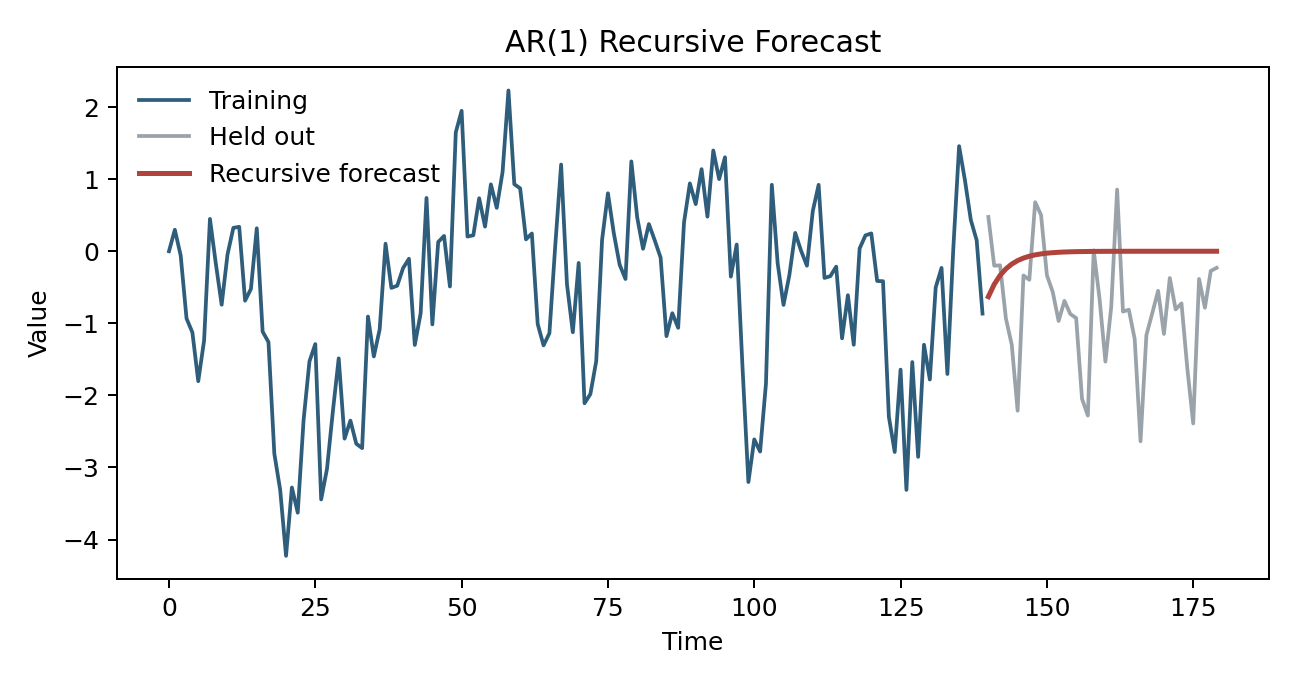
\includegraphics[width=0.86\textwidth]{ch07_fig01_ar_forecast.png}
  \caption{AR(1) 递归预测：多步预测逐渐回到长期均值。}
\end{figure}

\begin{figure}[htbp]
  \centering
  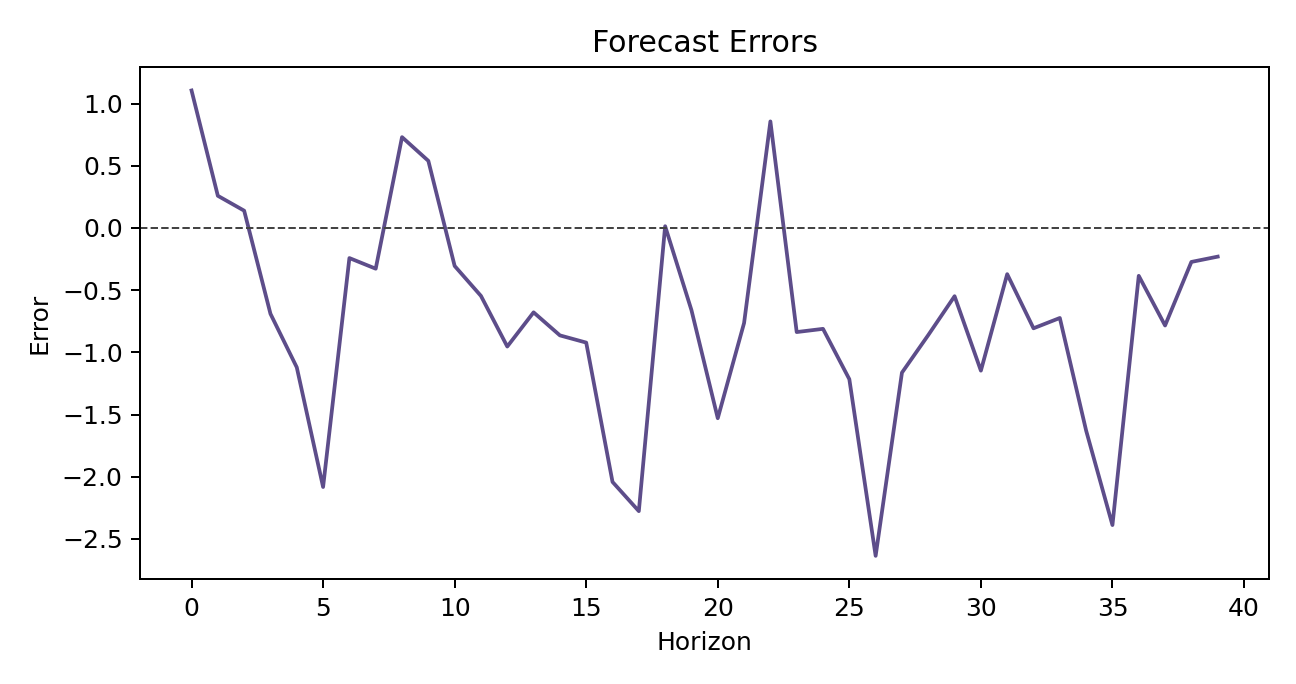
\includegraphics[width=0.86\textwidth]{ch07_fig02_forecast_errors.png}
  \caption{预测误差序列：用于检查预测是否存在系统性偏差或残余相关。}
\end{figure}

\section{练习提要}

原文练习主要围绕下列方向展开：
\begin{itemize}
  \item 用 AR(1) 和 AR(p) 公式计算一步、多步预测；
  \item 手算 Durbin-Levinson 递推的前几阶；
  \item 对太阳黑子或温度数据做预测并比较误差；
  \item 推导 ARCH/GARCH 条件方差预测。
\end{itemize}

\section*{本章小结}

第 7 章把投影理论落实为预测算法。AR 预测可递归计算，有限过去预测由 Durbin-Levinson 高效求解，ARMA 可放入 Kalman 滤波框架，非线性模型则常以条件方差预测为核心。

\clearpage
% Source: chapters/ch08_estimation_of_the_mean_and_covariance/第08章_Estimation_mean_covariance_均值与协方差估计.tex
\chapter{Estimation of the mean and covariance / 均值与协方差估计}
\section*{本章学习目标}

本章按照原文 \textit{Estimation of the mean and covariance} 的小节顺序整理，保留主要定义、定理、模型公式和练习方向，并将原文中的 R 实践思路改写为 Python 工程实践。

完成本章后，应能够：
\begin{itemize}
  \item 推导相关序列下样本均值的抽样性质；
  \item 定义样本自协方差和样本自相关；
  \item 理解自相关检验、Portmanteau 检验及稳健版本；
  \item 掌握 Newey-West/HAC 长期方差估计；
  \item 区分长记忆和均值结构变化。
\end{itemize}

\section{均值估计}

样本均值仍定义为
\[
  \bar X_n=\frac1n\sum_{t=1}^n X_t.
\]
若 \(\{X_t\}\) 为平稳线性过程且协方差绝对可和，则
\[
  \sqrt n(\bar X_n-\mu)\Rightarrow N(0,\sigma_L^2),
\qquad
  \sigma_L^2=\sum_{k=-\infty}^{\infty}c(k).
\]
\begin{theorem}[样本均值的渐近性质，原文 Theorem 8.1.1]
在线性时间序列和适当矩条件下，样本均值相合且渐近正态；渐近方差为长期方差，而不是单期方差 \(c(0)\)。
\end{theorem}

\section{协方差估计}

经验自协方差定义为
\[
  \hat c(h)=\frac1n\sum_{t=1}^{n-h}(X_t-\bar X)(X_{t+h}-\bar X),
\]
样本 ACF 为 \(\hat\rho(h)=\hat c(h)/\hat c(0)\)。

\begin{lemma}[经验协方差，原文 Lemma 8.2.1]
若均值已知或由样本均值替代，在平稳和矩条件下，\(\hat c(h)\) 是 \(c(h)\) 的相合估计。
\end{lemma}

\begin{theorem}[样本自协方差渐近分布，原文 Theorem 8.2.1--8.2.3]
对满足短记忆和四阶矩条件的线性序列，有限个样本自协方差组成的向量渐近正态，其协方差由二阶和四阶累积量决定。
\end{theorem}

\section{相关性检查}

白噪声检验常基于若干阶样本自相关。Box-Pierce/Ljung-Box 型统计量形如
\[
  Q_m=n\sum_{h=1}^m\hat\rho(h)^2
\]
或带有限样本修正。若序列为白噪声，\(Q_m\) 近似服从 \(\chi_m^2\)。

\subsection{稳健 Portmanteau 检验}

当存在条件异方差或更一般弱依赖时，普通 Portmanteau 检验的方差估计可能失真。稳健版本用 HAC 型协方差替代简单方差，以保持检验大小。

\section{偏相关检查}

样本 PACF 用于识别 AR 阶数。若真实模型为 AR(p)，则 p 阶之后的理论 PACF 为 0；样本 PACF 可用近似置信带判断是否显著。

\section{Newey-West 估计与拟合优度}

长期方差
\[
  \sigma_L^2=\sum_{k=-\infty}^{\infty}c(k)
\]
可用截断加权估计：
\[
  \hat\sigma_L^2=\hat c(0)+2\sum_{k=1}^{m}w_k\hat c(k),
\]
其中 Bartlett 权重为
\[
  w_k=1-\frac{k}{m+1}.
\]
这就是 Newey-West/HAC 估计的核心形式。

拟合优度检查通常对模型残差作 ACF、PACF 和 Portmanteau 检验。如果模型捕捉了线性依赖，残差应接近白噪声。

\section{长记忆与结构变化}

原文提醒：样本 ACF 缓慢衰减可能来自长记忆，也可能来自均值变化或趋势未处理。二者在图形上相似，但统计含义不同，需要结合趋势建模、分段分析和频域诊断判断。

\section{原文定理与练习补充}

\subsection{8.2.1 自协方差估计渐近性质}
\begin{theorem}[原文 Theorem 8.2.1]
若 \(\{X_t\}\) 为均值为 0 的线性平稳过程并满足矩条件，则固定滞后 \(h\) 的样本自协方差 \(\hat c(h)\) 相合，并具有渐近正态性质。
\end{theorem}

\subsection{8.2.2 样本自相关渐近性质}
\begin{theorem}[原文 Theorem 8.2.2--8.2.3]
样本自协方差和样本自相关组成的有限维向量在短记忆条件下渐近正态。该结果支撑 ACF 图置信带和相关性检验。
\end{theorem}

\subsection{8.2.3 样本自协方差之间的协方差}
\begin{example}[原文 Example 8.2.1]
对因果 AR(1) 模型 \(X_t=\phi X_{t-1}+\varepsilon_t\)，可显式计算样本自协方差极限协方差，用来说明不同滞后估计量之间并非独立。
\end{example}

\subsection{8.6 与 8.7}
第 8.6 节讨论模型拟合优度，第 8.7 节区分长记忆和均值变化。Exercise 8.1--8.3 研究 iid、MA(1) 和 block bootstrap；Exercise 8.4 检查偏相关。

\begin{lemma}[原文 Lemma 8.2.2]
在 Theorem 8.2.2 条件下，样本自相关可由样本自协方差通过 Delta 方法得到渐近分布。
\end{lemma}

\section{Python 工程实践}

在本章目录下运行：
\begin{lstlisting}[language=bash]
python scripts/ch08_generate_figures.py
\end{lstlisting}

脚本会把图像写入本章 \texttt{figures/} 目录。当前图像用于配合本章核心概念的仿真说明；若后续补齐原始数据文件，可把模拟数据替换为原文真实数据案例。

\begin{figure}[htbp]
  \centering
  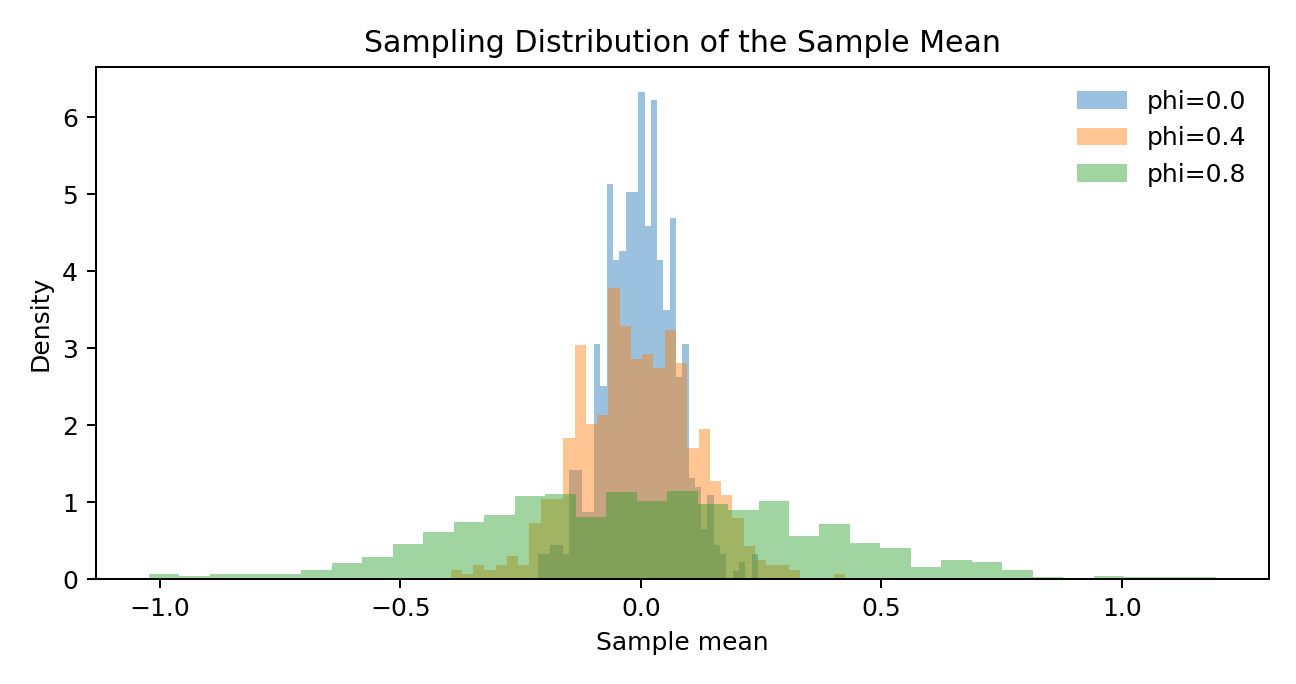
\includegraphics[width=0.86\textwidth]{ch08_fig01_sample_mean_dependence.png}
  \caption{不同相关强度下样本均值的抽样分布：相关性越强，有效样本量越小。}
\end{figure}

\begin{figure}[htbp]
  \centering
  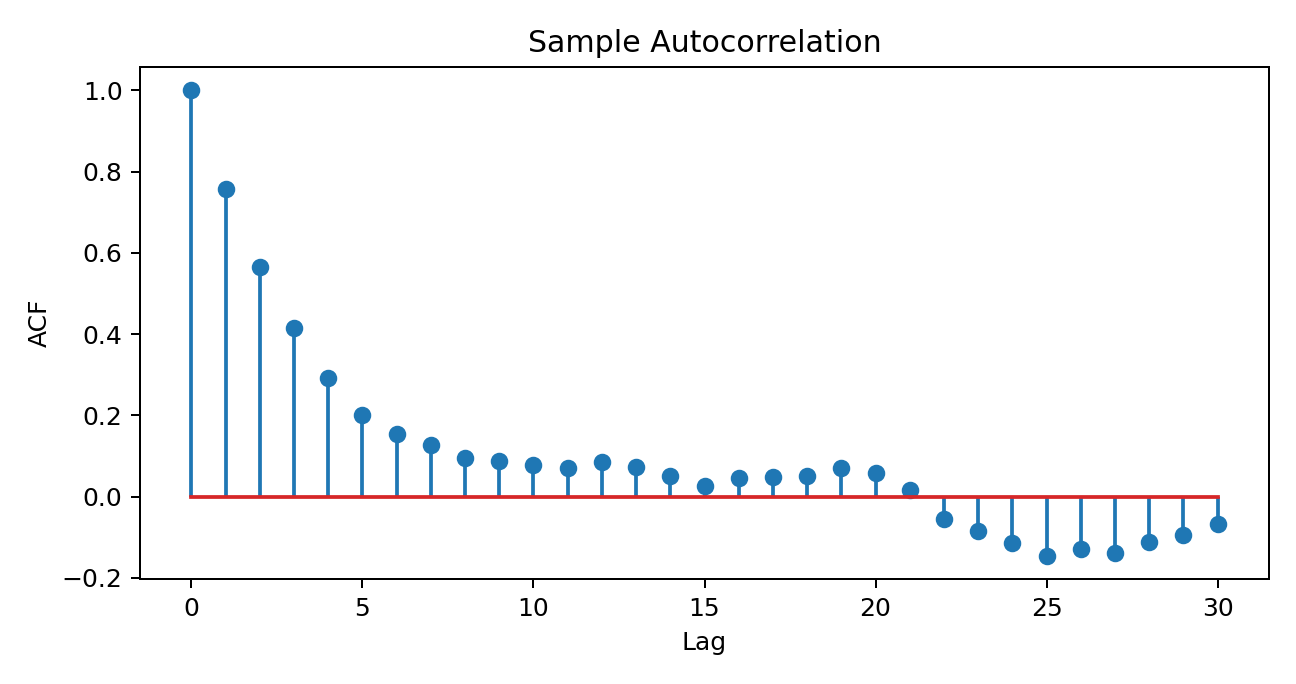
\includegraphics[width=0.86\textwidth]{ch08_fig02_sample_acf.png}
  \caption{样本 ACF 示例：估计序列在不同滞后上的线性依赖。}
\end{figure}

\section{练习提要}

原文练习主要围绕下列方向展开：
\begin{itemize}
  \item 在 iid、MA(1)、AR(1) 条件下推导样本自协方差的方差；
  \item 用 block bootstrap 估计样本均值的有限样本分布；
  \item 实现 Portmanteau 检验和稳健版本；
  \item 计算 Newey-West 标准误并比较普通标准误。
\end{itemize}

\section*{本章小结}

第 8 章把平稳理论转化为可计算估计量。均值、协方差、ACF、PACF 和长期方差估计是时间序列实证分析的基本工具，其中关键始终是正确处理相关性。

\clearpage
% Source: chapters/ch09_parameter_estimation/第09章_Parameter_estimation_参数估计.tex
\chapter{Parameter estimation / 参数估计}
\section*{本章学习目标}

本章按照原文 \textit{Parameter estimation} 的小节顺序整理，保留主要定义、定理、模型公式和练习方向，并将原文中的 R 实践思路改写为 Python 工程实践。

完成本章后，应能够：
\begin{itemize}
  \item 掌握 AR 模型的 Yule-Walker、条件最小二乘和高斯似然估计；
  \item 理解 Burg 算法与偏自相关递推；
  \item 描述 AR 估计量的抽样性质；
  \item 掌握 ARMA 的精确/近似高斯似然和 Kalman 滤波估计；
  \item 了解 Hannan-Rissanen 与 ARCH 准最大似然。
\end{itemize}

\section{自回归模型估计}

AR(p) 模型为
\[
  X_t=\phi_1X_{t-1}+\cdots+\phi_pX_{t-p}+\varepsilon_t.
\]
\subsection{Yule-Walker 估计}

理论方程为
\[
  \Gamma_p\phi=\gamma_p,
\]
其中 \(\Gamma_p=(c(i-j))_{i,j=1}^p\)，\(\gamma_p=(c(1),\ldots,c(p))'\)。用样本自协方差替代即可得
\[
  \hat\phi_{YW}=\hat\Gamma_p^{-1}\hat\gamma_p.
\]

\subsection{高斯似然}

若 \(X=(X_1,\ldots,X_n)'\sim N(0,\Sigma_\theta)\)，高斯负对数似然差一个常数为
\[
  \ell(\theta)=\log|\Sigma_\theta|+X'\Sigma_\theta^{-1}X.
\]
该形式精确但计算协方差矩阵和逆矩阵成本较高。

\section{条件高斯似然与最小二乘}

条件在初始 \(X_1,\ldots,X_p\) 上，AR(p) 的条件残差为
\[
  e_t(\phi)=X_t-\phi_1X_{t-1}-\cdots-\phi_pX_{t-p}.
\]
条件最小二乘估计为
\[
  \hat\phi_{CLS}
  =\arg\min_\phi\sum_{t=p+1}^n e_t(\phi)^2.
\]
它把 AR 估计转化为普通回归问题。

\subsection{Burg 算法}

Burg 算法通过同时最小化前向和后向预测误差估计反射系数，保证估计得到的 AR 模型稳定。其递推与 Levinson-Durbin 和 PACF 紧密相关。

\section{AR 估计量的抽样性质}

\begin{definition}[鞅差，原文 Definition 9.1.1]
若 \(E(Z_t\mid\mathcal F_{t-1})=0\)，则称 \(\{Z_t\}\) 为鞅差序列。
\end{definition}

在稳定 AR 模型和适当矩条件下，Yule-Walker、条件最小二乘和高斯似然估计量通常相合且渐近正态：
\[
  \sqrt n(\hat\phi-\phi_0)\Rightarrow N(0,V).
\]
证明核心是把估计方程展开为鞅差和可忽略项。

\section{ARMA 模型估计}

ARMA(p,q)
\[
  \phi(B)X_t=\theta(B)\varepsilon_t
\]
的似然需要根据参数递归计算创新。常见方法包括精确高斯最大似然、近似高斯似然和 Kalman 滤波。

\begin{theorem}[ARMA GMLE 抽样性质，原文 Theorem 9.2.1]
在因果、可逆、可识别和矩条件下，ARMA 高斯最大似然估计量相合并渐近正态。
\end{theorem}

\subsection{Hannan-Rissanen 方法}

该方法先用高阶 AR 近似 ARMA 的 \(AR(\infty)\) 表示，估计创新，再用回归估计 ARMA 参数，是一种计算上较快的初值或估计方案。

\section{ARCH 准最大似然}

ARCH/GARCH 中即使创新非高斯，也常使用高斯准似然。只要条件均值和条件方差设定正确，参数仍可具有良好渐近性质。

\section{原文定理、例题与算法补充}

\subsection{Yule-Walker 技术引理}
\begin{lemma}[原文 Lemma 9.1.1]
对零均值随机向量 \(Z\)，二次型和协方差矩阵的性质可用于控制 Yule-Walker 估计误差。这一引理服务于 AR 参数估计量的抽样性质。
\end{lemma}

\subsection{AR(1) 高斯似然例题}
\begin{example}[原文 Example 9.1.1]
在 AR(1) 情形，协方差矩阵和条件分布都可显式写出，因此能直接看出精确高斯似然与条件似然之间的差别。
\end{example}

\subsection{Yule-Walker 与最小二乘玩具例子}
\begin{example}[原文 Example 9.1.2]
原文用一个小例子比较 Yule-Walker 与最小二乘。二者都估计 AR 参数，但一个从样本协方差方程出发，另一个从预测残差平方和出发。
\end{example}

\subsection{AR 估计量渐近理论}
\begin{theorem}[原文 Theorem 9.1.1]
在鞅差和矩条件下，AR 估计方程的主项满足中心极限定理，从而得到参数估计量的渐近正态性。
\end{theorem}

\subsection{ARMA 最大似然与 Hannan-Rissanen}
\begin{theorem}[原文 Theorem 9.2.1]
若 ARMA 模型因果、可逆、可识别且满足矩条件，高斯最大似然估计量相合并渐近正态。
\end{theorem}

Exercise 9.1 要求用普通最小二乘估计 AR 参数并与软件输出比较；Exercise 9.2 研究随机自回归模型的参数估计。Burg 算法、Kalman 似然和 Hannan-Rissanen 方法共同构成 ARMA 估计的实用工具箱。

\section{Python 工程实践}

在本章目录下运行：
\begin{lstlisting}[language=bash]
python scripts/ch09_generate_figures.py
\end{lstlisting}

脚本会把图像写入本章 \texttt{figures/} 目录。当前图像用于配合本章核心概念的仿真说明；若后续补齐原始数据文件，可把模拟数据替换为原文真实数据案例。

\begin{figure}[htbp]
  \centering
  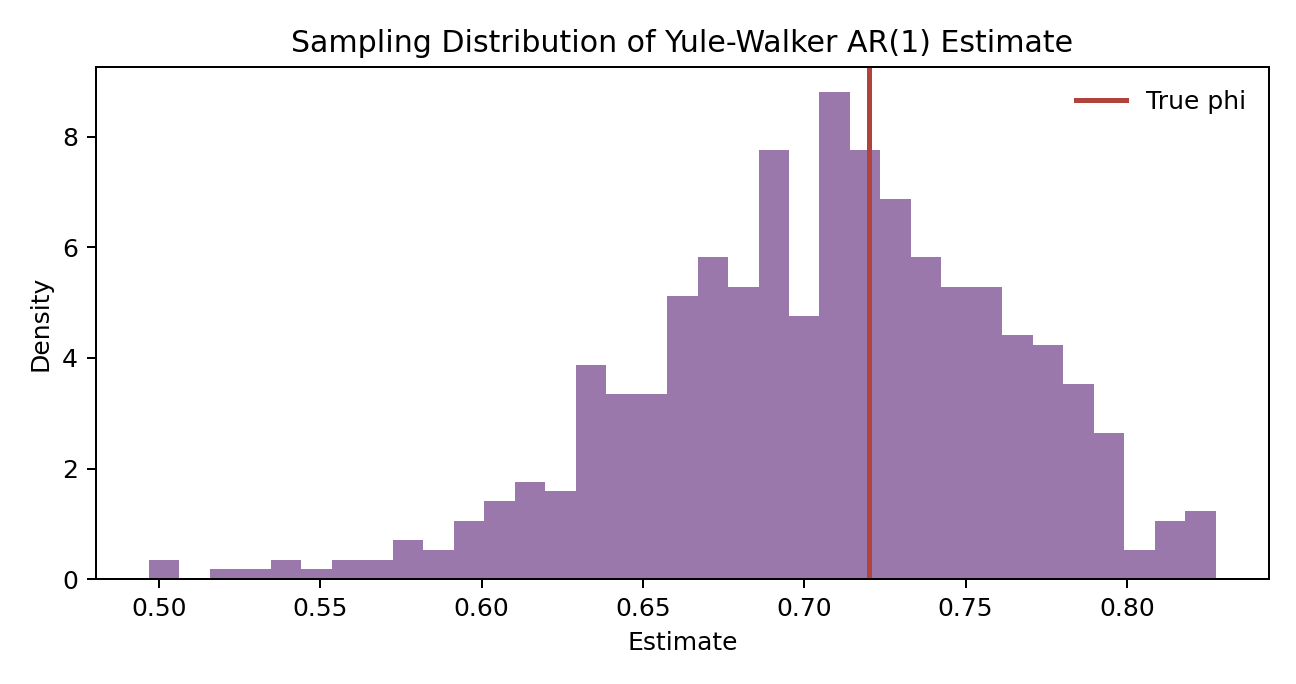
\includegraphics[width=0.86\textwidth]{ch09_fig01_yule_walker_sampling.png}
  \caption{Yule-Walker AR(1) 估计量的抽样分布：样本量有限时估计量围绕真值波动。}
\end{figure}

\begin{figure}[htbp]
  \centering
  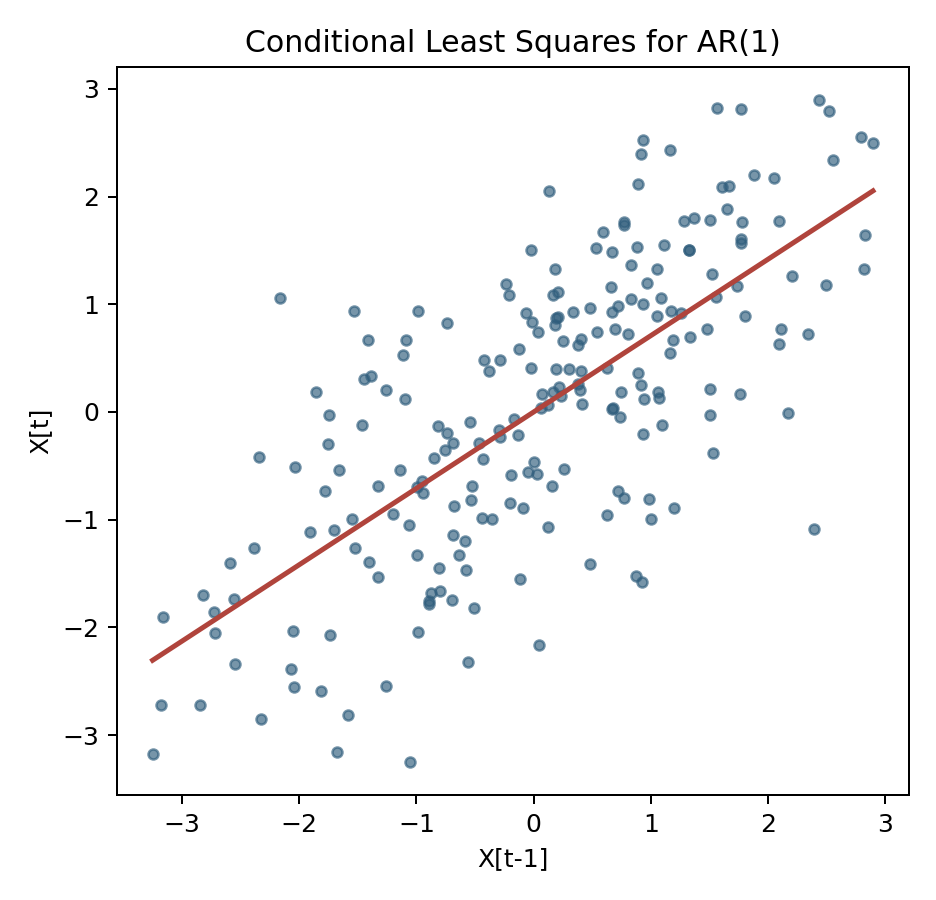
\includegraphics[width=0.86\textwidth]{ch09_fig02_cls_ar1.png}
  \caption{AR(1) 条件最小二乘：把 \(X_t\) 对 \(X_{t-1}\) 做回归得到参数估计。}
\end{figure}

\section{练习提要}

原文练习主要围绕下列方向展开：
\begin{itemize}
  \item 用 OLS、Yule-Walker 和 MLE 估计同一 AR 模型并比较；
  \item 推导 AR(1) 高斯似然的简单形式；
  \item 实现 Burg 算法或调用库函数比较结果；
  \item 估计随机系数 AR 或 ARCH 模型。
\end{itemize}

\section*{本章小结}

第 9 章集中讨论模型参数如何从数据中估计。AR 模型可由协方差方程、回归或似然估计；ARMA 估计更依赖创新递推和数值优化；渐近理论则解释估计误差如何随样本量缩小。

\clearpage
% Source: chapters/ch10_spectral_representations/第10章_Spectral_Representations_谱表示.tex
\chapter{Spectral Representations / 谱表示}
\section*{本章学习目标}

本章按照原文 \textit{Spectral Representations} 的小节顺序整理，保留主要定义、定理、模型公式和练习方向，并将原文中的 R 实践思路改写为 Python 工程实践。

完成本章后，应能够：
\begin{itemize}
  \item 回顾 DFT 在周期检测中的作用；
  \item 理解平稳序列 DFT 的近似不相关性；
  \item 掌握谱密度、谱分布和 Bochner/Herglotz 定理；
  \item 理解 Cramer 谱表示定理；
  \item 推导 MA、AR、ARMA 的谱密度。
\end{itemize}

\section{Fourier 变换的使用回顾}

前面章节已经用 DFT 找周期。对 \(X_1,\ldots,X_n\)，DFT 为
\[
  J_n(\omega)=\frac1{\sqrt n}\sum_{t=1}^n X_t e^{it\omega},
\]
周期图为 \(I_n(\omega)=|J_n(\omega)|^2\)。本章把频域工具从周期检测推广到平稳过程的完整二阶表示。

\section{DFT 的近似不相关性}

\begin{lemma}[原文 Lemma 10.2.1]
若 \(\{X_t\}\) 二阶平稳且自协方差绝对可和，则不同 Fourier 频率处的 DFT 近似不相关：
\[
  \mathrm{cov}\{J_n(\omega_j),J_n(\omega_k)\}\approx0,\qquad j\ne k.
\]
同一频率处的方差近似为谱密度。
\end{lemma}

该性质解释了为什么频域似然和 Whittle 似然可把复杂相关矩阵近似分解为频率上的独立贡献。

\section{谱表示结果概览}

频域分析的中心思想是：平稳序列的协方差函数和频率能量分布互为 Fourier 对。

\subsection{谱密度}

若 \(\sum_k|c(k)|<\infty\)，谱密度定义为
\[
  f(\omega)=\frac1{2\pi}\sum_{k=-\infty}^{\infty}c(k)e^{-ik\omega}.
\]
反演公式为
\[
  c(k)=\int_{-\pi}^{\pi}e^{ik\omega}f(\omega)\,d\omega.
\]

\begin{theorem}[谱密度非负性，原文 Theorem 10.4.1]
合法协方差序列的谱密度非负；反过来，非负可积函数通过反演公式定义合法协方差。
\end{theorem}

\section{谱分布与 Bochner 定理}

若协方差不绝对可和，也可用谱分布 \(F\) 表示：
\[
  c(k)=\int_{-\pi}^{\pi}e^{ik\omega}\,dF(\omega).
\]
\begin{theorem}[Herglotz/Bochner 定理，原文 Theorem 10.4.2]
序列 \(c(k)\) 非负定，当且仅当存在有限非负测度 \(F\)，使上述表示成立。
\end{theorem}

\section{谱表示定理}

\begin{theorem}[Cramer 谱表示，原文 Theorem 10.5.1]
零均值二阶平稳过程可写成
\[
  X_t=\int_{-\pi}^{\pi}e^{it\omega}\,dZ(\omega),
\]
其中 \(Z(\omega)\) 是正交增量过程，且增量方差由谱分布决定。
\end{theorem}

这一定理是 Wold 分解在频域中的对应物。

\section{MA、AR 和 ARMA 的谱密度}

线性过程
\[
  X_t=\sum_{j=0}^{\infty}\psi_j\varepsilon_{t-j}
\]
的谱密度为
\[
  f_X(\omega)=\frac{\sigma^2}{2\pi}
  \left|\sum_{j=0}^{\infty}\psi_je^{-ij\omega}\right|^2.
\]
ARMA(p,q) 的谱密度为
\[
  f_X(\omega)=\frac{\sigma^2}{2\pi}
  \frac{|\theta(e^{-i\omega})|^2}{|\phi(e^{-i\omega})|^2}.
\]
AR 根接近单位圆会在相应频率附近产生高谱峰。

\section{高阶谱与扩展}

原文还介绍累积量和高阶谱。二阶谱描述协方差结构，高阶谱则可捕捉非高斯和非线性依赖。缺失观测情形下，谱密度估计还需修正采样机制带来的影响。

\section{原文小节覆盖补充}

\subsection{DFT 近似不相关与平稳性检验}
第 10.2 节证明二阶平稳短记忆序列在不同 Fourier 频率上的 DFT 近似不相关。第 10.2.1 用该性质讨论二阶平稳性检验：若局部频域能量随时间变化，平稳性可能失效。Exercise 10.1 要求模拟 AR(2) 并运行相应检验。

\begin{lemma}[DFT 协方差，原文 Lemma 10.2.1--10.2.2]
若自协方差及其加权和满足可和条件，则 DFT 协方差由谱密度近似，不同 Fourier 频率之间的协方差趋于 0。
\end{lemma}

\subsection{完整去相关与谱表示总览}
第 10.2.3 解释 DFT 在理想情形下的完全去相关。第 10.3 总结 Cramer 谱表示和 Bochner/Herglotz 定理：前者表示过程本身，后者表示协方差函数。

\subsection{谱密度、谱分布和例子}
第 10.4 讨论谱密度非负性、经验协方差的谱解释、Toeplitz 方差矩阵和谱分布。纯周期成分对应谱分布跳跃，随机平稳成分对应连续谱密度。

\begin{example}[谱分布例子，原文 Example 10.4.2--10.4.3]
确定性正弦波的谱分布在对应频率处有质量点；一般平稳随机过程则通过连续谱密度分配频率能量。
\end{example}

\subsection{线性过程和 ARMA 谱密度}
第 10.6 从线性过程推出
\[
  f_X(\omega)=\frac{\sigma^2}{2\pi}|\psi(e^{-i\omega})|^2,
\]
并得到 ARMA 谱密度。Exercise 10.2 要求推导 MA(1) 谱密度。

\begin{definition}[Cramer 表示，原文 Definition 10.6.1]
线性过程可写为正交增量过程的频域积分，使滤波、谱密度和协方差反演处在统一框架内。
\end{definition}

\subsection{谱密度近似、高阶谱和附录证明}
第 10.6.3 讨论用 AR 或 MA 近似谱密度。第 10.7 引入高阶谱，第 10.8 讨论随机缺失，第 10.9 给出一般正交展开等证明。

\begin{proposition}[高阶谱，原文 Proposition 10.7.1]
若严格平稳序列具有足够高阶累积量可和性，则 q 阶谱密度定义为 q 阶累积量函数的 Fourier 变换。
\end{proposition}

\subsection{谱密度近似引理}
\begin{lemma}[原文 Lemma 10.6.1]
若 \(|c(r)|\) 可和，截断协方差对应的谱密度近似真实谱密度，误差由截断尾部控制。
\end{lemma}

\begin{lemma}[原文 Lemma 10.6.2]
若谱密度足够平滑，可用有限阶 AR 或 MA 近似其形状；该思想连接谱估计和高阶 AR 近似。
\end{lemma}

\begin{theorem}[原文 Theorem 10.9.1]
一般正交展开定理说明，不一定平稳的时间序列也可在适当正交基下展开；Cramer 表示是平稳情形的特殊版本。
\end{theorem}

\subsection{10.9 附录证明的教学作用}
原文附录的证明把谱密度非负性、谱分布构造、正交增量和一般正交展开连在一起。教学上应把它理解为三步：先由非负定协方差构造非负谱测度；再用该测度定义频域正交增量；最后用积分表示恢复时域过程。这样，Bochner 定理、Cramer 表示和 ARMA 谱密度公式就不再是孤立结论，而是同一套 Hilbert 空间投影思想在频域中的表现。

\section{Python 工程实践}

在本章目录下运行：
\begin{lstlisting}[language=bash]
python scripts/ch10_generate_figures.py
\end{lstlisting}

脚本会把图像写入本章 \texttt{figures/} 目录。当前图像用于配合本章核心概念的仿真说明；若后续补齐原始数据文件，可把模拟数据替换为原文真实数据案例。

\begin{figure}[htbp]
  \centering
  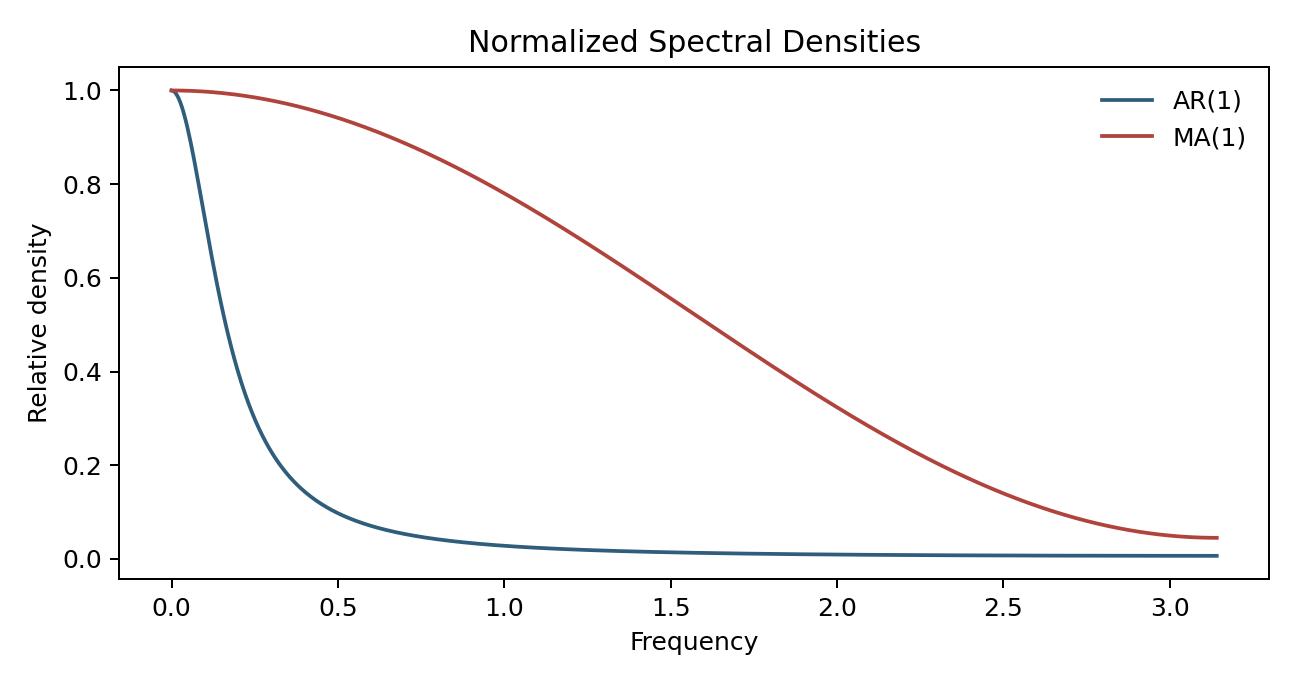
\includegraphics[width=0.86\textwidth]{ch10_fig01_spectral_density.png}
  \caption{AR 与 MA 谱密度形态：频域中不同模型表现为不同频率能量分布。}
\end{figure}

\begin{figure}[htbp]
  \centering
  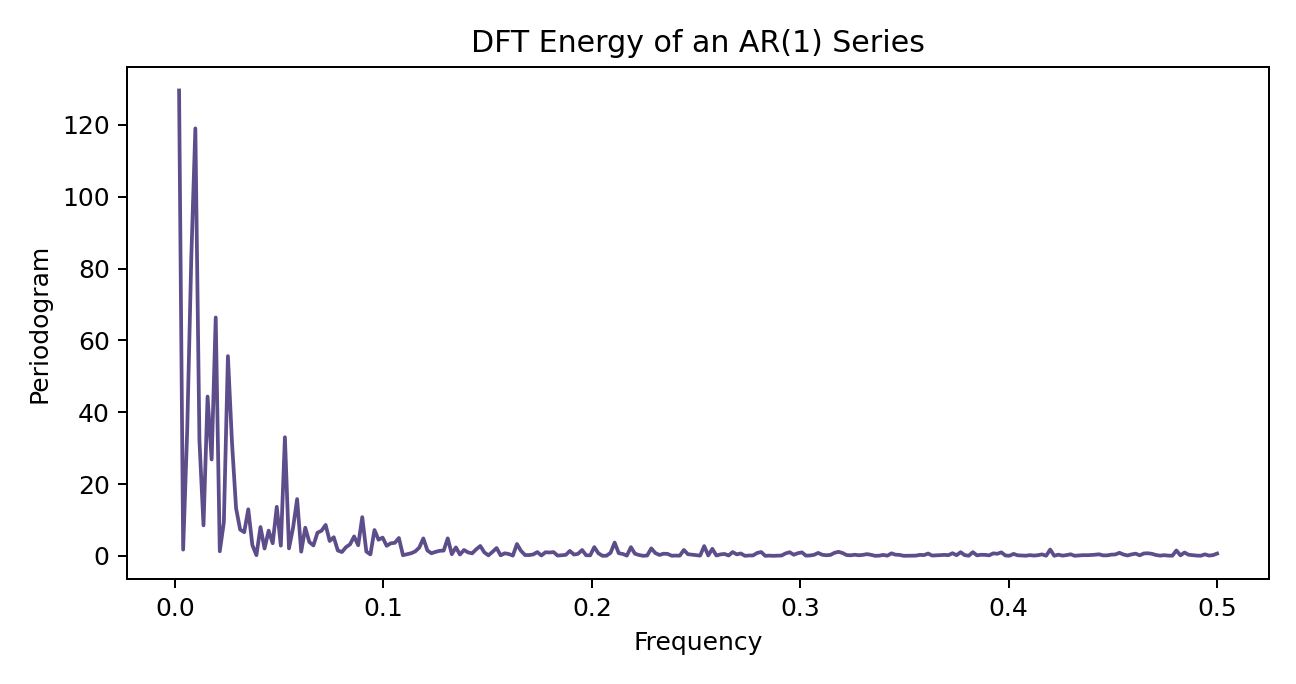
\includegraphics[width=0.86\textwidth]{ch10_fig02_dft_energy.png}
  \caption{AR(1) 序列的 DFT 能量：低频能量较强对应高持续性。}
\end{figure}

\section{练习提要}

原文练习主要围绕下列方向展开：
\begin{itemize}
  \item 推导 MA(1)、AR(1) 和 ARMA(p,q) 谱密度；
  \item 模拟 AR(2)，观察 DFT 和周期图峰值；
  \item 验证协方差和谱密度的 Fourier 反演；
  \item 阅读高阶谱定义并联系非高斯过程。
\end{itemize}

\section*{本章小结}

第 10 章给出了平稳过程的频域语言。协方差函数、谱密度和谱分布互相等价，DFT 近似去相关使频域估计成为可能，ARMA 谱密度则把模型根的位置转化为频率峰值。

\clearpage
% Source: chapters/ch11_spectral_analysis/第11章_Spectral_Analysis_谱分析.tex
\chapter{Spectral Analysis / 谱分析}
\section*{本章学习目标}

本章按照原文 \textit{Spectral Analysis} 的小节顺序整理，保留主要定义、定理、模型公式和练习方向，并将原文中的 R 实践思路改写为 Python 工程实践。

完成本章后，应能够：
\begin{itemize}
  \item 理解 DFT 和周期图的抽样分布；
  \item 掌握谱密度估计的滞后窗和平滑周期图方法；
  \item 理解 Whittle 似然及其与高斯似然的关系；
  \item 了解比率统计在时间序列中的作用；
  \item 进行线性模型拟合优度检验。
\end{itemize}

\section{DFT 与周期图}

周期图定义为
\[
  I_n(\omega)=\frac1n\left|\sum_{t=1}^n X_t e^{it\omega}\right|^2.
\]
\begin{lemma}[原文 Lemma 11.1.1]
在零均值二阶平稳和短记忆条件下，DFT 的二阶矩由谱密度近似控制，不同 Fourier 频率近似不相关。
\end{lemma}

周期图是谱密度的原始估计，但它本身不相合：样本量增大时方差并不自动消失。

\section{DFT 和周期图的分布}

对线性过程，在适当系数可和和矩条件下，
\[
  J_n(\omega_j)\approx \mathcal{CN}(0,2\pi f(\omega_j)),
\]
因此
\[
  \frac{I_n(\omega_j)}{2\pi f(\omega_j)}
\]
近似服从指数分布。原文用一系列引理和定理证明这一近似，并说明不同频率近似独立。

\section{谱密度估计}

\subsection{滞后窗估计}

用样本自协方差和窗口 \(w(\cdot)\) 可定义
\[
  \hat f(\omega)=\frac1{2\pi}\sum_{|k|\le m}w(k/m)\hat c(k)e^{-ik\omega}.
\]
窗口截断降低方差，但会引入偏差。

\subsection{平滑周期图}

另一种等价做法是在频域中平均邻近周期图：
\[
  \hat f(\omega)=\sum_j W_m(\omega-\omega_j)I_n(\omega_j).
\]
\begin{theorem}[谱估计抽样性质，原文 Theorem 11.3.1]
在平稳、短记忆和带宽条件下，平滑谱估计渐近无偏且方差随带宽增加而下降。
\end{theorem}

\section{Whittle 似然与比率统计}

Whittle 似然把 DFT 近似独立性用于参数估计：
\[
  L_W(\theta)=\sum_{\omega_j}
  \left\{\log f_\theta(\omega_j)+\frac{I_n(\omega_j)}{f_\theta(\omega_j)}\right\}.
\]
它近似高斯似然，但避免直接处理大型 Toeplitz 协方差矩阵。

\subsection{比率统计}

若把周期图与拟合谱密度作比
\[
  R(\omega_j)=\frac{I_n(\omega_j)}{f_{\hat\theta}(\omega_j)},
\]
模型拟合良好时，比率应近似白噪声频域形态。原文进一步讨论了基于比率的检验统计量。

\section{拟合优度检验}

线性时间序列模型拟合后，应检查残差和标准化周期图是否仍含系统性频率结构。谱域拟合优度检验与第 8 章的 ACF/Portmanteau 检验互为补充。

\section{原文小节覆盖补充}

\subsection{周期图分布的线性过程条件}
若 \(X_t=\sum_{j=0}^{\infty}\psi_j\varepsilon_{t-j}\) 且 \(\sum j^{1/2}|\psi_j|<\infty\)，则 DFT 渐近复正态，标准化周期图近似指数分布。

\begin{lemma}[线性过程 DFT，原文 Lemma 11.2.1--11.2.2]
线性过程的 DFT 可写为创新 DFT 乘以传递函数再加边界误差；在系数可和条件下边界误差可忽略。
\end{lemma}

\begin{proposition}[创新 DFT，原文 Proposition 11.2.1]
iid 创新的 DFT 在不同 Fourier 频率上渐近独立复正态，是一般线性过程结果的基础。
\end{proposition}

\begin{theorem}[周期图渐近分布，原文 Theorem 11.2.1]
在线性过程和矩条件下，不同 Fourier 频率处的周期图近似独立，且 \(I_n(\omega_j)/f(\omega_j)\) 近似指数型分布。
\end{theorem}

\subsection{滞后窗与谱窗例子}
Example 11.3.1 展示常见 lag windows。Example 11.3.2 展示 spectral windows。滞后窗估计在时域截断协方差，谱窗估计在频域平滑周期图。

\begin{lemma}[滞后窗期望，原文 Lemma 11.3.1]
谱估计的期望等于真实谱密度与谱窗的卷积，因此窗口宽度控制偏差和平滑程度。
\end{lemma}

\begin{lemma}[谱窗正则性，原文 Lemma 11.3.2]
若核函数有有界导数，则离散谱窗可稳定近似连续卷积，为渐近性质提供技术条件。
\end{lemma}

\subsection{Whittle 似然性质}
Example 11.4.1 给出 ARMA(1,1) 拟合。Whittle 似然衡量模型谱密度与周期图的匹配，避免直接处理大型 Toeplitz 协方差矩阵。

\begin{lemma}[Whittle 展开，原文 Lemma 11.4.1--11.4.3]
在因果 ARMA 和平滑条件下，Whittle 目标函数一致收敛，其导数展开可用于证明估计量一致和渐近正态。
\end{lemma}

\begin{theorem}[Whittle 渐近性质，原文 Theorem 11.4.1]
若模型正确且满足正则条件，Whittle 估计量渐近正态，极限方差由谱密度对参数的导数决定。
\end{theorem}

\subsection{比率统计和拟合优度}
第 11.5 节研究标准化周期图的比率统计。若模型拟合好，\(I_n(\omega)/f_{\hat\theta}(\omega)\) 不应呈现系统频率结构。Example 11.5.1 用 Whittle 似然说明该形式。第 11.6 节据此构造线性时间序列模型拟合优度检验，附录第 11.7 节给出技术引理。

\section{Python 工程实践}

在本章目录下运行：
\begin{lstlisting}[language=bash]
python scripts/ch11_generate_figures.py
\end{lstlisting}

脚本会把图像写入本章 \texttt{figures/} 目录。当前图像用于配合本章核心概念的仿真说明；若后续补齐原始数据文件，可把模拟数据替换为原文真实数据案例。

\begin{figure}[htbp]
  \centering
  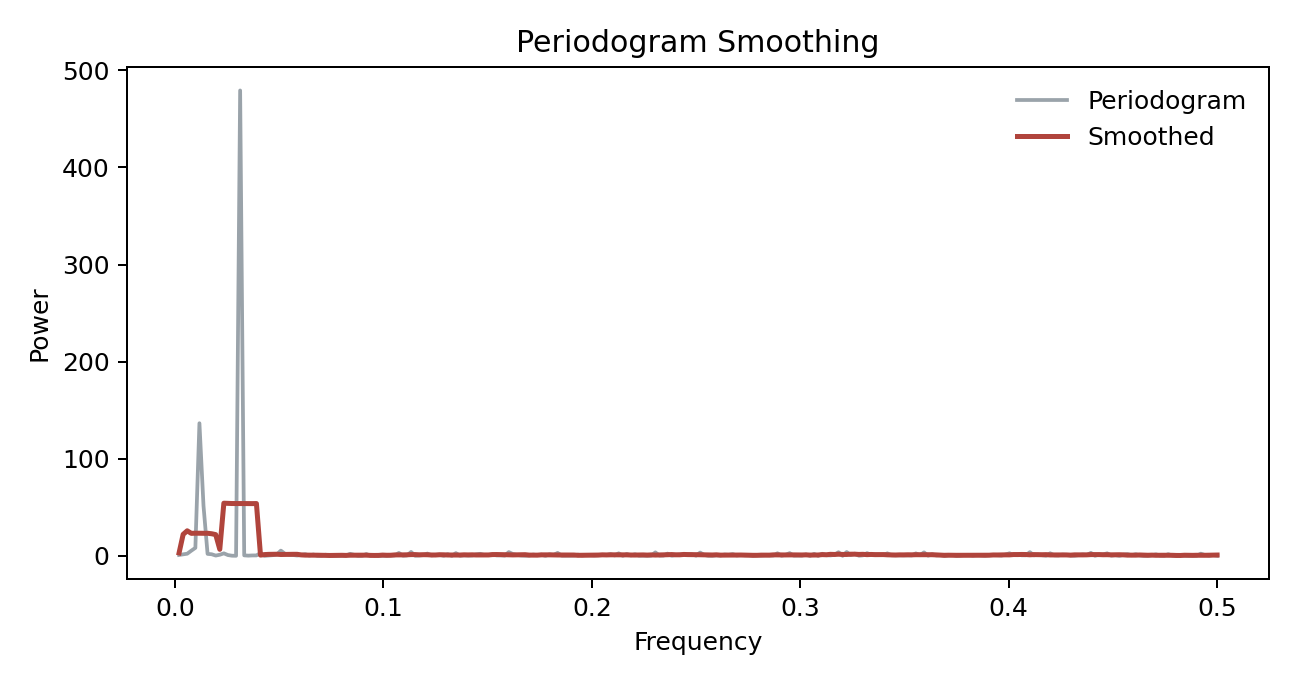
\includegraphics[width=0.86\textwidth]{ch11_fig01_smoothed_periodogram.png}
  \caption{周期图平滑：原始周期图方差大，平滑后更接近谱密度形状。}
\end{figure}

\begin{figure}[htbp]
  \centering
  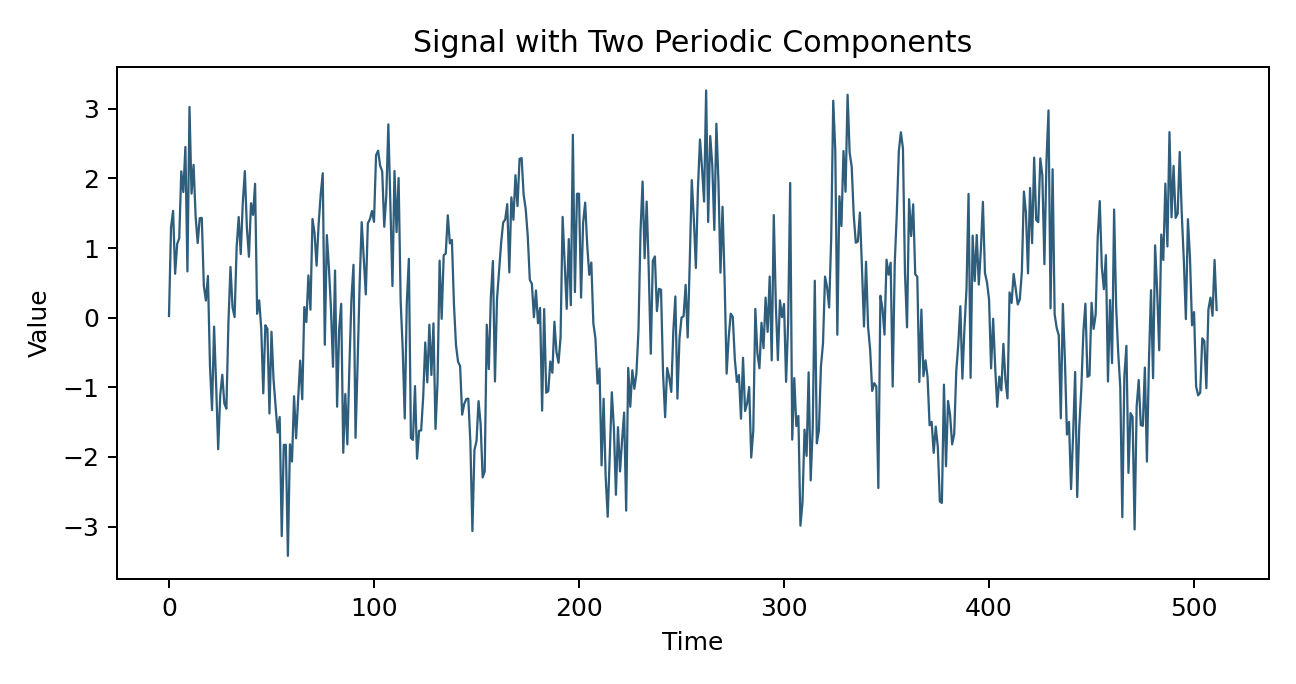
\includegraphics[width=0.86\textwidth]{ch11_fig02_two_frequency_signal.png}
  \caption{双频信号：时域叠加的周期成分会在频域形成多个峰。}
\end{figure}

\section{练习提要}

原文练习主要围绕下列方向展开：
\begin{itemize}
  \item 模拟线性过程并比较周期图与理论谱密度；
  \item 实现 Bartlett、Daniell 等平滑窗口；
  \item 用 Whittle 似然拟合 ARMA 模型；
  \item 基于标准化周期图检查模型拟合优度。
\end{itemize}

\section*{本章小结}

第 11 章从谱表示走向谱估计。周期图是入口但不相合，平滑和窗口提供稳定估计；Whittle 似然利用频域近似独立性，给出高效的参数估计和拟合检验工具。

\clearpage
% Source: chapters/ch12_multivariate_time_series/第12章_Multivariate_time_series_多元时间序列.tex
\chapter{Multivariate time series / 多元时间序列}
\section*{本章学习目标}

本章按照原文 \textit{Multivariate time series} 的小节顺序整理，保留主要定义、定理、模型公式和练习方向，并将原文中的 R 实践思路改写为 Python 工程实践。

完成本章后，应能够：
\begin{itemize}
  \item 复习序列卷积和矩阵谱表示；
  \item 建立多元时间序列回归模型；
  \item 理解条件独立、偏相关和相干性；
  \item 定义交叉谱密度和谱偏相关；
  \item 解释逆谱密度矩阵的条件依赖含义。
\end{itemize}

\section{背景}

\subsection{序列与卷积}

若 \(a=\{a_j\}\)、\(b=\{b_j\}\)，卷积定义为
\[
  (a*b)_k=\sum_j a_jb_{k-j}.
\]
多元线性滤波中，系数可为矩阵，卷积描述不同序列和不同滞后之间的相互作用。

\subsection{谱表示}

多元平稳序列 \(X_t\in\mathbb R^d\) 的自协方差矩阵为
\[
  \Gamma(h)=E(X_{t+h}X_t').
\]
谱密度矩阵定义为
\[
  f(\omega)=\frac1{2\pi}\sum_{h=-\infty}^{\infty}\Gamma(h)e^{-ih\omega}.
\]
它在每个频率上是 Hermitian 非负定矩阵。

\section{多元时间序列回归}

多元线性模型可写为
\[
  Y_t=\sum_{j}A_jX_{t-j}+\varepsilon_t.
\]
向量自回归 VAR(p) 是典型例子：
\[
  X_t=A_1X_{t-1}+\cdots+A_pX_{t-p}+\varepsilon_t.
\]
矩阵 \(A_j\) 描述一个变量过去值对另一个变量当前值的动态影响。

\subsection{条件独立}

若一个分量在给定其他序列后不能由另一分量改善预测，则称二者条件线性不相关。高斯情形下，这可进一步解释为条件独立。

\section{偏相关、相干性与交叉谱}

两个序列的交叉谱密度 \(f_{12}(\omega)\) 是交叉协方差的 Fourier 变换。相干性定义为
\[
  \mathrm{coh}_{12}(\omega)
  =\frac{|f_{12}(\omega)|^2}{f_{11}(\omega)f_{22}(\omega)}.
\]
它是频域中的相关系数平方，取值在 \([0,1]\)。

谱偏相关是在给定其他序列后定义的频域相关，类似多元分析中的偏相关。

\section{逆谱密度矩阵}

设
\[
  g(\omega)=f(\omega)^{-1}.
\]
逆谱密度矩阵的零元素表示频域条件不相关结构。对高斯平稳序列，若 \(g_{ij}(\omega)=0\) 对所有 \(\omega\) 成立，则第 \(i\) 和第 \(j\) 个序列在给定其他序列后条件独立。

原文还证明了公式 (12.6)，把谱偏相关和逆谱密度矩阵联系起来。这一结构是高维多元时间序列图模型的基础。

\section{Python 工程实践}

在本章目录下运行：
\begin{lstlisting}[language=bash]
python scripts/ch12_generate_figures.py
\end{lstlisting}

脚本会把图像写入本章 \texttt{figures/} 目录。当前图像用于配合本章核心概念的仿真说明；若后续补齐原始数据文件，可把模拟数据替换为原文真实数据案例。

\begin{figure}[htbp]
  \centering
  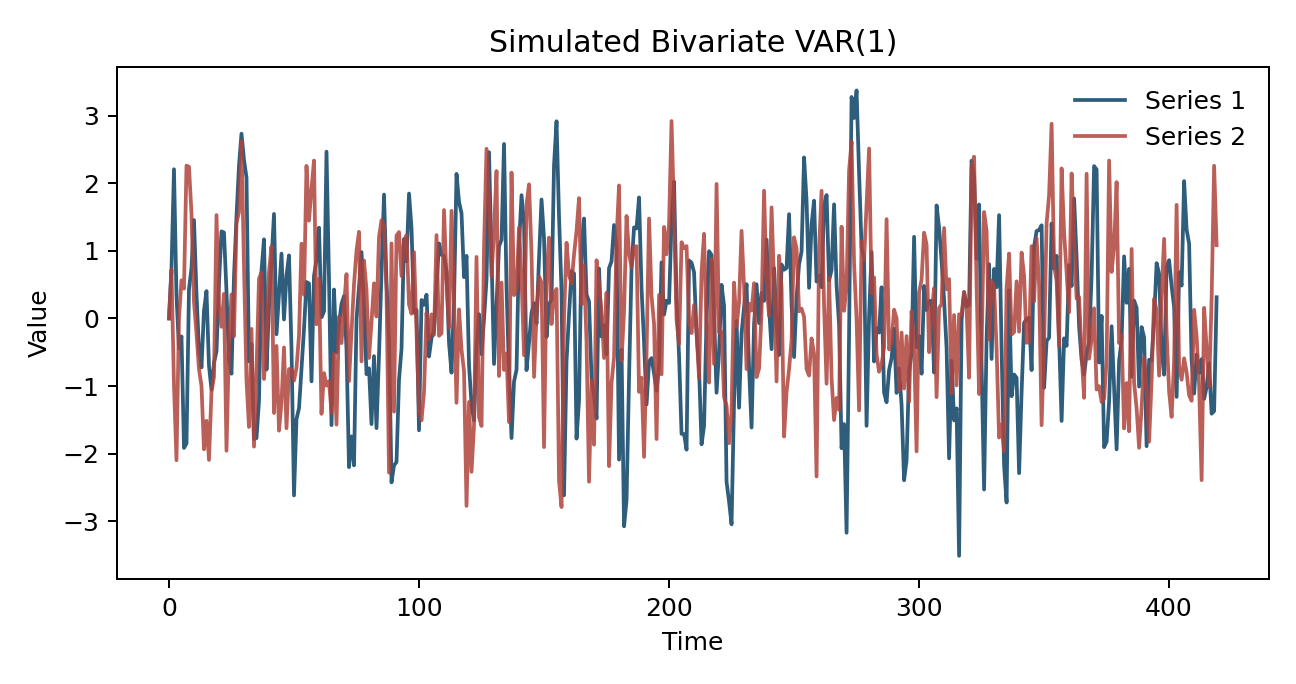
\includegraphics[width=0.86\textwidth]{ch12_fig01_var_series.png}
  \caption{二元 VAR(1) 模拟序列：两个变量通过滞后矩阵相互影响。}
\end{figure}

\begin{figure}[htbp]
  \centering
  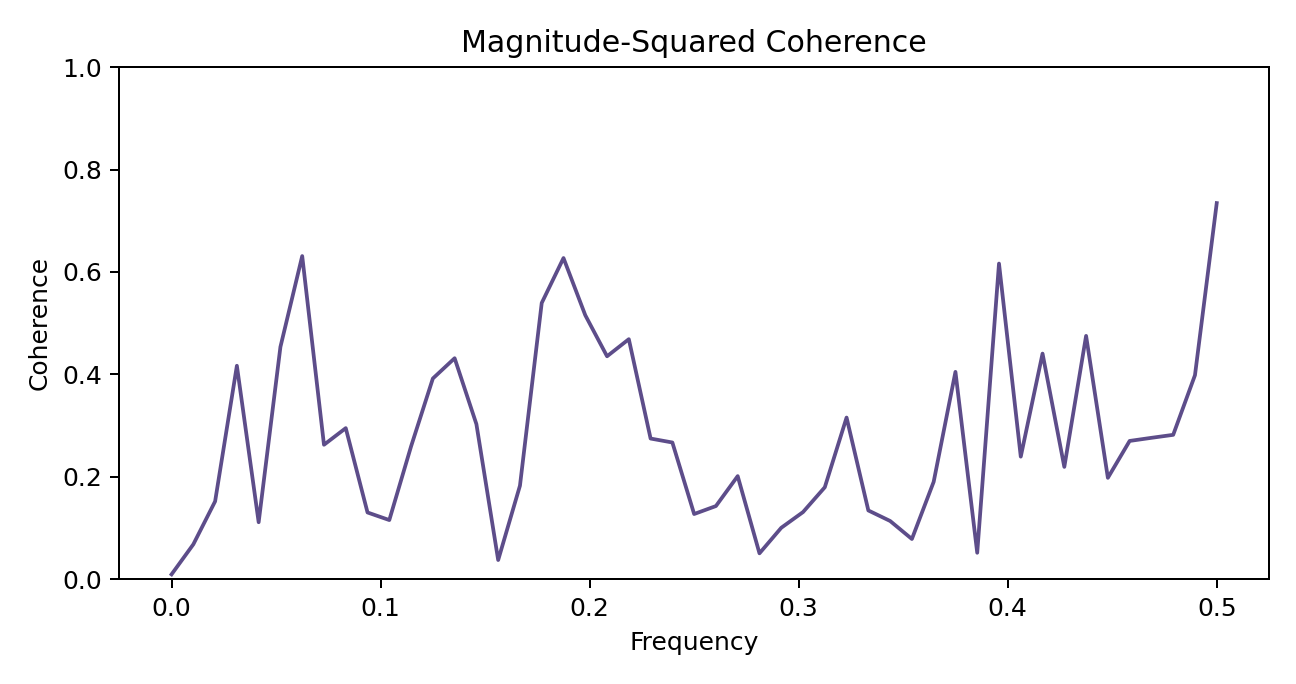
\includegraphics[width=0.86\textwidth]{ch12_fig02_coherence.png}
  \caption{相干性曲线：展示两个序列在不同频率上的线性关联强度。}
\end{figure}

\section{练习提要}

原文练习主要围绕下列方向展开：
\begin{itemize}
  \item 计算二元 VAR 的自协方差矩阵；
  \item 估计交叉谱和相干性；
  \item 解释逆谱密度矩阵零元素；
  \item 比较时域偏相关与频域谱偏相关。
\end{itemize}

\section*{本章小结}

第 12 章把单变量频域理论推广到矩阵情形。多元序列的关键不只是每个变量自身的谱密度，还包括交叉谱、相干性和逆谱密度所揭示的条件依赖网络。

\clearpage
% Source: chapters/ch13_nonlinear_time_series_models/第13章_Nonlinear_Time_Series_Models_非线性时间序列模型.tex
\chapter{Nonlinear Time Series Models / 非线性时间序列模型}
\section*{本章学习目标}

本章按照原文 \textit{Nonlinear Time Series Models} 的小节顺序整理，保留主要定义、定理、模型公式和练习方向，并将原文中的 R 实践思路改写为 Python 工程实践。

完成本章后，应能够：
\begin{itemize}
  \item 理解非线性递推模型的平稳解条件；
  \item 用金融数据动机说明波动聚集；
  \item 掌握 ARCH、GARCH、IGARCH 模型；
  \item 理解双线性模型和随机系数 AR；
  \item 了解非参数时间序列模型。
\end{itemize}

\section{非线性模型的一般形式}

原文以随机递推方程为入口：
\[
  X_t=F(X_{t-1},\varepsilon_t).
\]
\begin{theorem}[Brandt 定理，原文 Theorem 13.0.1]
在随机映射满足平均收缩等条件时，上述递推存在唯一严格平稳解，并可由过去创新的可测函数表示。
\end{theorem}

该定理为 ARCH、GARCH 和双线性模型的存在性提供统一思路。

\section{数据动机}

金融收益序列常呈现三个特征：收益均值相关弱、平方收益或绝对收益相关强、波动成团出现。线性 ARMA 均值模型难以解释这种条件方差变化，因此需要非线性模型。

\section{ARCH 模型}

ARCH(p) 定义为
\[
  X_t=\sigma_t Z_t,\qquad
  \sigma_t^2=a_0+a_1X_{t-1}^2+\cdots+a_pX_{t-p}^2,
\]
其中 \(Z_t\) 通常为 iid 标准化创新。若 \(a_i\ge0\)，可保证条件方差非负。

\subsection{ARCH 的特征}

虽然 \(X_t\) 可不相关，但 \(X_t^2\) 相关，因此模型能刻画波动聚集。

\section{GARCH 模型}

GARCH(1,1) 为
\[
  X_t=\sigma_tZ_t,\qquad
  \sigma_t^2=a_0+a_1X_{t-1}^2+b_1\sigma_{t-1}^2.
\]
若 \(a_1+b_1<1\)，常见二阶平稳条件成立，且
\[
  E(X_t^2)=\frac{a_0}{1-a_1-b_1}.
\]

\begin{example}[GARCH(1,1) 反演，原文 Example 13.3.1]
当 \(b_1<1\) 时，\(\sigma_t^2\) 可展开为过去平方收益的无限加权和，权重按 \(b_1\) 衰减。
\end{example}

\begin{definition}[IGARCH，原文 Definition 13.3.1]
若 GARCH 模型满足 \(a_1+b_1=1\)，称为 IGARCH。此时波动冲击具有极强持续性。
\end{definition}

\section{双线性模型与非参数模型}

双线性模型包含过去观测和过去创新的乘积项，例如
\[
  X_t=\phi X_{t-1}+\theta\varepsilon_{t-1}
      +bX_{t-1}\varepsilon_{t-1}+\varepsilon_t.
\]
它比线性 ARMA 更灵活，可产生非线性依赖。

非参数时间序列模型则把条件均值或条件方差写成未知函数：
\[
  X_t=m(X_{t-1},\ldots,X_{t-p})+\varepsilon_t,
\]
再用核方法、局部线性、样条或机器学习方法估计 \(m\)。原文将其作为高级扩展。

\section{原文数据与模型补充}

\subsection{Yahoo 和 FTSE 数据动机}
原文第 13.1 节用 Yahoo 1996--2014 数据和 2014 年 1--8 月 FTSE 100 数据展示金融收益特征：价格序列非平稳，收益序列均值相关弱，但平方收益和绝对收益显示明显聚集。

\subsection{ARCH 的存在性和二阶平稳}
\begin{theorem}[ARCH 平稳性说明]
ARCH(p) 的严格平稳解可由随机递推理论给出；二阶平稳通常要求 ARCH 系数和小于 1。
\end{theorem}

\subsection{GARCH 扩展}
原文第 13.3.2 还提到 GARCH 的扩展形式，例如非对称 GARCH、EGARCH 或含外生变量的条件方差模型，用于刻画杠杆效应和更复杂的波动动态。

\subsection{R 代码与模拟练习}
第 13.3.3 和 13.4.3 给出 R 代码提示。Exercise 13.1 推导 GARCH 条件，Exercise 13.2 模拟 ARCH/GARCH，Exercise 13.3 模拟双线性模型，Exercise 13.4 研究随机系数 AR 模型。

\begin{example}[随机系数 AR]
随机系数 AR 可写为
\[
  X_t=(\phi+\eta_t)X_{t-1}+\varepsilon_t.
\]
即使条件均值类似 AR(1)，随机系数也会带来非线性依赖和时变波动。
\end{example}

\section{Python 工程实践}

在本章目录下运行：
\begin{lstlisting}[language=bash]
python scripts/ch13_generate_figures.py
\end{lstlisting}

脚本会把图像写入本章 \texttt{figures/} 目录。当前图像用于配合本章核心概念的仿真说明；若后续补齐原始数据文件，可把模拟数据替换为原文真实数据案例。

\begin{figure}[htbp]
  \centering
  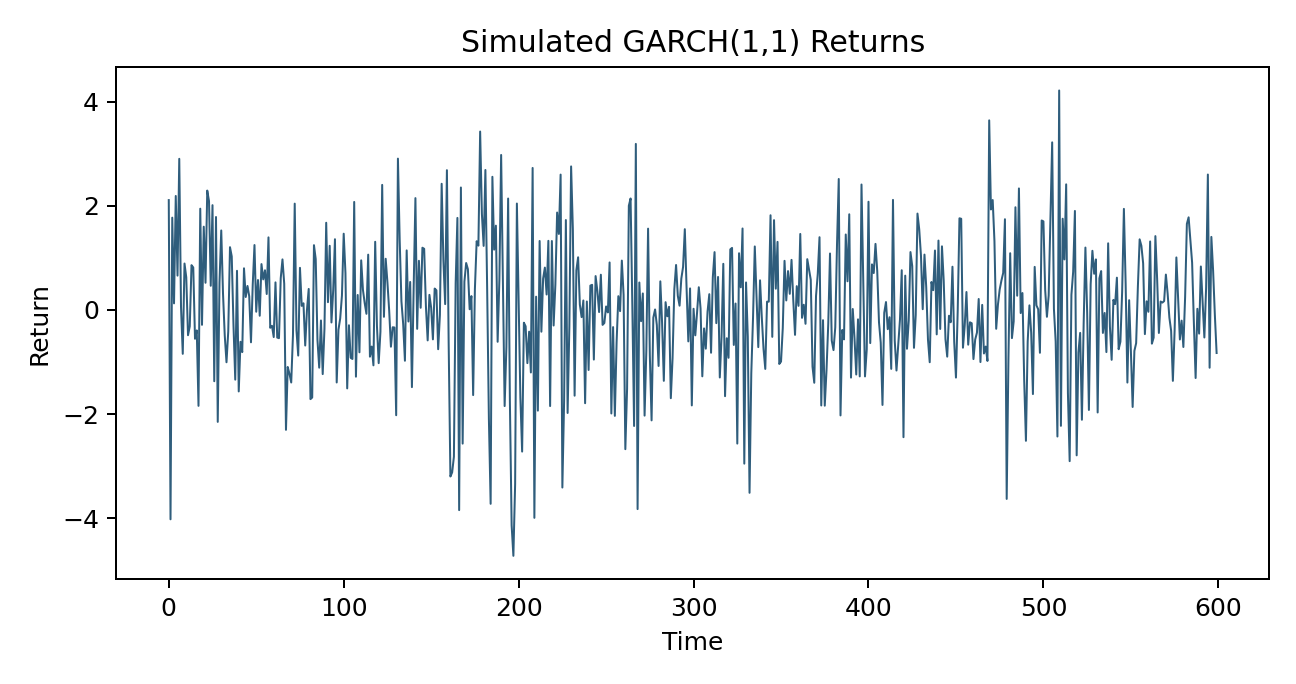
\includegraphics[width=0.86\textwidth]{ch13_fig01_garch_returns.png}
  \caption{GARCH(1,1) 收益模拟：收益本身均值稳定，但波动呈现聚集。}
\end{figure}

\begin{figure}[htbp]
  \centering
  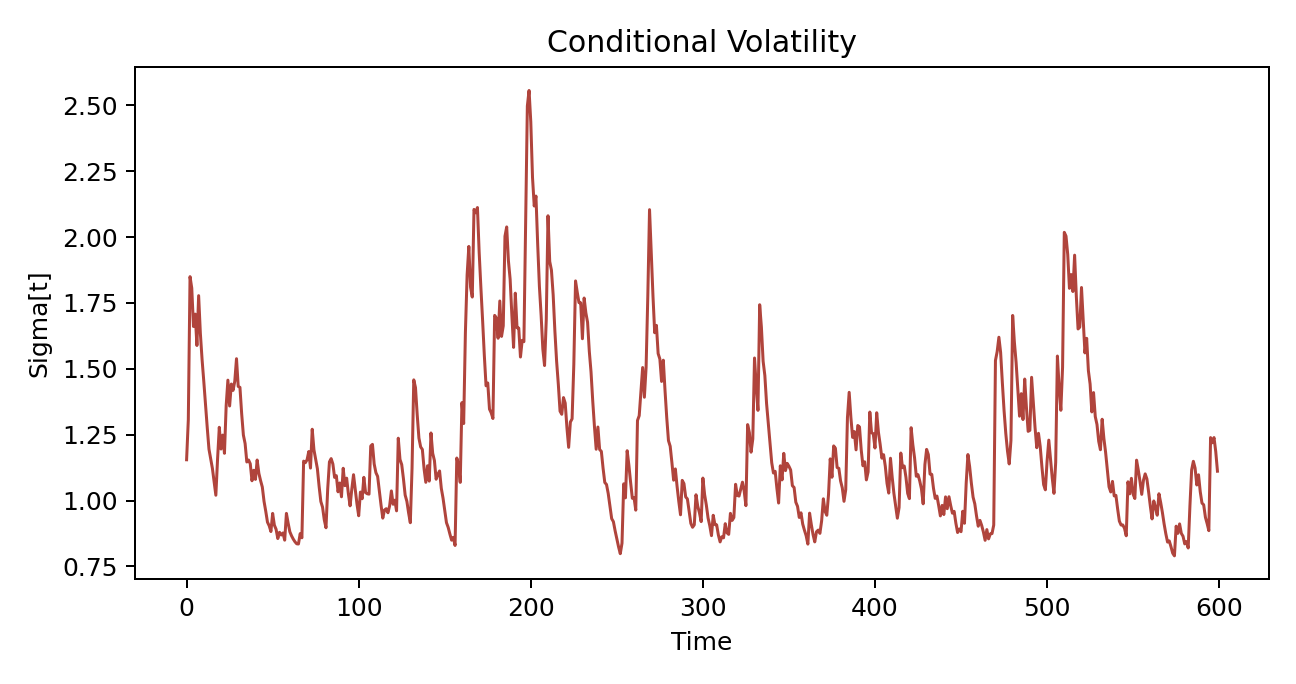
\includegraphics[width=0.86\textwidth]{ch13_fig02_conditional_volatility.png}
  \caption{条件波动率路径：GARCH 模型通过递推方差刻画风险随时间变化。}
\end{figure}

\section{练习提要}

原文练习主要围绕下列方向展开：
\begin{itemize}
  \item 推导 ARCH(1) 二阶平稳条件；
  \item 模拟 ARCH 与 GARCH 并比较 ACF 和平方 ACF；
  \item 分析 IGARCH 的持续性；
  \item 模拟双线性或随机系数 AR 模型。
\end{itemize}

\section*{本章小结}

第 13 章从线性均值模型转向条件方差和非线性依赖。ARCH/GARCH 解释金融数据的波动聚集，双线性和非参数模型则展示了更一般的非线性动态。

\clearpage
% Source: chapters/ch14_consistency_and_asymptotic_normality_of_esti/第14章_Consistency_asymptotic_normality_一致性与渐近正态性.tex
\chapter{Consistency and asymptotic normality / 一致性与渐近正态性}
\section*{本章学习目标}

本章按照原文 \textit{Consistency and asymptotic normality of estimators} 的小节顺序整理，保留主要定义、定理、模型公式和练习方向，并将原文中的 R 实践思路改写为 Python 工程实践。

完成本章后，应能够：
\begin{itemize}
  \item 区分几乎必然收敛、依概率收敛和分布收敛；
  \item 定义估计量的一致性和渐近正态性；
  \item 掌握 argmax/argmin 一致性定理；
  \item 理解随机等连续和随机 Ascoli 引理；
  \item 应用于 Hannan-Rissanen 和高斯 MLE。
\end{itemize}

\section{收敛模式}

\begin{definition}[收敛，原文 Definition 14.1.1]
若 \(X_n\to X\) 几乎处处，记 \(X_n\xrightarrow{a.s.}X\)；若对任意 \(\epsilon>0\)，
\[
  P(|X_n-X|>\epsilon)\to0,
\]
记 \(X_n\xrightarrow{p}X\)；若分布函数收敛，记 \(X_n\Rightarrow X\)。
\end{definition}

\begin{definition}[有界性，原文 Definition 14.1.2]
\(X_n=O_p(1)\) 表示随机变量序列依概率有界，\(X_n=o_p(1)\) 表示依概率收敛到 0。
\end{definition}

\section{抽样性质与一致性}

\begin{definition}[一致估计，原文 Definition 14.2.1]
若估计量 \(\hat a_n\) 满足
\[
  \hat a_n\xrightarrow{a.s.}a_0
\]
或 \(\hat a_n\xrightarrow{p}a_0\)，则分别称为几乎必然一致或依概率一致。
\end{definition}

\section{估计量的几乎必然收敛}

\begin{definition}[一致收敛，原文 Definition 14.3.1]
若
\[
  \sup_{a\in\Theta}|L_n(a)-L(a)|\xrightarrow{a.s.}0,
\]
称 \(L_n\) 几乎必然一致收敛到 \(L\)。
\end{definition}

\begin{theorem}[Argmax 一致性，原文 Theorem 14.3.1]
若 \(\hat a_n=\arg\max L_n(a)\)，\(a_0=\arg\max L(a)\)，且 \(L_n\) 一致收敛到 \(L\)、\(L\) 的最大点唯一，则 \(\hat a_n\to a_0\)。
\end{theorem}

\section{随机等连续与玩具例子}

\begin{definition}[随机等连续，原文 Definition 14.3.2]
随机函数族在参数空间上若小距离参数点的函数值差可一致控制，则称随机等连续。
\end{definition}

\begin{theorem}[随机 Ascoli 引理，原文 Theorem 14.3.2]
若参数空间紧、随机函数点态收敛且随机等连续，则可推出一致收敛。
\end{theorem}

原文用 AR(1) 估计的玩具例子说明如何把样本目标函数写成极限函数加误差项，并证明
\[
  \hat\phi\xrightarrow{a.s.}\phi.
\]

\section{渐近正态性}

若目标函数 \(L_n(\theta)\) 在真值附近可二阶展开，则一阶条件给出
\[
  0=L_n'(\hat\theta)
  =L_n'(\theta_0)+L_n''(\theta_0)(\hat\theta-\theta_0)+R_n.
\]
若
\[
  \sqrt n L_n'(\theta_0)\Rightarrow N(0,V),
  \qquad
  L_n''(\theta_0)\xrightarrow{p}H,
\]
则
\[
  \sqrt n(\hat\theta-\theta_0)\Rightarrow N(0,H^{-1}VH^{-1}).
\]

\section{Hannan-Rissanen 与 GMLE 渐近性质}

原文后半部分把上述工具用于 Hannan-Rissanen 估计和 ARMA 高斯最大似然。核心任务是证明初步 AR 近似误差足够小、目标函数一致收敛，并用 Taylor 展开得到渐近正态性。

\section{原文定理链补充}

\subsection{随机 Ascoli 证明}
\begin{lemma}[原文 Lemma 14.3.1]
若随机函数列点态收敛且随机等连续，则可推出一致收敛。这是随机 Ascoli 定理证明中的关键步骤。
\end{lemma}

\subsection{AR(1) 玩具例子}
\begin{theorem}[原文 Theorem 14.4.1]
对 AR(1) 估计量 \(\hat\phi\)，在稳定和矩条件下有
\[
  \hat\phi\xrightarrow{a.s.}\phi.
\]
该例展示如何用目标函数极值和遍历定理证明强相合。
\end{theorem}

\subsection{Hannan-Rissanen 渐近性质}
\begin{theorem}[原文 Theorem 14.7.1--14.7.2]
在 ARMA 根条件和高阶 AR 近似阶数合适时，Hannan-Rissanen 初步估计满足所需收敛率，并可进入后续渐近正态证明。
\end{theorem}

\begin{theorem}[原文 Theorem 14.7.3]
ARMA 过程的依赖衰减和矩界给出估计误差的几乎必然控制；附录 B 详细证明该技术结果。
\end{theorem}

\subsection{GMLE 渐近性质}
\begin{proposition}[原文 Proposition 14.8.1--14.8.2]
精确预测、截断预测和近似预测对应的高斯似然在大样本下差异可控，因此它们给出的估计量具有相同一阶渐近性质。
\end{proposition}

\begin{theorem}[原文 Theorem 14.8.1--14.8.2]
在 Assumption 14.8.1 等正则条件下，ARMA 高斯最大似然估计量相合，并且精确似然与近似似然估计量渐近等价。
\end{theorem}

\section{Python 工程实践}

在本章目录下运行：
\begin{lstlisting}[language=bash]
python scripts/ch14_generate_figures.py
\end{lstlisting}

脚本会把图像写入本章 \texttt{figures/} 目录。当前图像用于配合本章核心概念的仿真说明；若后续补齐原始数据文件，可把模拟数据替换为原文真实数据案例。

\begin{figure}[htbp]
  \centering
  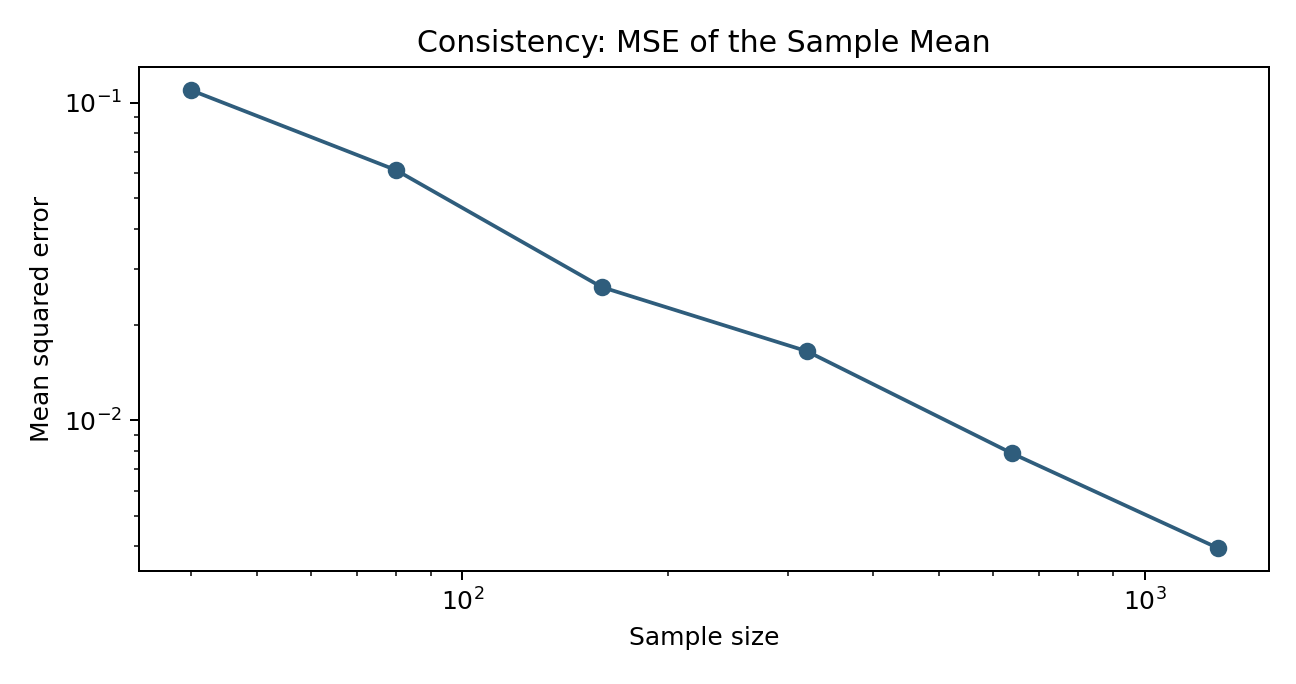
\includegraphics[width=0.86\textwidth]{ch14_fig01_consistency_mse.png}
  \caption{一致性示意：样本量增大时样本均值的均方误差下降。}
\end{figure}

\begin{figure}[htbp]
  \centering
  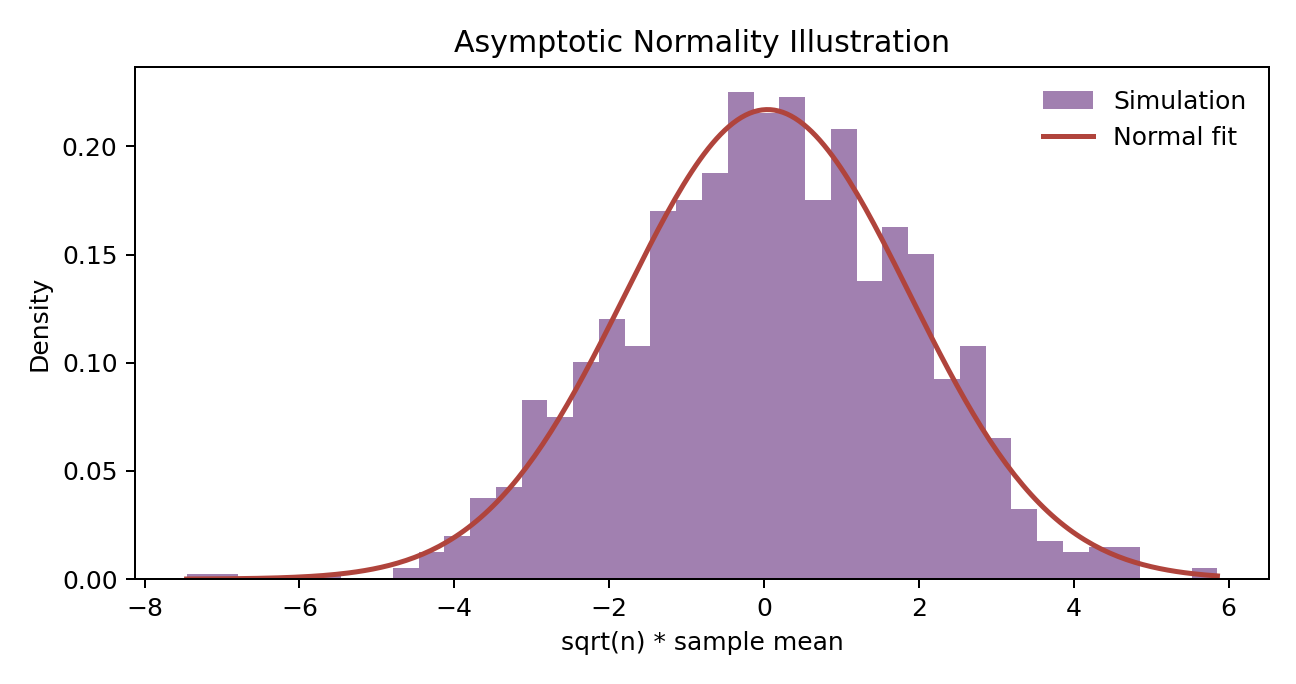
\includegraphics[width=0.86\textwidth]{ch14_fig02_asymptotic_normality.png}
  \caption{渐近正态性示意：标准化估计误差逐渐接近正态分布。}
\end{figure}

\section{练习提要}

原文练习主要围绕下列方向展开：
\begin{itemize}
  \item 判断不同收敛模式之间的关系；
  \item 验证一个目标函数的一致收敛；
  \item 用 AR(1) 估计推导一致性；
  \item 对 M 估计量做 Taylor 展开得到渐近正态。
\end{itemize}

\section*{本章小结}

第 14 章是全书理论证明工具箱。一致性来自目标函数的统一收敛和唯一极值，渐近正态性来自一阶条件、Taylor 展开和中心极限定理；这些工具支撑前面估计方法的抽样性质。

\clearpage
% Source: chapters/ch15_residual_bootstrap_for_estimation_in_autoreg/第15章_Residual_Bootstrap_残差Bootstrap.tex
\chapter{Residual Bootstrap / 残差 Bootstrap}
\section*{本章学习目标}

本章按照原文 \textit{Residual Bootstrap for estimation in autoregressive processes} 的小节顺序整理，保留主要定义、定理、模型公式和练习方向，并将原文中的 R 实践思路改写为 Python 工程实践。

完成本章后，应能够：
\begin{itemize}
  \item 理解 AR 模型残差 Bootstrap 的算法步骤；
  \item 区分真实残差、中心化残差和 bootstrap 残差；
  \item 理解 bootstrap 估计量抽样性质；
  \item 掌握 Wasserstein/分布距离在证明中的作用；
  \item 说明何时 residual bootstrap 能近似参数估计分布。
\end{itemize}

\section{残差 Bootstrap}

对 AR(p)
\[
  X_t=\phi_1X_{t-1}+\cdots+\phi_pX_{t-p}+\varepsilon_t,
\]
先估计 \(\hat\phi\)，得到残差
\[
  \hat\varepsilon_t=X_t-\hat\phi_1X_{t-1}-\cdots-\hat\phi_pX_{t-p}.
\]
中心化后从 \(\{\hat\varepsilon_t-\bar{\hat\varepsilon}\}\) 中有放回抽样，得到 bootstrap 创新 \(\varepsilon_t^+\)，再递推生成
\[
  X_t^+=\hat\phi_1X_{t-1}^++\cdots+\hat\phi_pX_{t-p}^+ + \varepsilon_t^+.
\]
对 bootstrap 样本重新估计参数，重复多次即可近似 \(\hat\phi\) 的抽样分布。

\section{残差 Bootstrap 的抽样性质}

原文通过若干引理证明 bootstrap 残差分布接近真实创新分布，并进一步证明 bootstrap 估计量能近似原估计量的分布。

\begin{lemma}[分布距离，原文 Lemma 15.2.1]
两个概率测度在适当距离 \(d(\alpha,\beta)\) 下收敛，可等价刻画相应随机变量分布的弱收敛。
\end{lemma}

\begin{lemma}[bootstrap 残差，原文 Lemma 15.2.2]
在 AR 参数估计相合和残差中心化条件下，bootstrap 残差的经验分布逼近真实创新分布。
\end{lemma}

\begin{lemma}[bootstrap 序列近似，原文 Lemma 15.2.3--15.2.4]
由 bootstrap 创新递推生成的序列，其样本矩阵和协方差项可逼近理论对应量，从而支持 bootstrap 参数估计的渐近有效性。
\end{lemma}

\section{算法总结}

残差 Bootstrap 的实务步骤为：
\begin{enumerate}
  \item 拟合 AR(p) 并保存参数 \(\hat\phi\)；
  \item 计算并中心化残差；
  \item 重抽样残差生成 \(\varepsilon_t^+\)；
  \item 使用 \(\hat\phi\) 和 \(\varepsilon_t^+\) 递推生成 \(X_t^+\)；
  \item 对 \(X_t^+\) 重新估计，得到 \(\hat\phi^+\)；
  \item 用 \(\hat\phi^+-\hat\phi\) 的经验分布构造标准误、置信区间或分位数。
\end{enumerate}

该方法依赖 AR 模型设定合理、残差近似独立同分布和参数估计稳定。

\section{原文逐段补充与证明细节}

本章开头先回顾前文的渐近抽样理论。前面已经研究过若干估计量的渐近分布，例如自回归参数的最小二乘估计量，以及用于估计 ARMA 参数的高斯最大似然估计量。这些渐近分布可以用于统计检验和置信区间构造。然而，渐近结果只在样本量相对较大时近似有效；当样本量较小时，正态近似可能并不可靠，需要更好的有限样本近似。

即使愿意使用渐近分布，也常常需要估计方差或偏差。有时这些表达式难以推导，或者推导成本很高。Bootstrap 的作用正在于此：它通过从样本本身构造近似分布，来估计估计量的方差、偏差、置信区间等性质。原文引用 Wikipedia 的说法：Bootstrap 是通过从近似分布中抽样，并在这些抽样上测量估计量性质，从而估计估计量性质的一种实践。直观地说，Bootstrap 是“从样本中再抽样”。每一个重抽样样本都被当作来自总体的新样本；利用这些“新的”多个实现，可以近似参数估计量的置信区间和方差。

必须注意，现实中我们并没有真的得到多个独立样本。重复重抽样并不会凭空创造新信息；它只是利用现有样本构造一个近似总体。因此，重抽样次数越多并不等于信息越多，但它能帮助我们理解估计量的有限样本分布。本章将详细说明残差 bootstrap 方法，并证明在渐近意义下，bootstrap 分布与估计量的渐近分布一致。

残差 bootstrap 最早由 J. P. Kreiss 提出，Kreiss (1997) 是一篇很好的综述。Franke and Kreiss (1992) 还给出了对 \(AR(\infty)\) 过程的扩展。早期关于 bootstrap 理论的重要论文包括 Bickel and Freedman (1981)。时间序列中还有其他 bootstrap 方法，例如周期图 bootstrap、block bootstrap、Kalman filter bootstrap 等。这些方法不仅用于估计方差，也可用于确定模型阶数等问题。频域方法可参考 Dahlhaus and Janas (1996) 和 Franke and Härdle (1992)，子抽样方法综述可参考 Politis 等人的工作。

\subsection{残差 bootstrap 的模型假设}

原文设定时间序列 \(\{X_t\}\) 满足平稳、因果的 AR(p) 过程：
\[
  X_t=\sum_{j=1}^p\phi_jX_{t-j}+\varepsilon_t,
\]
其中 \(\{\varepsilon_t\}\) 为 iid 随机变量，均值为 0，方差为 1。AR 特征多项式的根的绝对值都大于 \(1+\delta\)，这意味着过程不仅稳定，而且根与单位圆有正距离。为简化讨论，原文假定阶数 \(p\) 已知。

定义滞后向量
\[
  X_{t-1}'=(X_{t-1},\ldots,X_{t-p}).
\]
第一步构造样本矩阵和样本向量：
\[
  \hat\Gamma_p=\frac1n\sum_{t=p+1}^nX_{t-1}X_{t-1}',
  \qquad
  \hat\gamma_p=\frac1n\sum_{t=p+1}^nX_{t-1}X_t.
  \tag{15.1}
\]
于是自回归参数估计量写作
\[
  \hat\phi_n=(\hat\phi_1,\ldots,\hat\phi_p)'
  =\hat\Gamma_p^{-1}\hat\gamma_p.
\]
这正是条件最小二乘或 Yule-Walker 型回归估计的矩阵写法。

第二步估计残差：
\[
  \hat\varepsilon_t=X_t-\sum_{j=1}^p\hat\phi_jX_{t-j}.
\]
第三步用这些估计残差构造经验分布函数：
\[
  \hat F_n(x)
  =\frac1{n-p}\sum_{t=p+1}^n I_{(-\infty,\hat\varepsilon_t]}(x).
\]
从 \(\hat F_n\) 抽样等价于：以概率 \((n-p)^{-1}\) 从每一个估计残差 \(\hat\varepsilon_t\) 中抽取一个值。

第四步，从 \(\hat F_n\) 独立抽取 \(n\) 个 bootstrap 创新，记为 \(\{\varepsilon_k^+\}\)。第五步，给定初始值 \(X_k^+=\varepsilon_k^+\)（\(1\le k\le p\)），对 \(k>p\) 用
\[
  X_k^+=\sum_{j=1}^p\hat\phi_jX_{k-j}^+ + \varepsilon_k^+
\]
递推生成 bootstrap 序列。第六步，重复该过程 \(N\) 次，得到 \(N\) 个 bootstrap 样本。第七步，对每个 bootstrap 样本重新计算 \(\Gamma_p^+\)、\(\gamma_p^+\) 和
\[
  \hat\phi_n^+=(\Gamma_p^+)^{-1}\gamma_p^+.
\]
第八步，用这些 \(\hat\phi_n^+\) 的经验分布估计 \(\hat\phi_n-\phi\) 的分布，或者估计 \(\hat\phi_n\) 的方差。

\subsection{bootstrap 抽样性质的目标}

第 15.2 节要证明：
\[
  \sqrt n(\hat\phi_n^+-\hat\phi_n)
\]
的分布与
\[
  \sqrt n(\hat\phi_n-\phi)
\]
的分布渐近一致。这说明在大样本极限下，使用 bootstrap 分布不会比使用渐近正态近似更差。原文同时提醒：这个结论并不自动说明 bootstrap 分布对有限样本分布的近似一定优于普通正态近似。若要比较更高阶精度，需要使用 Edgeworth 展开等工具。

为了证明两个分布渐近一致，原文使用如下距离。对 \(p>1\)，定义
\[
  d_p(H,G)=\inf_{X\sim H,Y\sim G}\{E|X-Y|^p\}^{1/p}.
\]
这里下确界取遍所有边际分布分别为 \(H\) 和 \(G\) 的联合分布。当 \(p=2\) 时，该距离称为 Mallows 距离：
\[
  d_2(H,G)=\inf_{X\sim H,Y\sim G}\{E|X-Y|^2\}^{1/2}.
\]
如果 \(H=G\)，可取 \(X=Y\)，于是距离为 0。为了简化记号，原文把随机变量的边际分布记入符号中，写作 \(d_p(X,Y)\)。该距离满足三角不等式。

\begin{lemma}[Mallows 距离与弱收敛，原文 Lemma 15.2.1]
设 \(\alpha_n\) 和 \(\alpha\) 为两个概率测度，则
\[
  d_p(\alpha_n,\alpha)\to0
\]
当且仅当 \(\alpha_n\) 弱收敛到 \(\alpha\)，并且 \(p\) 阶绝对矩收敛：
\[
  \int |x|^p\alpha_n(dx)\to \int |x|^p\alpha(dx).
\]
\end{lemma}

本章的目标可写为
\[
  d_2\{\sqrt n(\hat\phi_n^+-\hat\phi_n),
      \sqrt n(\hat\phi_n-\phi)\}\to0.
\]
若该式成立，则两者的极限分布相同。

证明中反复使用两个展开：
\[
  \sqrt n(\hat\phi_n-\phi)
  =\sqrt n\,\hat\Gamma_p^{-1}(\hat\gamma_p-\hat\Gamma_p\phi),
\]
以及
\[
  \sqrt n(\hat\phi_n^+-\hat\phi_n)
  =\sqrt n\,(\Gamma_p^+)^{-1}(\gamma_p^+-\Gamma_p^+\hat\phi_n).
\]
因此关键是比较 \(\hat\Gamma_p,\hat\gamma_p\) 与它们的 bootstrap 对应量 \(\Gamma_p^+,\gamma_p^+\)。

\subsection{估计残差分布逼近真实创新分布}

\begin{lemma}[估计残差与真实残差的距离，原文 Lemma 15.2.2]
设 \(\varepsilon_t^+\) 为 bootstrap 残差，\(\varepsilon_t\) 为真实创新。令离散随机变量 \(J\) 在集合 \(\{p+1,\ldots,n\}\) 上均匀取值，即
\[
  P(J=k)=\frac1{n-p}.
\]
则
\[
  E\{(\hat\varepsilon_J-\varepsilon_J)^2\mid X_1,\ldots,X_n\}
  =O_p(n^{-1}),
  \tag{15.2}
\]
并且
\[
  d_2(\hat F_n,F)
  \le d_2(\hat F_n,F_n)+d_2(F_n,F)\to0,
  \tag{15.3}
\]
其中 \(F_n\) 是真实创新 \(\{\varepsilon_t\}\) 的经验分布，\(\hat F_n\) 是估计残差的经验分布，\(F\) 是真实创新分布。
\end{lemma}

证明的第一步是展开残差差：
\[
  \hat\varepsilon_t-\varepsilon_t
  =\sum_{j=1}^p(\hat\phi_j-\phi_j)X_{t-j}.
\]
于是条件均方误差为
\[
  \frac1{n-p}\sum_{t=p+1}^n
  \left\{\sum_{j=1}^p(\hat\phi_j-\phi_j)X_{t-j}\right\}^2.
\]
继续展开为双重求和：
\[
  \sum_{j_1,j_2=1}^p(\hat\phi_{j_1}-\phi_{j_1})
  (\hat\phi_{j_2}-\phi_{j_2})
  \frac1{n-p}\sum_{t=p+1}^nX_{t-j_1}X_{t-j_2}.
\]
利用前一章的估计量收敛率
\[
  \sup_{1\le j\le p}|\hat\phi_j-\phi_j|=O_p(n^{-1/2}),
\]
以及样本二阶矩有界，可得 (15.2)。

证明 (15.3) 时，原文先用三角不等式：
\[
  d_2(\hat F_n,F)\le d_2(\hat F_n,F_n)+d_2(F_n,F).
\]
Bickel and Freedman 的结果给出 \(d_2(F_n,F)\to0\)。剩下只需证明 \(d_2(\hat F_n,F_n)\to0\)。为此，构造一个强相关耦合：让从 \(\hat F_n\) 抽到的变量为 \(\hat\varepsilon_J\)，从 \(F_n\) 抽到的变量为 \(\varepsilon_J\)。在该联合分布下，
\[
  d_2(\hat F_n,F_n)^2
  \le E\{(\hat\varepsilon_J-\varepsilon_J)^2\mid X_1,\ldots,X_n\}
  =O_p(n^{-1}).
\]
于是估计残差经验分布在 Mallows 距离下逼近真实创新分布。

\begin{proposition}[二阶矩一致性，原文 Corollary 15.2.1]
若 \(\varepsilon_t^+\) 从 bootstrap 残差分布抽取，则
\[
  E_{\hat F_n}\{(\varepsilon_t^+)^2\mid X_1,\ldots,X_n\}
  \xrightarrow{p} E_F(\varepsilon_t^2).
\]
\end{proposition}

该结论直接由 Lemma 15.2.1 和 Lemma 15.2.2 得到。它说明 bootstrap 创新的方差渐近等于真实创新方差。

\subsection{bootstrap 序列与真实序列的近似}

由于 \(X_t\) 是因果 AR 过程，存在系数 \(\{a_j\}\)，使得
\[
  X_t=\sum_{j=0}^{\infty}a_j\varepsilon_{t-j},
\]
其中 \(a_j=a_j(\phi)\)，并且这些系数几何衰减。使用估计参数 \(\hat\phi_n\) 时，bootstrap 序列可写为
\[
  X_t^+=\sum_{j=0}^{t}a_j(\hat\phi_n)\varepsilon_{t-j}^+.
\]
原文接下来证明 \(X_t^+\) 与 \(X_t\) 在 Mallows 距离下接近。

\begin{lemma}[bootstrap 线性表示的三段近似，原文 Lemma 15.2.3]
令 \(J_{p+1},\ldots,J_n\) 为从 \(\{p+1,\ldots,n\}\) 中独立均匀抽样得到的指标。定义
\[
  Y_t^+=\sum_{j=p+1}^t a_j(\hat\phi_n)\hat\varepsilon_{J_{t-j}},
\]
\[
  \widetilde Y_t^+=\sum_{j=p+1}^t a_j(\hat\phi_n)\varepsilon_{J_{t-j}},
\]
\[
  \widetilde Y_t=\sum_{j=p+1}^t a_j\varepsilon_{J_{t-j}},
  \qquad
  Y_t=\widetilde Y_t+\sum_{j=t+p+1}^{\infty}a_j\varepsilon_{t-j}.
\]
则有三类误差界：
\[
  E\{(Y_t^+-\widetilde Y_t^+)^2\mid X_1,\ldots,X_n\}=O_p(n^{-1}),
  \tag{15.4}
\]
\[
  E\{(\widetilde Y_t^+-\widetilde Y_t)^2\mid X_1,\ldots,X_n\}=O_p(n^{-1}),
  \tag{15.5}
\]
以及
\[
  E\{(\widetilde Y_t-Y_t)^2\mid X_1,\ldots,X_n\}\le K\rho^t.
  \tag{15.6}
\]
\end{lemma}

这三个界分别对应三种误差来源。第一，使用估计参数 \(\hat\phi_n\) 替代真实参数 \(\phi\) 带来的误差。由于 \(\hat\phi_n-\phi=O_p(n^{-1/2})\)，且伴随矩阵幂 \(A(\phi)^j\) 几何衰减，所以累积误差仍为 \(O_p(n^{-1})\) 量级。第二，使用估计残差替代真实创新带来的误差，这由 Lemma 15.2.2 控制。第三，把无限线性过程截断为有限和带来的尾部误差；由于 AR 根离单位圆有距离，系数几何衰减，因此尾部误差被 \(K\rho^t\) 控制。

原文证明 (15.4) 时先写出
\[
  E\{(Y_t^+-\widetilde Y_t^+)^2\mid X_1,\ldots,X_n\}
  \le
  \sum_{j=0}^t
  \left([A(\phi)^j]_{1,1}-[A(\hat\phi_n)^j]_{1,1}\right)^2
  E\{(\varepsilon_j^+)^2\mid X_1,\ldots,X_n\}.
\]
再用均值定理和矩阵幂的几何衰减，得到
\[
  |[A(\phi)^j-A(\hat\phi_n)^j]_{1,1}|
  \le K n^{-1/2}\rho^j.
\]
代回求和即可得到 \(O_p(n^{-1})\)。证明 (15.5) 直接使用 Lemma 15.2.2；证明 (15.6) 使用线性系数尾和的几何衰减。

\subsection{矩阵和向量项的近似}

由估计公式可知
\[
  \hat\gamma_p-\hat\Gamma_p\phi
  =\frac1{n-p}\sum_{t=p+1}^n\varepsilon_tX_{t-1},
\]
而 bootstrap 对应量为
\[
  \gamma_p^+-\Gamma_p^+\hat\phi_n
  =\frac1{n-p}\sum_{t=p+1}^n\varepsilon_t^+X_{t-1}^+.
  \tag{15.10}
\]
因此只要证明上式两边在 \(\sqrt n\) 缩放后分布接近，并且 \(\Gamma_p^+\) 与 \(\hat\Gamma_p\) 接近，就能得到参数估计量分布接近。

\begin{lemma}[矩阵、向量与估计方程近似，原文 Lemma 15.2.4]
令 \(Y_t,Y_t^+,\widetilde Y_t,\widetilde Y_t^+\) 如 Lemma 15.2.3 所定义，并用它们构造 \(\bar\Gamma_p,\bar\Gamma_p^+,\bar\gamma_p,\bar\gamma_p^+\)。则
\[
  d_2(Y_t,Y_t^+)\le \{E(Y_t-Y_t^+)^2\}^{1/2}
  =O_p(n^{-1/2}+\rho^t),
  \tag{15.11}
\]
\[
  d_2(Y_t,X_t)\to0,
  \tag{15.12}
\]
并且
\[
  d_2\{\sqrt n(\bar\gamma_p-\bar\Gamma_p\phi),
        \sqrt n(\bar\gamma_p^+-\bar\Gamma_p^+\hat\phi_n)\}\to0.
  \tag{15.13}
\]
此外，
\[
  E|\bar\Gamma_p^+-\bar\Gamma_p|\to0,
  \tag{15.14}
\]
以及
\[
  d_2\{(\bar\gamma_p-\bar\Gamma_p\phi),
       (\gamma_p-\Gamma_p\phi)\}\to0,\qquad
  E|\bar\Gamma_p-\hat\Gamma_p|\to0.
  \tag{15.15}
\]
\end{lemma}

证明 (15.11) 使用 Lemma 15.2.3 中的三角不等式。也就是说，\(Y_t\) 与 \(Y_t^+\) 的差可以拆成尾部截断误差、参数估计误差和残差替换误差三部分，每一部分都有界。证明 (15.12) 的关键是：\(Y_t\) 与 \(X_t\) 的差别只在于 \(Y_t\) 使用从经验分布中抽到的创新，而 \(X_t\) 使用真实 iid 创新；由于经验分布 \(F_n\) 在 Mallows 距离下收敛到 \(F\)，两者距离趋于 0。

证明 (15.13) 时，原文比较
\[
  (\bar\gamma_p-\bar\Gamma_p\phi)
  -(\bar\gamma_p^+-\bar\Gamma_p^+\hat\phi_n).
\]
利用 (15.10)，该差可写成
\[
  \frac1n\sum_{t=p+1}^n
  \left\{(\varepsilon_t-\varepsilon_t^+)Y_{t-1}
  +\varepsilon_t^+(Y_{t-1}-Y_{t-1}^+)\right\}.
\]
条件在 \(X_1,\ldots,X_n\) 上，\(\varepsilon_t-\varepsilon_t^+\) 与过去项独立，于是可分别控制两项。第一项由 Lemma 15.2.2 给出 \(O(n^{-1/2})\)；第二项由 Corollary 15.2.1 和 (15.11) 控制，也为 \(O(n^{-1/2})\)。于是得到 (15.13)。矩阵项 (15.14) 和 (15.15) 可用类似方式证明。

\begin{proposition}[样本矩阵和估计方程的最终近似，原文 Corollary 15.2.2]
令 \(\Gamma_p^+,\hat\Gamma_p,\hat\gamma_p,\gamma_p^+\) 如 (15.1) 及 bootstrap 定义所示，则
\[
  d_2\{\sqrt n(\hat\gamma_p-\hat\Gamma_p\phi),
        \sqrt n(\gamma_p^+-\Gamma_p^+\hat\phi_n)\}\to0,
  \tag{15.16}
\]
并且
\[
  d_1(\Gamma_p^+,\hat\Gamma_p)\to0.
  \tag{15.17}
\]
\end{proposition}

证明直接由 Lemma 15.2.4、三角不等式以及前面各项近似得到。

\subsection{最终渐近结论}

由 (15.17) 和 Lemma 15.2.1 可得
\[
  \Gamma_p^+\xrightarrow{p}E(\Gamma_p).
\]
由 (15.16) 可知
\[
  \sqrt n(\gamma_p^+-\Gamma_p^+\hat\phi_n)
\]
的分布弱收敛到
\[
  \sqrt n(\hat\gamma_p-\hat\Gamma_p\phi)
\]
的极限分布。因此，
\[
  \sqrt n(\hat\phi_n^+-\hat\phi_n)
  \Rightarrow N(0,2\Gamma_p^{-1})
\]
在原文的方差归一化设定下成立。结合前文结果
\[
  \sqrt n(\hat\phi_n-\phi)
  \Rightarrow N(0,\sigma^2\Gamma_p^{-1}),
\]
可知
\[
  \sqrt n(\hat\phi_n^+-\hat\phi_n)
\]
和
\[
  \sqrt n(\hat\phi_n-\phi)
\]
的分布渐近一致。换言之，残差 bootstrap 在一阶渐近意义下能够正确复现 AR 参数估计量的抽样分布。

从应用角度看，本章结论说明：当 AR 阶数正确、过程稳定且残差能够合理代表创新分布时，可以用 residual bootstrap 近似参数估计量的有限样本不确定性。实际使用时仍需检查残差是否近似 iid、模型阶数是否合适，以及重抽样样本量是否足够。

\subsection{逐页校订补充：从算法到定理的逻辑链}

为了避免把本章误读为纯算法章节，需要把原文的逻辑顺序再完整串联一次。第一个问题是：为什么要从残差中抽样，而不是直接从观测值中抽样？对时间序列来说，原始观测 \(X_t\) 之间相关，直接有放回抽样会破坏时间顺序和依赖结构。AR 模型的建模假设告诉我们，相关结构主要由递推
\[
  X_t=\sum_{j=1}^p\phi_jX_{t-j}+\varepsilon_t
\]
产生，而创新 \(\varepsilon_t\) 是 iid。因此，合理的重抽样对象不是 \(X_t\)，而是拟合模型后的残差 \(\hat\varepsilon_t\)。重抽样残差，再用估计出的 AR 递推重新生成序列，可以同时保留模型中的时间依赖结构和创新分布的非参数近似。

第二个问题是：为什么原文要求 AR 特征根的绝对值大于 \(1+\delta\)，而不只是大于 1？根在单位圆外保证因果平稳；与单位圆有固定距离则给出更强的几何衰减界。后续证明中多次使用
\[
  |a_j|\le K\rho^j,\qquad 0<\rho<1,
\]
以及矩阵幂 \(A(\phi)^j\) 的收缩性质。如果根太接近单位圆，衰减会很慢，有限样本中的 bootstrap 近似会变差，理论证明也需要更精细的局部单位根分析。

第三个问题是：为什么使用 Mallows 距离而不是只讨论弱收敛？弱收敛只能说明分布函数在连续点收敛，却不直接控制矩。参数估计量的渐近分布和 bootstrap 分布不仅需要形状接近，还需要二阶矩、方差等量接近。Mallows 距离 \(d_2\) 同时包含分布收敛和二阶矩收敛，正好适合 bootstrap 方差近似。Lemma 15.2.1 的作用就是把“距离趋于 0”转换成“弱收敛加矩收敛”，从而让后续证明可以通过均方界完成。

第四个问题是：Lemma 15.2.2 为什么是全章的起点？残差 bootstrap 能否正确，首先取决于估计残差分布是否接近真实创新分布。若
\[
  \hat\varepsilon_t-\varepsilon_t
  =\sum_{j=1}^p(\hat\phi_j-\phi_j)X_{t-j}
\]
在均方意义下很小，那么从 \(\hat\varepsilon_t\) 的经验分布抽样与从 \(\varepsilon_t\) 的经验分布抽样就接近。再利用真实创新经验分布 \(F_n\) 收敛到真实分布 \(F\)，得到 \(\hat F_n\to F\)。这一步把估计残差与真实创新连接起来，是后续构造 bootstrap 序列的基础。

第五个问题是：Lemma 15.2.3 为什么要引入 \(Y_t^+\)、\(\widetilde Y_t^+\)、\(\widetilde Y_t\)、\(Y_t\) 四个看似复杂的变量？这是一个分步替换策略。直接比较 \(X_t^+\) 和 \(X_t\) 很困难，因为二者同时差在参数、创新和无限尾项上。原文把差异拆成三步：先把估计参数换成真实参数，再把估计残差换成真实创新，最后处理无限线性表示的尾部。每一步都能用已有界控制，最终用三角不等式合并。

这四个变量的含义可这样理解。\(Y_t^+\) 是最接近 bootstrap 世界的量：它使用估计参数和估计残差。 \(\widetilde Y_t^+\) 仍使用估计参数，但把估计残差换成真实创新的经验抽样。 \(\widetilde Y_t\) 使用真实参数和真实创新经验抽样。 \(Y_t\) 再补上真实线性过程的无限尾项，使其接近真实 \(X_t\)。这种“搭桥”方法在 bootstrap 理论中很常见，因为它能避免一次性比较两个结构差异太大的对象。

第六个问题是：为什么 (15.10) 很重要？参数估计误差可以写成估计方程的形式：
\[
  \hat\gamma_p-\hat\Gamma_p\phi
  =\frac1{n-p}\sum_{t=p+1}^n\varepsilon_tX_{t-1}.
\]
这表示估计误差的主随机项是“创新乘以过去状态”的平均。bootstrap 世界中对应的是
\[
  \gamma_p^+-\Gamma_p^+\hat\phi_n
  =\frac1{n-p}\sum_{t=p+1}^n\varepsilon_t^+X_{t-1}^+.
\]
如果这两个平均项在 \(\sqrt n\) 缩放下分布接近，并且矩阵 \(\Gamma_p^+\) 与 \(\hat\Gamma_p\) 接近，那么由连续映射和矩阵逆的稳定性可得到参数估计量本身的分布接近。

第七个问题是：Lemma 15.2.4 具体完成了什么？它把前面单个时间点的近似提升为样本平均、协方差矩阵和估计方程的近似。证明中条件在原始样本 \(X_1,\ldots,X_n\) 上，利用 bootstrap 创新的条件独立性，将均方误差分解为两项：
\[
  I=\text{残差创新差异项},\qquad
  II=\text{bootstrap 序列状态差异项}.
\]
第一项由 Lemma 15.2.2 控制，第二项由 Lemma 15.2.3 和 Corollary 15.2.1 控制。这样就把“残差分布接近”和“生成序列接近”转化为“估计方程接近”。

第八个问题是：最终结论中的方差形式如何理解？在真实样本中，
\[
  \sqrt n(\hat\phi_n-\phi)
\]
的极限分布由创新方差和滞后向量协方差矩阵决定。若创新方差记作 \(\sigma^2\)，极限协方差一般写成
\[
  \sigma^2\Gamma_p^{-1}.
\]
bootstrap 估计量
\[
  \sqrt n(\hat\phi_n^+-\hat\phi_n)
\]
条件在样本上有一个随机分布；定理说明这个条件分布在渐近上逼近真实估计误差的极限分布。因此，实际构造置信区间时，可以用许多次 \(\hat\phi_n^{+(b)}-\hat\phi_n\) 的经验分位数近似真实误差分位数。

\subsection{残差 bootstrap 的实际实现细节}

真实计算时通常会对残差做中心化。原因是 AR 模型假设创新均值为 0，但有限样本残差均值不一定正好为 0。若直接重抽样未中心化残差，bootstrap 序列可能带有额外均值偏移。中心化做法为
\[
  \tilde\varepsilon_t=\hat\varepsilon_t-\bar{\hat\varepsilon},
  \qquad
  \bar{\hat\varepsilon}=\frac1{n-p}\sum_{t=p+1}^n\hat\varepsilon_t.
\]
然后从 \(\{\tilde\varepsilon_{p+1},\ldots,\tilde\varepsilon_n\}\) 中有放回抽样。

初始值的处理也会影响有限样本结果。原文为了理论简洁，令前 \(p\) 个 bootstrap 值由 bootstrap 创新给出；实际中也常见另一种做法：直接使用原始序列的前 \(p\) 个观测作为初始值，或者先生成较长序列并丢弃 burn-in。只要 AR 模型稳定，初始值影响会随时间衰减；但在小样本或近单位根时，这种影响不可忽略。

重抽样次数 \(N\) 需要足够大。若只估计标准误，几百次可能已经可用；若要估计 2.5\% 和 97.5\% 分位数，通常需要更多重复次数。bootstrap 误差来自两部分：一是样本本身对总体的近似误差，二是有限重抽样次数带来的 Monte Carlo 误差。增加 \(N\) 只能减少第二部分，不能消除样本信息不足带来的误差。

模型阶数 \(p\) 在本章理论中被假设为已知。实际中 \(p\) 往往由 AIC、BIC、PACF 或交叉验证选择。若阶数选择错误，残差可能仍有相关性，bootstrap 创新 iid 的近似就会失败。因此，使用 residual bootstrap 前应检查残差 ACF、PACF 和 Ljung-Box 检验结果。如果残差中仍有显著自相关，应重新建模，而不是直接相信 bootstrap 区间。

残差 bootstrap 与 block bootstrap 的区别也值得说明。Block bootstrap 直接对原始序列的连续块重抽样，适用于更一般的弱依赖过程；它不需要指定 AR 模型，但块长选择很关键。Residual bootstrap 则依赖一个已拟合模型，若模型正确，效率通常更高，并且能保留 AR 递推结构。两者各有适用场景：模型可信时用 residual bootstrap；模型结构不明确但希望保留局部依赖时，用 block bootstrap。

\subsection{本章结论的适用范围与限制}

本章证明的是一阶渐近有效性。也就是说，当 \(n\to\infty\) 时，bootstrap 分布和真实估计误差分布有相同的极限。它并不保证在所有有限样本中 bootstrap 都更准确。若要证明 bootstrap 具有更高阶精度，需要比较 Edgeworth 展开中的高阶项，这超出了本章范围。

本章还依赖 iid 创新假设。如果创新存在条件异方差，例如真实过程为 AR-GARCH，那么简单 residual bootstrap 会把异方差结构打散。此时应考虑 wild bootstrap、sieve bootstrap 或针对 GARCH 的 bootstrap 方法。类似地，如果创新分布有很重的尾部，二阶矩条件可能失败，Mallows 距离和方差估计也需要修改。

另外，本章理论是在平稳因果 AR 模型下展开。若过程存在单位根、结构突变或长记忆，残差 bootstrap 的性质会发生变化。单位根模型下，参数估计量的极限分布通常不是正态，简单按平稳 AR 理论重抽样可能得到错误结论。结构突变会使残差混合来自不同机制，长记忆会导致相关衰减太慢，这些都需要专门方法处理。

因此，正确使用本章方法的流程应是：先用图形、ACF/PACF 和信息准则选择并拟合 AR 模型；再检查残差是否近似 iid；然后实施 residual bootstrap；最后把 bootstrap 区间与渐近正态区间一起报告，并解释两者差异。如果 bootstrap 分布明显偏斜或重尾，应优先使用分位数区间或 studentized bootstrap，而不是只报告正态近似标准误。

从课程结构看，第 15 章把前面多个主题连接起来：第 4 章提供 AR 因果表示，第 8 章提供样本矩和协方差估计，第 9 章提供参数估计，第 14 章提供一致性和渐近正态性证明工具。本章的 residual bootstrap 则把这些理论转化为一种可操作的有限样本近似方法。

\section{Python 工程实践}

在本章目录下运行：
\begin{lstlisting}[language=bash]
python scripts/ch15_generate_figures.py
\end{lstlisting}

脚本会把图像写入本章 \texttt{figures/} 目录。当前图像用于配合本章核心概念的仿真说明；若后续补齐原始数据文件，可把模拟数据替换为原文真实数据案例。

\begin{figure}[htbp]
  \centering
  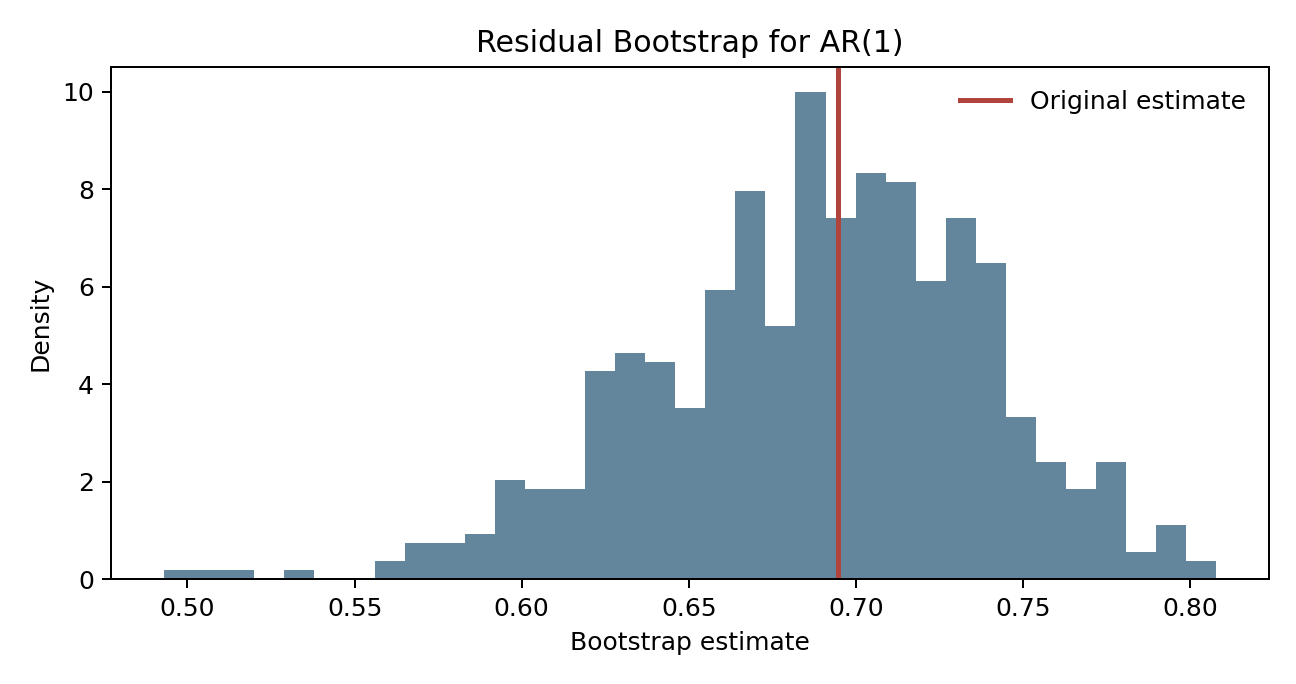
\includegraphics[width=0.86\textwidth]{ch15_fig01_residual_bootstrap.png}
  \caption{AR(1) 残差 Bootstrap 参数分布：重抽样近似估计量的不确定性。}
\end{figure}

\begin{figure}[htbp]
  \centering
  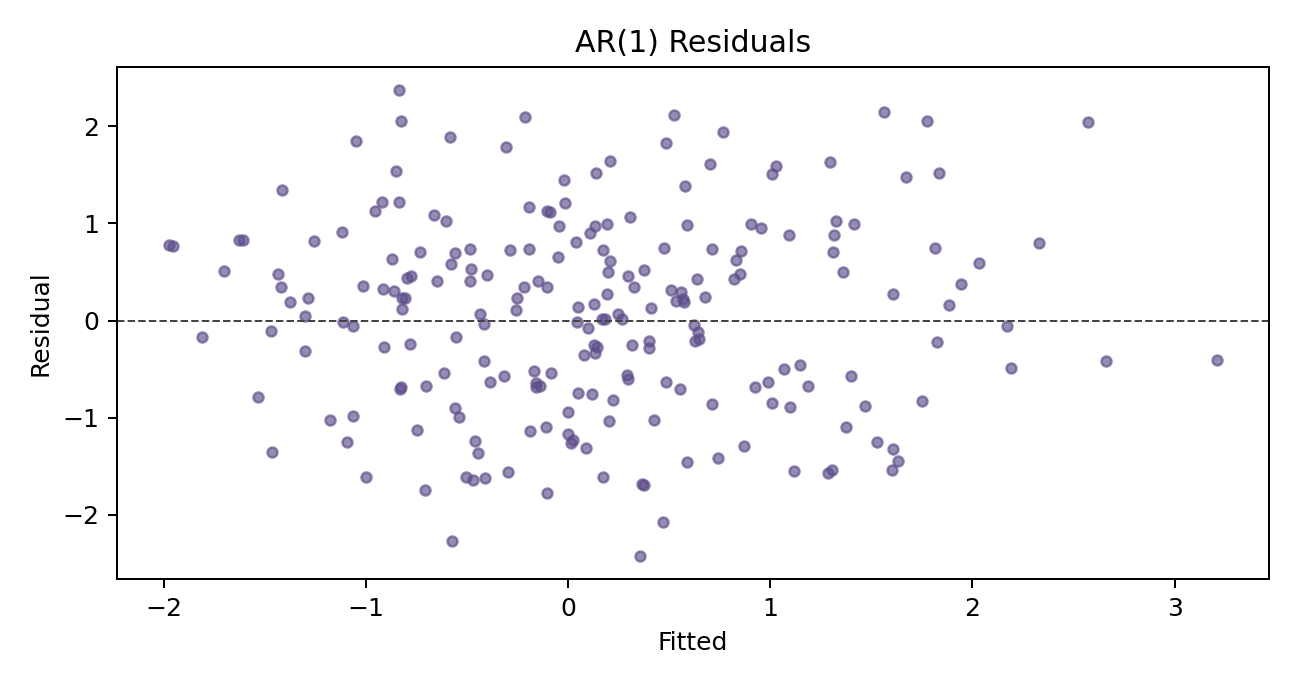
\includegraphics[width=0.86\textwidth]{ch15_fig02_residuals.png}
  \caption{AR(1) 拟合残差图：残差应接近独立同分布创新。}
\end{figure}

\section{练习提要}

原文练习主要围绕下列方向展开：
\begin{itemize}
  \item 手写 AR(1) residual bootstrap 算法；
  \item 比较正态近似区间和 bootstrap 分位数区间；
  \item 研究残差未中心化对 bootstrap 的影响；
  \item 改变 AR 阶数，观察 bootstrap 分布的稳定性。
\end{itemize}

\section*{本章小结}

第 15 章把 bootstrap 引入自回归估计。核心思想是用拟合残差近似未知创新分布，再在拟合模型下重造样本。理论部分说明这种重抽样分布何时能逼近真实估计误差分布。

\clearpage
\appendix
\clearpage
% Source: chapters/appA_background/附录A_Background_背景知识.tex
\chapter{Background / 背景知识}
\section*{本章学习目标}

本章按照原文 \textit{Background} 的小节顺序整理，保留主要定义、定理、模型公式和练习方向，并将原文中的 R 实践思路改写为 Python 工程实践。

完成本章后，应能够：
\begin{itemize}
  \item 复习常用不等式和概率收敛工具；
  \item 理解鞅差和 Burkholder 不等式；
  \item 掌握 Fourier 级数和正交展开；
  \item 理解 FFT 的分治思想；
  \item 为正文中的渐近证明和频域计算提供背景。
\end{itemize}

\section{定义与不等式}

附录首先整理概率界和矩不等式。常用工具包括 Markov 不等式、Chebyshev 不等式、Cauchy-Schwarz 不等式和 Jensen 不等式。例如
\[
  P(|X|>\epsilon)\le \frac{E|X|^p}{\epsilon^p}.
\]

\begin{lemma}[原文 Lemma A.1.1]
若随机变量或随机过程满足给定矩界，则可用最大不等式控制其上确界或部分和，从而推出收敛率。
\end{lemma}

\begin{theorem}[Helly 定理，原文 Theorem A.1.1]
分布函数序列若紧，则存在弱收敛子序列。该结果用于分布收敛的紧性论证。
\end{theorem}

\section{鞅}

\begin{definition}[鞅差，原文 Definition A.2.1]
若 \(E(X_t\mid\mathcal F_{t-1})=0\)，则 \(\{X_t\}\) 关于过滤 \(\{\mathcal F_t\}\) 为鞅差序列。
\end{definition}

鞅差是时间序列渐近理论中的核心对象。许多估计方程可分解为鞅差和小余项，然后用鞅中心极限定理或最大不等式处理。

\section{Fourier 级数}

周期函数可展开为
\[
  f(x)=a_0+\sum_{k=1}^{\infty}\{a_k\cos(kx)+b_k\sin(kx)\}.
\]
复指数形式为
\[
  f(x)=\sum_{k=-\infty}^{\infty}c_ke^{ikx},
  \qquad
  c_k=\frac1{2\pi}\int_{-\pi}^{\pi}f(x)e^{-ikx}\,dx.
\]
正文中的谱密度、DFT 和周期检测都建立在这一正交展开思想上。

\section{Burkholder 不等式与 FFT}

\begin{theorem}[Burkholder 不等式，原文 Theorem A.4.1--A.4.2]
对鞅差部分和 \(S_n=\sum_{t=1}^nY_t\)，其 \(p\) 阶矩可由条件方差和单项矩控制。该工具用于证明时间序列估计中的最大界和收敛率。
\end{theorem}

\section{快速 Fourier 变换}

DFT 定义为
\[
  d(\omega_j)=\sum_{t=0}^{n-1}x_t e^{-i2\pi jt/n}.
\]
当 \(n=2m\) 时，可把偶数项和奇数项分开：
\[
  d_n(j)=d_m^{(even)}(j)+e^{-i2\pi j/n}d_m^{(odd)}(j),
\]
从而递归计算，把复杂度从 \(O(n^2)\) 降到 \(O(n\log n)\)。

\section{Python 工程实践}

在本章目录下运行：
\begin{lstlisting}[language=bash]
python scripts/appA_generate_figures.py
\end{lstlisting}

脚本会把图像写入本章 \texttt{figures/} 目录。当前图像用于配合本章核心概念的仿真说明；若后续补齐原始数据文件，可把模拟数据替换为原文真实数据案例。

\begin{figure}[htbp]
  \centering
  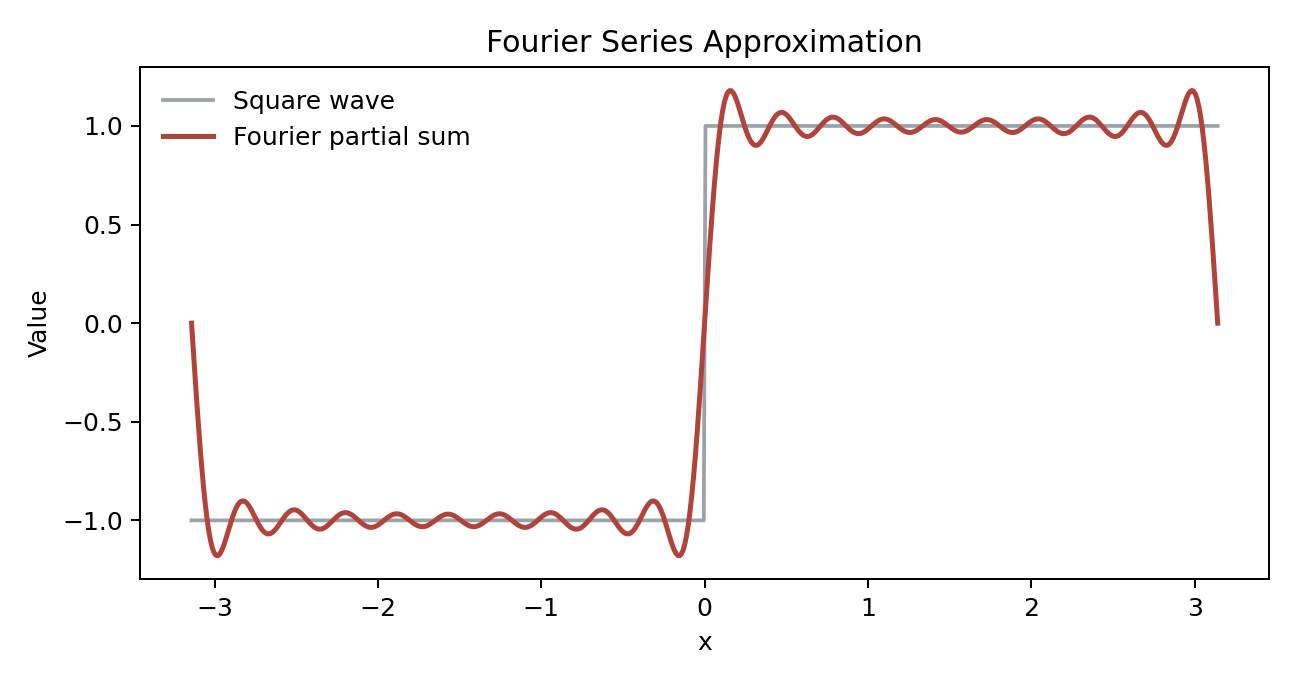
\includegraphics[width=0.86\textwidth]{appA_fig01_fourier_series.png}
  \caption{Fourier 级数近似：用有限个正弦项逼近方波。}
\end{figure}

\begin{figure}[htbp]
  \centering
  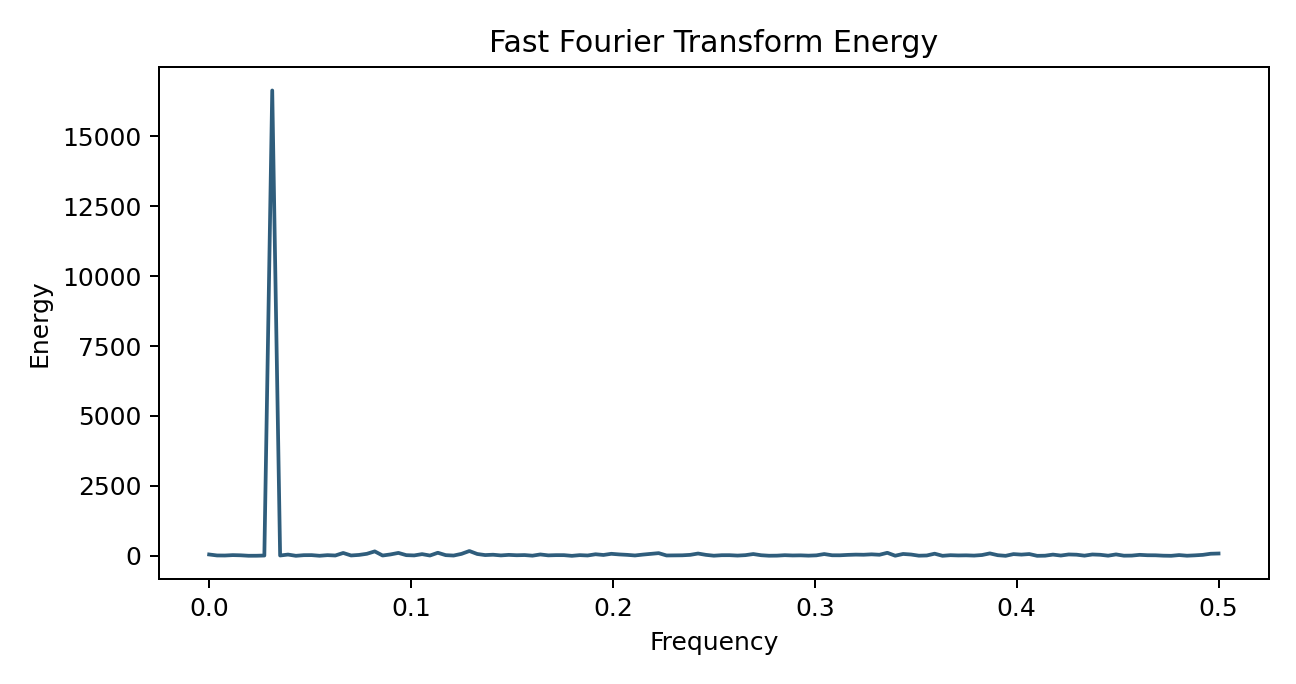
\includegraphics[width=0.86\textwidth]{appA_fig02_fft_energy.png}
  \caption{FFT 能量示例：快速 Fourier 变换用于高效计算频域能量。}
\end{figure}

\section{练习提要}

原文练习主要围绕下列方向展开：
\begin{itemize}
  \item 用 Markov 和 Chebyshev 不等式证明简单概率界；
  \item 验证鞅差的条件期望为 0；
  \item 计算简单周期函数的 Fourier 系数；
  \item 手推 \(n=4\) 时 FFT 的偶奇分解。
\end{itemize}

\section*{本章小结}

附录 A 收集正文所需的概率和分析工具。鞅不等式支撑渐近证明，Fourier 级数和 FFT 支撑频域表示与计算。

\clearpage
% Source: chapters/appB_mixingales_and_physical_dependence/附录B_Mixingales_physical_dependence_Mixingales与物理依赖.tex
\chapter{Mixingales and physical dependence / Mixingales 与物理依赖}
\section*{本章学习目标}

本章按照原文 \textit{Mixingales and physical dependence} 的小节顺序整理，保留主要定义、定理、模型公式和练习方向，并将原文中的 R 实践思路改写为 Python 工程实践。

完成本章后，应能够：
\begin{itemize}
  \item 定义 mixingale 并理解其依赖衰减含义；
  \item 获得几乎必然收敛率；
  \item 理解 Theorem 14.7.3 的证明结构；
  \item 掌握物理依赖度量；
  \item 把 ARMA 过程放入依赖衰减框架。
\end{itemize}

\section{Mixingale}

\begin{definition}[Mixingale，原文 Definition B.0.1]
设 \(\mathcal F_t\) 为过滤。若随机变量 \(X_t\) 满足对过去和未来条件期望的影响随滞后衰减，例如
\[
  \|E(X_t\mid\mathcal F_{t-m})\|_p\le c_t\psi_m,
\]
其中 \(\psi_m\to0\)，则称 \(\{X_t\}\) 为 mixingale。
\end{definition}

\begin{lemma}[分解，原文 Lemma B.0.1]
mixingale 可分解成若干近似鞅差项和可控余项，因此能使用鞅工具证明收敛。
\end{lemma}

\section{几乎必然收敛率}

\begin{lemma}[原文 Lemma B.1.1]
若随机序列 \(S_T\) 的最大二阶矩满足
\[
  E\left(\sup_{t\le T}|S_t|^2\right)\le \phi(T),
\]
则可通过分块和 Borel-Cantelli 引理得到几乎必然收敛率。
\end{lemma}

该节服务于第 14 章估计量收敛率证明：不仅要知道误差趋于 0，还要知道趋于 0 的速度。

\section{Theorem 14.7.3 的证明}

原文证明 ARMA 过程在根离单位圆条件下具有足够快的依赖衰减。若
\[
  X_t=\sum_{j=0}^{\infty}\psi_j\varepsilon_{t-j},
\]
且 \(|\psi_j|\) 几何衰减，则远过去创新对当前的影响迅速变小。

\begin{lemma}[ARMA mixingale 性质，原文 Lemma B.2.1--B.2.2]
满足因果可逆条件的 ARMA 过程可构造为 mixingale，并满足第 14 章所需的几乎必然界。
\end{lemma}

\section{物理依赖性质}

物理依赖度量把过程写成
\[
  X_t=G(\ldots,\varepsilon_{t-1},\varepsilon_t).
\]
将某个过去创新 \(\varepsilon_{t-k}\) 替换为独立副本，得到耦合变量 \(X_t^{*(t-k)}\)。依赖度量定义为
\[
  \delta_p(k)=\|X_t-X_t^{*(t-k)}\|_p.
\]
若 \(\delta_p(k)\) 快速衰减，说明遥远冲击对当前影响很小。

\begin{lemma}[原文 Lemma B.3.1]
在适当 \(p\) 阶矩和物理依赖可和条件下，可得到部分和、样本协方差和估计量所需的矩界。
\end{lemma}

\section{Python 工程实践}

在本章目录下运行：
\begin{lstlisting}[language=bash]
python scripts/appB_generate_figures.py
\end{lstlisting}

脚本会把图像写入本章 \texttt{figures/} 目录。当前图像用于配合本章核心概念的仿真说明；若后续补齐原始数据文件，可把模拟数据替换为原文真实数据案例。

\begin{figure}[htbp]
  \centering
  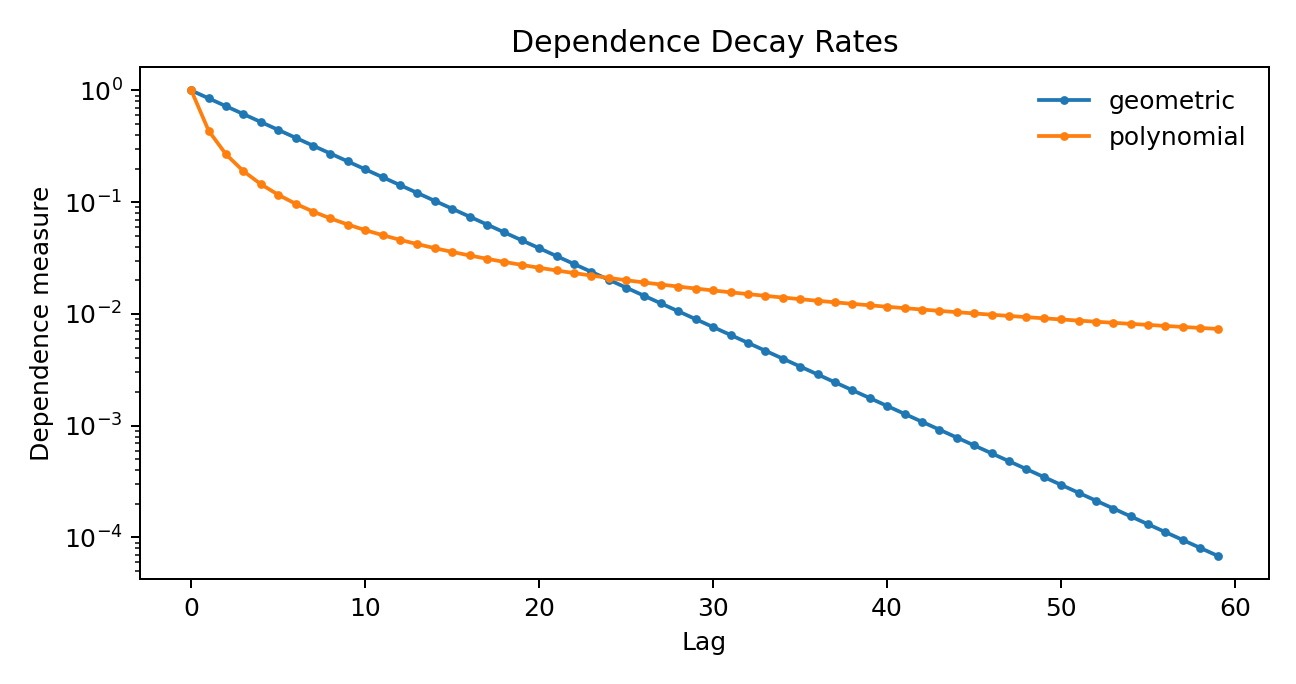
\includegraphics[width=0.86\textwidth]{appB_fig01_dependence_decay.png}
  \caption{依赖衰减率：几何衰减通常比多项式衰减带来更强的渐近结果。}
\end{figure}

\begin{figure}[htbp]
  \centering
  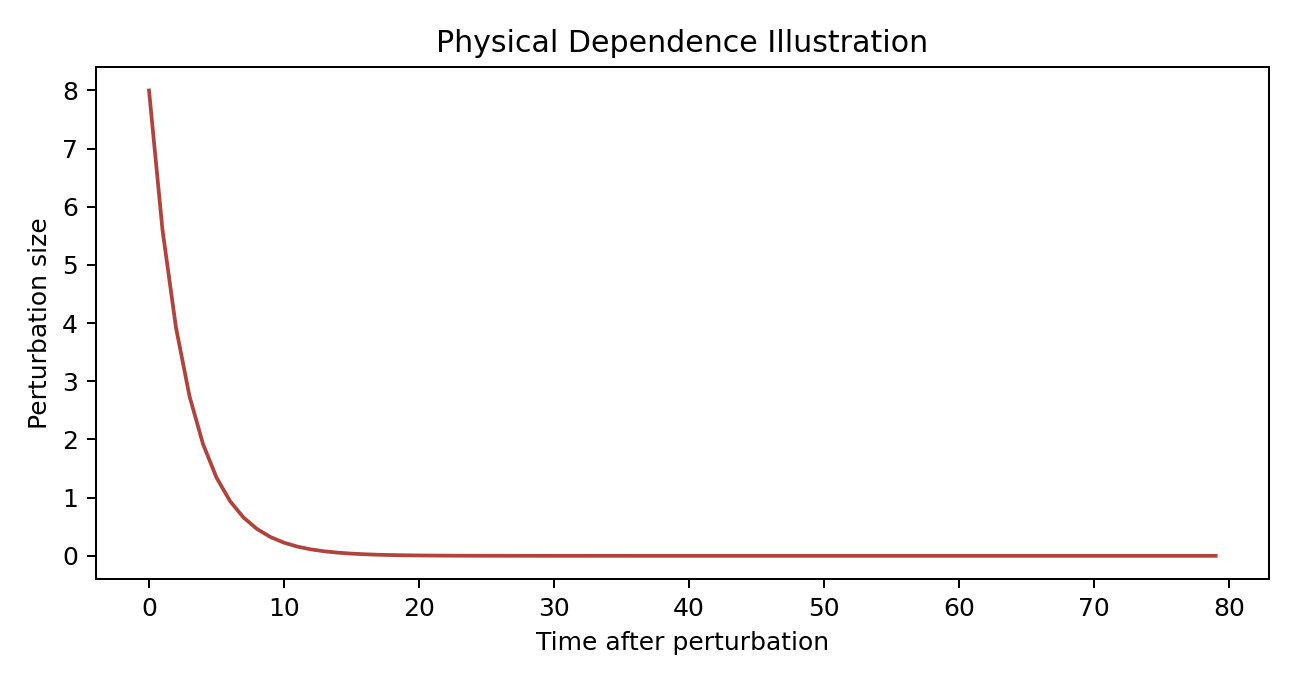
\includegraphics[width=0.86\textwidth]{appB_fig02_physical_dependence.png}
  \caption{物理依赖示意：替换一个早期冲击后，其影响随时间逐渐消失。}
\end{figure}

\section{练习提要}

原文练习主要围绕下列方向展开：
\begin{itemize}
  \item 验证简单 MA(q) 过程的 mixingale 条件；
  \item 用分块法推出几乎必然收敛率；
  \item 计算 AR(1) 的物理依赖度量；
  \item 比较几何衰减和多项式衰减对定理条件的影响。
\end{itemize}

\section*{本章小结}

附录 B 提供处理弱依赖过程的技术框架。Mixingale 和物理依赖都在量化“远处冲击影响变小”，它们是第 14 章渐近证明背后的依赖控制工具。


\end{document}
